\chapter{Gelijkstroomtheorie}
\label{cha:gelijkstroomtheorie}

\newif\ifeen
\newif\ifgestuurdebronnen
\newif\ifknooppunt
\newif\ifmaasstroom
\newif\ifopgaven

\eentrue
\gestuurdebronnentrue
\knooppunttrue
\maasstroomtrue
\opgaventrue


\ifeen

In dit hoofdstuk behandelen we de gelijkstroomtheorie. Nu suggereert het woord
gelijkstroomtheorie dat de theorie alleen de stromen betreft. Dat is echter niet
het geval; het betreft ook de spanningen. We kunnen dus net zo goed spreken over
gelijkspanningstheorie. De keuze voor gelijkstroomtheorie is ingegeven doordat de
grootheid elektrische stroom als een van de zeven grondgrootheden in
het SI-stelsel is gekozen.

In de gelijkstroomtheorie veronderstellen we dat de alle spanningen en stromen
een constante waarden hebben over de tijd. De spanningen en stromen variëren
dus niet als functie van de tijd\footnote{Formeel gezien is een spanning of stroom
die niet van polariteit veranderd ook een gelijkspanning of gelijkstroom. We
veronderstellen hier echter dat de spanningen en stromen constant zijn.}.
Ze kunnen zowel positief als negatief zijn, of nul.

We beginnen dit hoofdstuk met enkele eenvoudige wetten en regels zoals de spannings-
en stroomwetten van Kirchhoff, de wet van Ohm, serie- en parallelschakeling van
weerstanden, spanningsdeling en stroomdeling.
De theorema's van Thévenin en Norton laten zien dat spanningsbronnen en stroombronnen
uitgewisseld kunnen worden. Deze theorema's zijn handig bij het bepalen van
maximale vermogensoverdracht. Het superpositiebeginsel is een eenvoudige methode
om de stromen en spanningen in een netwerk te bepalen en werkt goed met de
eerder genoemde eenvoudige methoden.
Het is echter niet altijd mogelijk de spanningen en stromen in een netwerk met
deze eenvoudige methoden te bepalen. We laten twee methoden zien, de
knooppuntspanningsmethode en maasstroommethode, die bruikbaar zijn in elk netwerk,
hoe complex ze ook zijn. Hierbij moet worden opgemerkt dat kennis van matrixrekenkunde
nodig is. De knooppuntspanningsmethode wordt ook gebruikt in netwerksimulatieprogramma's.

In de gelijkstroomtheorie hebben we drie componenten: de ideale spanningsbron,
de ideale stroombron en de ideale weerstand. De symbolen die gebruikt worden in
schakelschema's zijn te zien in figuur~\ref{fig:gelsymbolenbronnenenweerstand}. Een
ideale spanningsbron levert een constante spanning ongeacht de stroom die de bron
levert. Een ideale stroombron levert een constante stroom ongeacht de spanning die
over de bron staat. Een ideale weerstand heeft een constante waarde ongeacht de
spanning over en de stroom door de weerstand. Verder merken we op dat de ideale
spanningsbron een interne weerstand heeft van 0 Ohm. De interne weerstand van de
ideale stroombron is oneindig.

\begin{figure}[!ht]
\centering
\begin{subfigure}[t]{0.30\textwidth}
\centering
\begin{tikzpicture}[line width=1pt]
\draw (0,0) to [V=$U$] (0,2);
\end{tikzpicture}
\caption{Symbool ideale spanningsbron.}
%\label{fig:gelidealespanningsbron}
\end{subfigure}
\begin{subfigure}[t]{0.30\textwidth}
\centering
\begin{tikzpicture}[line width=1pt]
\draw (0,0) to [I, l=$I$] (0,2);
%\node[left=2pt] at (I.n) {$I$};
\end{tikzpicture}
\caption{Symbool ideale stroombron.}
\end{subfigure}
\begin{subfigure}[t]{0.30\textwidth}
\centering
\begin{tikzpicture}[line width=1pt]
\draw (0,0) to [R, l=$R$] (0,2);
\end{tikzpicture}
\caption{Symbool ideale\\ weerstand.}
\end{subfigure}
%\caption{blabla \protect\subref{fig:gelidealespanningsbron} blabla}
\caption{Symbolen voor de ideale spanningsbron, de ideale stroombron en de ideale weerstand.}
\label{fig:gelsymbolenbronnenenweerstand}
\end{figure}

In de boven gegeven beschrijvingen noemen we de ideale spanningsbron en ideale stroombron
\textsl{onafhankelijke bronnen}. Dat wil zeggen dat de spanning of stroom die de bron
levert niet afhankelijk is van een andere spanning of stroom in een netwerk.
%We zullen verderop kennis maken met afhankelijke bronnen.

Naast de eerder genoemde componenten zijn er nog vier zogenoemde \textsl{gestuurde bronnen}.
De symbolen van deze netwerkelementen zijn te zien in figuur~\ref{fig:gelsymbolengestuuurdebronnenen}.
De spanningsgestuurde spanningsbron levert een constante spanning die afhankelijk is van een
andere spanning in het netwerk. De verhouding tussen de geleverde spanning en de andere spanning
in het netwerk is constant. Hierdoor is de spanningsgestuurde spanningsbron een lineair netwerkelement.
Een stroomgestuurde spanningsbron levert een constante spanning die afhankelijk is van een stroom in
het netwerk. Ook deze verhouding is constant en is de stroomgestuurde spanningsbron een lineair
netwerkelement. Verder zijn er nog de spanningsgestuurde stroombron en de stroomgestuurde stroombron.

\begin{figure}[!ht]
\centering
\begin{subfigure}[t]{0.23\textwidth}
\centering
\begin{tikzpicture}[line width=1pt]
\draw (0,0) to[cV, v=$aU$] ++(0,2);
\end{tikzpicture}
\caption{Symbool spanningsgestuurde spanningsbron.}
%\label{fig:gelidealespanningsbron}
\end{subfigure}
\begin{subfigure}[t]{0.23\textwidth}
\centering
\begin{tikzpicture}[line width=1pt]
\draw (2,0) to[cV, v=$bI$] ++(0,2);
%\node[left=2pt] at (I.n) {$I$};
\end{tikzpicture}
\caption{Symbool stroomgestuurde spanningsbron.}
\end{subfigure}
\begin{subfigure}[t]{0.23\textwidth}
\centering
\begin{tikzpicture}[line width=1pt]
\draw (4,0) to[cI, i_>=,l=$cU\,$] ++(0,2);
\end{tikzpicture}
\caption{Symbool spanningsgestuurde stroombron.}
\end{subfigure}
\begin{subfigure}[t]{0.23\textwidth}
\centering
\begin{tikzpicture}[line width=1pt]
\draw (6,0) to[cI, l=$dI\ $] ++(0,2);
\end{tikzpicture}
\caption{Symbool stroomgestuurde stroombron.}
\end{subfigure}
%\caption{blabla \protect\subref{fig:gelidealespanningsbron} blabla}
\caption{Symbolen voor gestuurde bronnen.}
\label{fig:gelsymbolengestuuurdebronnenen}
\end{figure}

Voor het aangeven van spanningen gebruiken we de hoofdletter $U$. In Engelstalige boeken
wordt de hoofdletter $V$ gebruikt. Spanning worden uitgedrukt in \si{\volt} (volt). Stromen
worden aangegeven met een hoofdletter $I$ en worden uitgedrukt in \si{\ampere} (amp\`ere).
Weerstanden geven we aan met de hoofdletter $R$ (van het Engelse woord \textsl{resistor})
en worden uitgedrukt in \si{\ohm} (ohm).

We kunnen de waarden van spanningen, stromen en weerstanden ook uitdrukken door er een
letter voor te zetten, de zogenoemde SI-voorvoegsels: \si{\milli\volt} (millivolt),
\si{\milli\ampere} (milliamp\`ere), \si{\micro\ampere} (microamp\`ere), \si{\kilo\ohm}
(kilo-ohm), \si{\mega\ohm} (megaohm).

\subsubsection*{Nulstelling}
Met nulstelling bedoelen we het op nul stellen van een bepaalde bron. Een spanningsbron
van \SI{0}{\volt} mag vervangen worden door een kortsluiting. Een stroombron met de
waarde~\SI{0}{\ampere} mag uit het netwerk verwijderd worden. De nulstelling van bronnen
wordt gebruikt bij het superpositiebeginsel (zie paragraaf~\ref{sec:gelsuperpositie}).

\subsubsection*{Fundamentele wetten}
Alle berekeningen in een gelijkstroomnetwerk zijn terug te brengen tot drie wetten:
\begin{itemize}
\item De stroomwet van Kirchhoff;
\item De spanningswet van Kirchhoff;
\item De wet van Ohm.
\end{itemize}
We zullen deze wetten eerst bespreken voordat we andere wetten en berekeningsmethoden bespreken.

\section{De stroomwet van Kirchhoff}
De stroomwet van Kirchhoff zegt dat alle stromen naar een knooppunt toe opgeteld 0 zijn.
Er kan dus geen stroom bijkomen of verloren gaan. In formulevorm:
\begin{equation}
I_1 + I_2 + \cdots + I_n = 0
\end{equation}
Ander gezegd: de totale stroom die naar een knooppunt toevloeit is even groot als de
totale stroom die van het knooppunt wegvloeit. In figuur~\ref{fig:gelstroomwetKirchhoff}
is de stroomwet uitgebeeld.

\begin{figure}[!ht]
\centering
\begin{tikzpicture}[line width=1pt]
\draw (-2,1) to [short, i=$I_1$, -*] (0,0);
\draw (-1.5,-1.5) to [short, i=$I_2$, -*] (0,0);
\draw (2,0.5) to [short, i=$I_3$, -*] (0,0);
\draw (1,-1.5) to [short, i=$I_4$, -*] (0,0);
\end{tikzpicture}
\caption{De stroomwet van Kirchhoff: de stromen naar een knooppunt toe zijn opgeteld 0.}
\label{fig:gelstroomwetKirchhoff}
\end{figure}

In het geval dat een knooppunt slechts twee aansluitingen heeft, is de ingaande stroom even groot als de
uitgaande stroom. Zie figuur~\ref{fig:gelingaandeIisuitgaandeI}.

\begin{figure}[!ht]
\centering
\begin{tikzpicture}[line width=1pt]
\draw (0,0) to [short, i>=$I_1$, -*] ++(3,0) node[above,yshift=.6cm] {$I_1=I_2$} to [short, i>=$I_2$] ++(3,0);
\end{tikzpicture}
\caption{De ingaande stroom is even groot als de uitgaande stroom.}
\label{fig:gelingaandeIisuitgaandeI}
\end{figure}

\begin{example}[De stroomwet van Kirchhoff]
In figuur~\ref{fig:gelstroomwetKirchhoff2} is een netwerk getekend van vier stroomvoerende geleiders.
Bepaal de stroom $I$.
\begin{center}
\centering
\begin{tikzpicture}[line width=1pt]
\draw (-2,1) to [short, i=\SI{5}{\ampere}, -*] (0,0);
\draw (-1.5,-1.5) to [short, i<=\SI{2}{\ampere}, -*] (0,0);
\draw (2,0.5) to [short, i=\SI{3}{\ampere}, -*] (0,0);
\draw (1,-1.5) to [short, i=$I$, -*] (0,0);
\end{tikzpicture}
\captionof{figure}{De stroomwet van Kirchhoff.}
\label{fig:gelstroomwetKirchhoff2}
\end{center}
Oplossing: Volgens de stroomwet van Kirchhoff moeten alle stromen opgeteld naar een knooppunt 0 zijn.
Let hierbij op de referentierichtingen van de stromen. Zo is de referentierichting van de stroom van
\SI{2}{\ampere} van het knooppunt af getekend. We kunnen dus stellen dat:
\begin{equation}
\SI{5}{\ampere} - \SI{2}{\ampere} + \SI{3}{\ampere} + I = 0
\end{equation}
De betekent dat $I = \SI{-6}{\ampere}$ is. Let hierbij op het minteken.
\end{example}


\section{De spanningswet van Kirchhoff}
De spanningswet van Kirchhoff zegt dat alle spanningen in een gesloten kring opgeteld~0
zijn. Er kan dus geen spanning bijkomen of verloren gaan. In formulevorm:
%
\begin{equation}
U_1 + U_2 + \cdots + U_n = 0
\end{equation}

Anders gezegd: de totale spanning rechtsom opgeteld, is even groot als de totale spanning linksom opgeteld. In figuur~\ref{fig:spanningswetKirchhoff} is de spanningswet uitgebeeld.

\begin{figure}[!ht]
\centering
\begin{tikzpicture}[line width=1pt]
\draw (0.0,0.0)  node[left] {$+$} to [short, o-] ++(0.0,1.0) to [short, -o]  node[above] {$-$} ++(1.0,0.0)
      to [open,l=$U_2$,above] ++(0.5,0.0) node[above] {$+$} to [short, o-] ++(1.0,0.0) to [short, -o] node[right] {$-$} ++(0.0,-1.0)
      to [open,l=$U_3$,above] ++(0.0,-0.5) node[right] {$+$} to [short, o-] ++(0.0,-1.0) to [short, -o] node[below] {$-$} ++(-1.0,0.0)
      to [open,l=$U_4$,above] ++(-0.5,0.0) node[below] {$+$} to [short, o-] ++(-1.0,0.0) to [short, -o] node[left] {$-$} ++(0.0,1.0)
      to [open,l=$U_1$,above] ++(0.0,0.5);
\end{tikzpicture}
\caption{De spanningswet van Kirchhoff: alle spanningen in een kring zijn opgeteld 0.}
\label{fig:spanningswetKirchhoff}
\end{figure}

Als een verbinding zich vertakt over twee parallel geschakelde netwerkelementen dan is de spanning over
de netwerkelementen gelijk. Dit is te zien in figuur~\ref{fig:gelspanningengelijk}.

\begin{figure}[!ht]
\centering
\begin{tikzpicture}[line width=1pt]
\draw (0,0) to[short,-*]++(1,0) to[short] ++(0,0.5) to[short,-o,] node[above] {$+$} ++(1,0) to[open, l=$U_1$,above] ++(1,0) node[above] {$-$} to[short, o-] ++(1,0) to[short,-*] ++(0,-.5) to[short] ++(1,0) to[open] ++(-1,0) to[short] ++(0,-0.5) to[short,-o] node[below] {$-$} ++(-1,0) to [open,l=$U_2$,-o] ++(-1,0) node[below] {$+$} to [short] ++(-1,0) to [short] ++(0,0.5);
\draw (0,1) node {$U_1=U_2$};
\end{tikzpicture}
\caption{De spanningen over twee parallel geschakelde elementen zijn gelijk.}
\label{fig:gelspanningengelijk}
\end{figure}

\begin{example}[De spanningswet van Kirchhoff]
In figuur~\ref{fig:gelspanningswetKirchhoff2} is een netwerk getekend van vier spanningsbronnen.
Bepaal de spanning~$U$.
\begin{center}
\centering
\begin{tikzpicture}[line width=1pt]
\draw (0,0) to[V, v=\SI{5}{\volt}] (0,2)
            to[V, v<=\SI{-2}{\volt}] (2,2)
            to[V, v<=$U$] (2,0)
			to[V, v=\SI{3}{\volt}] (0,0);
\end{tikzpicture}
\captionof{figure}{De spanningswet van Kirchhoff.}
\label{fig:gelspanningswetKirchhoff2}
\end{center}
Oplossing: Volgens de spanningswet van Kirchhoff moeten alle spanningen in kring opgeteld gelijk aan 0 zijn.
Let hierbij op de referentierichtingen en de waarden van de spanningen. Zo is de referentierichting van
de spanningsbron van \SI{-2}{\volt} tegengesteld aan de referentierichting van de spanningsbron van
\SI{5}{\volt}. We kunnen dus stellen dat:
\begin{equation}
\SI{5}{\volt} - (\SI{-2}{\volt}) - U + \SI{3}{\volt} = 0
\end{equation}
De betekent dat $U = \SI{10}{\volt}$ is. Let hierbij op de richting van de spanning $U$.
\end{example}


\section{De wet van Ohm}
De verhouding tussen de spanning over een weerstand en de stroom door de weerstand is constant
en wordt de wet van Ohm genoemd. De wet wordt meestal geschreven als:
\begin{equation}
U=I\cdot R
\end{equation}
%
Gegeven een bepaalde spanning en stroom, dan kan de weerstandswaarde berekend worden met:
%
\begin{equation}
R = \dfrac{U}{I}
\end{equation}
%
In figuur~\ref{fig:geldewetvanohm} is de wet van Ohm uitgebeeld. Aan de spanningsbron $U$ wordt
een weerstand $R$ geplaatst. We spreken dan dat de spanningsbron wordt belast. Ook hier geldt de
spanningswet van Kirchhoff: de spanning $U$ van de bron is gelijk aan de spanning $U_R$ over de
weerstand. Bij de gegeven richting van de stroom $I$ geldt dat het potentiaal bij de `$+$' groter
is dan het potentiaal bij de `$-$'. Over de weerstand treedt \textsl{spanningsval} op.

\begin{figure}[!ht]
\centering
\begin{tikzpicture}[bookcircuit]
\draw (0,0) to [V=$U$] ++(0,2) to [short, i=$I$] ++(2.5,0) to [R=$R$, v=$U_R$] ++(0,-2) to [short,-.] (0,0)
;
%%%\draw (-2,0) to[short, i=$I$] (0,0);
%%%\draw (0,0) to[R=$R$, v_>=$U$] (2,0);
\end{tikzpicture}
\caption{De spanning over en stroom door een weerstand is constant.}
\label{fig:geldewetvanohm}
\end{figure}

\begin{example}[De wet van Ohm]
In figuur~\ref{fig:geldewetvanohm} is de spanning $U=\SI{12}{\volt}$ en de stroom $I=\SI{2}{\milli\ampere}$.
Bereken de waarde van van weerstand $R$.

Oplossing: We gebruiken de wet van Ohm voor het berekenen van de weerstandswaarde. Let erop dat de stroom in milliampère is gegeven:
\begin{equation}
R = \dfrac{12}{\num{2d-3}} = \SI{6000}{\ohm} 
\end{equation}

De waarde van weerstand $R$ is \SI{6000}{\ohm}, oftwel \SI{6}{\kilo\ohm} (kilo-ohm).
\end{example}

\subsection{Geleiding}
\label{sec:gelgeleiding}
In veel berekeningen wordt gerekend met de reciproke (of omgekeerde) waarde van weerstanden. Dit wordt
de \textsl{geleiding} of \textsl{geleidbaarheid} genoemd. De eenheid van geleiding is siemens (\si{\siemens}).
Meestal gebruiken we voor geleiding de letter $G$:
\begin{equation}
\label{equ:geleiding}
G = \dfrac{1}{R}
\end{equation}
In de literatuur wordt ook wel de naam mho (omgekeerde van ohm) gebruikt en als symbool wordt ook wel \si{\mho} of \si{\per\ohm} gebruikt.


\section{Spoel en condensator}
De spoel en de condensator hebben geen actieve rol in een gelijkstroomnetwerk. We bekijken de stroom-spanningrelaties:
%
\begin{equation}
\text{spoel: } u(t) = L\dfrac{\mathrm{d}i(t)}{\mathrm{d}t} \qquad\qquad \text{condensator: } i(t) = C\dfrac{\mathrm{d}u(t)}{\mathrm{d}t}
\end{equation}
%
De spanning over de spoel is recht evenredig met de \textsl{stroomverandering} door de spoel. Er is echter geen verandering van de stroom, de stroom is constant. De spanning over de spoel is dus \SI{0}{\volt}. De spoel gedraagt zich als een kortsluiting.

De stroom door een condensator is recht evenredig met de \textsl{spanningsverandering} over de condensator. De spanning verandert echter niet, de spanning is constant. De stroom door de condensator is dus \SI{0}{\ampere}. Hierdoor gedraagt de condensator zich als twee open klemmen (dit wordt ook wel een open verbinding genoemd).


\section{Serieschakeling van weerstanden}
In figuur~\ref{fig:gelserieschakelingweerstanden} is een schakeling te zien waarbij de weerstanden
in serie geschakeld zijn en gevoed worden door een spanningsbron. De spanningsbron levert een stroom
$I$ waardoor de spanningsbron een bepaalde weerstand ondervindt. We noemen deze weerstand $R_s$.

\begin{figure}[!ht]
\centering
\begin{tikzpicture}[bookcircuit]
\draw (0,0) to [V=$U$] ++ (0,2) to [short, i=$I$] ++(2,0)
            to [R, l=$R_1$,v=$U_1$] ++(2,0) to [R, l=$R_2$, v=$U_2$] ++(2,0)
            coordinate (A);
\draw[dotted] (A) --  ++(1,0) coordinate (B);
\draw (B) to [R,l=$R_n$,v=$U_n$] ++(2,0) to [short] ++(0.5,0) to [short] ++(0,-2) to [short,-.] (0,0);
\end{tikzpicture}
\caption{Serieschakeling van weerstanden.}
\label{fig:gelserieschakelingweerstanden}
\end{figure}

Vanuit de spanningswet van Kirchhoff volgt dat:
%
\begin{equation}
U=U_1+U_2+\cdots+U_n
\end{equation}
%
Vanuit de stroomwet van Kirchhoff volgt dat:
%
\begin{equation}
I = I_1 = I_2 = \cdots = I_n
\end{equation}
%
De stroom die de bron levert is dus even groot als de stromen door de weerstanden.
De bron met spanning $U$ levert een stroom $I$ zodanig dat:
%
\begin{equation}
U=I\cdot R_s
\end{equation}
%
Dus volgt dat:
%
\begin{equation}
I\cdot R_s = I\cdot R_1+I\cdot R_2+\cdots+I\cdot R_n
\end{equation}
%
We schappen aan beide kanten $I$ zodat volgt dat:
%
\begin{equation}
R_s = R_1 + R_2 + \cdots R_n
\end{equation}
%
Hierbij is $R_s$ de vervangingswaarde van de in serie geschakelde weerstanden.

\begin{example}[Berekenen van de serieweerstand]
Gegeven is een serieschakeling van vijf weerstanden met de waarden $R_1=\SI{2.2}{\kilo\ohm}$,
$R_2=\SI{3.3}{\kilo\ohm}$, $R_3=\SI{1.5}{\kilo\ohm}$, $R_4=\SI{1.2}{\kilo\ohm}$ en
$R_5=\SI{4.7}{\kilo\ohm}$. Bereken de vervangingswaarde van de serieweerstand $R_s$.

Oplossing: De vervangingswaarde van de serieweerstand $R_s$ is de som van de waarden van $R_1$
t/m $R_5$. Dus is:
\begin{equation}
\begin{split}
R_s &= R_1 + R_2 + R_3 + R_4 + R_5\\
    &= \SI{2.2}{\kilo\ohm} + \SI{3.3}{\kilo\ohm} +
        \SI{1.5}{\kilo\ohm} + \SI{1.2}{\kilo\ohm} + \SI{4.7}{\kilo\ohm} \\
    &= \SI{12.9}{\kilo\ohm} 
\end{split}
\end{equation}
\end{example}

\section{Parallelschakeling van weerstanden}
In figuur~\ref{fig:gelparalledschakelingweerstanden} is een parallelschakeling van een
aantal weerstanden te zien. De schakeling wordt gevoed door de spanningsbron $U$. Als
gevolg van de weerstanden zal de bron een bepaalde stroom leveren. Hierdoor ondervindt
de spanningsbron een bepaalde weerstand. Deze weerstand noemen we $R_p$.

\begin{figure}[!ht]
\centering
\begin{tikzpicture}[bookcircuit]
%% Draw voltage source, wire with current I, resistor R1 and back to minus of voltage source
\draw (0,0) to [V=$U$] ++ (0,2) to [short] ++(0,0.25) to [short,i=$I$,-*] ++(3,0) coordinate (A) to [short] ++(0,-0.25) to[R=$R_1$,-*,i>^=\small $I_1$,v=\small $U_1$] ++(0,-2) to [short,-.] (0,0);
%% Draw resistor R2 and wire to minus of resistor R1
\draw (A) to[short,-*] ++(2,0) coordinate (B) to [short] ++(0,-0.25) to [R=$R_2$,-*,i>^=\small $I_2$, v=\small $U_2$] ++(0,-2) to [short] ++(-2,0);
%% Draw short heading to Rk
\draw (B) to[short] ++(0.75,0) coordinate (C);
%% Draw dotted wire
\draw[dotted] (C) -- ++(1,0) coordinate (D);  
%% Draw Rk
\draw (D) to [short] ++(0.75,0) to [short] ++(0,-0.25) to [R=$R_n$,i>^=\small $I_n$, v=\small $U_n$ ] ++(0,-2) to [short] ++(-0.75,0) coordinate (E);
%% Draw dotted wire
\draw[dotted] (E) -- ++(-1,0) coordinate (F);
%% Draw wire to minus of R2
\draw (F) to [short] ++(-0.75,0);
\end{tikzpicture}
\caption{Parallelschakeling van weerstanden.}
\label{fig:gelparalledschakelingweerstanden}
\end{figure}

Vanuit de spanningswet van Kirchhoff vinden we dat:
%
\begin{equation}
U = U_1 = U_2 = \cdots = U_n
\end{equation}
%
De spanningen over de weerstanden zijn even groot als de bronspanning.
Vanuit de stroomwet van Kirchhoff vinden we dat:
%
\begin{equation}
I = I_1 + I_2 + \cdots + I_n
\end{equation}
%
We kunnen de stroomwet ook formuleren als:
%
\begin{equation}
\dfrac{U}{R_p} = \dfrac{U}{R_1} + \dfrac{U}{R_2} + \cdots + \dfrac{U}{R_n}
\end{equation}
%
We schrappen aan beide zijden van de vergelijking de spanning $U$ zodat we krijgen dat:
%
%De vervangingswaarde voor de parallelschakeling van een aantal weerstanden is te berekenen met:
\begin{equation}
\dfrac{1}{R_p} = \dfrac{1}{R_1} + \dfrac{1}{R_2} + \cdots + \dfrac{1}{R_n}
\end{equation}
%
Hierin is $R_p$ de vervangingswaarde van de parallel geschakelde weerstanden.
Voor twee parallel geschakelde weerstanden geldt dat:
\begin{equation}
\dfrac{1}{R_p} = \dfrac{1}{R_1} + \dfrac{1}{R_2}
\end{equation}
%
Dit kan worden omgewerkt tot:
%
\begin{equation}
\dfrac{1}{R_p} = \dfrac{R_2}{R_1R_2} + \dfrac{R_1}{R_1R_2} = \dfrac{R_1+R_2}{R_1R_2}
\end{equation}
%
Als we $1/R_p$ omkeren, krijgen we:
\begin{equation}
R_p = \dfrac{R_1\cdot R_2}{R_1+R_2}
\end{equation}

\begin{example}[Berekenen van de parallelweerstand]
Gegeven is een parallelschakeling van drie weerstanden $R_1 = \SI{3.3}{\kilo\ohm}$,
$R_2 = \SI{6.8}{\kilo\ohm}$ en $R_3 = \SI{8.2}{\kilo\ohm}$. Bereken de vervangingswaarde
van de parallelweerstand $R_p$.

Oplossing: Voor de parallelweerstand kunnen we schrijven:
\begin{equation}
\begin{split}
\dfrac{1}{R_p} &= \dfrac{1}{R_1} + \dfrac{1}{R_2} + \dfrac{1}{R_3} \\
               &= \dfrac{1}{\SI{3.3d3}{\ohm}} + \dfrac{1}{\SI{6.8d3}{\ohm}} + \dfrac{1}{\SI{8.2d3}{\ohm}} \\[1ex]
               &= \SI{0,572e-3}{\siemens}
\end{split}
\end{equation}
%
Dus geldt voor $R_p$:
\begin{equation}
R_p = \dfrac{1}{\SI{0,572e-3}{\siemens}} = \SI{1,748}{\kilo\ohm}
\end{equation}
\end{example}

\section{Serie- en parallelschakeling van geleidingen}
Met behulp van~\eqref{equ:geleiding} kunnen we de formules afleiden voor serie- en parallelschakeling van geleidingen. Voor serieschakeling van geleidingen geldt:
%
\begin{equation}
\dfrac{1}{G_s} = \dfrac{1}{G_1} + \dfrac{1}{G_2} + \cdots + \dfrac{1}{G_n}
\end{equation}
%
Voor parallelschakeling van geleidingen geldt:
%
\begin{equation}
G_p = G_1 + G_2 + \cdots + G_n
\end{equation}


\section{Spanningsdeling}
In figuur~\ref{fig:gelspanningsdeling} is een netwerk te zien van een bron met twee in
serie geschakelde weerstanden. De spanning $U$ zal zich in een bepaalde verhouding
verdelen over de twee weerstanden. Er is sprake van spanningsdeling.

\begin{figure}[!ht]
\centering
\begin{tikzpicture}[bookcircuit]
\draw (0,0) to [V=$U$] ++ (0,2) to [short, i=$I$] ++(1.5,0)
            to [R, l=$R_1$,v=$U_1$] ++(2,0) to [R, l=$R_2$, v=$U_2$] ++(2,0)
            to [short] ++(0.5,0) to [short] ++(0,-2) to [short,-.] (0,0);
\end{tikzpicture}
\caption{Netwerk voor spanningsdeling.}
\label{fig:gelspanningsdeling}
\end{figure}

De stroom $I$ kunnen we berekenen met:
%
\begin{equation}
I = \dfrac{U}{R_1+R_2}
\end{equation} 
%
Voor de spanningen $U_1$ en $U_2$ kunnen we schrijven dat:
%
\begin{equation}
U_1 = I\cdot R_1 = \dfrac{R_1}{R_1+R_2}\cdot U \qquad\text{en}\qquad U_2 = I\cdot R_2 = \dfrac{R_2}{R_1+R_2}\cdot U
\end{equation}

\begin{example}[Spanningsdeling]
Gegeven is het netwerk in figuur~\ref{fig:gelspanningsdeling}. Hierin zijn $U=\SI{12}{\volt}$, $R_1=\SI{2.2}{\kilo\ohm}$
en $R_2=\SI{3.9}{\kilo\ohm}$. Bereken de spanning $U_2$.

Oplossing: We vullen de gegevens in de formule in:
\begin{equation}
U_2 = I\cdot R_2 = \dfrac{R_2}{R_1+R_2}\cdot U = \dfrac{\SI{3.9}{\kilo\ohm}}{\SI{2.2}{\kilo\ohm}+\SI{3.9}{\kilo\ohm}}\cdot\SI{12}{\volt} = \SI{7.67}{\volt}
\end{equation}
\end{example}


\section{Stroomdeling}
In figuur~\ref{fig:gelstroomdeling} is een netwerk te zien van een bron met twee parallel
geschakelde weerstanden. De stroom $I$ zal zich in een bepaalde verhouding
verdelen over de twee weerstanden. Er is sprake van stroomdeling.

\begin{figure}[!ht]
\centering
\begin{tikzpicture}[bookcircuit]
%% Draw voltage source, wire with current I, resistor R1 and back to minus of voltage source
\draw (0,0) to [I,l=$I$] ++ (0,2) to [short] ++(0,0.25) to [short,i=$I$,-*] ++(3,0) coordinate (A) to [short] ++(0,-0.25) to[R=$R_1$,-*,i>^=\small $I_1$,v=\small $U$] ++(0,-2) to [short,-.] (0,0);
%% Draw resistor R2 and wire to minus of resistor R1
\draw (A) to[short] ++(2,0) coordinate (B) to [short] ++(0,-0.25) to [R=$R_2$,i>^=\small $I_2$, v=\small $U$] ++(0,-2) to [short] ++(-2,0);
\end{tikzpicture}
\caption{Netwerk voor stroomdeling.}
\label{fig:gelstroomdeling}
\end{figure}

De spanning $U$ kunnen we berekenen met:
%
\begin{equation}
U = I\cdot\dfrac{R_1\cdot R_2}{R_1+R_2}
\end{equation}
%
Natuurlijk geldt de stroomwet van Kirchhoff:
%
\begin{equation}
I = I_1 + I_2 = \dfrac{U}{R_1} + \dfrac{U}{R_2}
\end{equation}
%
Voor $I_1$ geldt dan:
%
\begin{equation}
I_1 = \dfrac{U}{R_1} = \dfrac{1}{R_1}\cdot\dfrac{R_1\cdot R_2}{R_1+R_2}\cdot I = \dfrac{R_2}{R_!+R_2}\cdot I
\end{equation}
%
Op vergelijkbare wijze vinden we voor $I_2$:
%
\begin{equation}
I_2 = \dfrac{U}{R_2} = \dfrac{1}{R_2}\cdot\dfrac{R_1\cdot R_2}{R_1+R_2}\cdot I = \dfrac{R_1}{R_!+R_2}\cdot I
\end{equation}

\begin{example}[Stroomdeling]
Gegeven is het netwerk in figuur~\ref{fig:gelstroomdeling2}. Hierin zijn $I=\SI{2}{\ampere}$, $R_1=\SI{6}{\ohm}$,
$R_2=\SI{9}{\ohm}$ en $R_3=\SI{12}{\ohm}$. Bereken de stroom $I_3$.
\begin{figure}[H]
\centering
\begin{tikzpicture}[bookcircuit]
%% Draw voltage source, wire with current I, resistor R1 and back to minus of voltage source
\draw (0,0) to [I,l=$I$] ++ (0,2) to [short,i=$I$,-*] ++(3,0) coordinate (A) to[R=$R_1$,-*,i>^=\small $I_1$] ++(0,-2) to [short,-.] (0,0);
%% Draw resistor R2 and wire to minus of resistor R1
\draw (A) to[short] ++(2,0) coordinate (B) to [R=$R_2$,i>^=\small $I_2$,-*] ++(0,-2) to [short] ++(-2,0);
\draw (B) to[short] ++(2,0) coordinate (C) to [R=$R_3$,i>^=\small $I_3$] ++(0,-2) to [short] ++(-2,0);
\end{tikzpicture}
\caption{Netwerk voor stroomdeling.}
\label{fig:gelstroomdeling2}
\end{figure}
Oplossing: De totale stroom die de bron levert is $I=\SI{2}{\ampere}$. Om gebruik te maken van de formules
voor stroomdeling moeten we het netwerk vereenvoudigen tot een stroombron met twee weerstanden. We vervangen
de weerstanden $R_1$ en $R_2$ door een weerstand $R_p$. De vervangingswaarde is:
\begin{equation}
R_p = \dfrac{R_1R_2}{R_1+R_2} = \dfrac{6\cdot9}{6+9} = \SI{3.6}{\ohm}
\end{equation}
Nu kunnen we de stroom $I_3$ uitrekenen:
\begin{equation}
I_3 = \dfrac{R_p}{R_P+R_3}\cdot I = \dfrac{\num{3.6}}{\num{3.6}+\num{12}}\cdot \num{2} = \SI{0.46}{\ampere}
\end{equation}
\end{example}


\section{De niet-ideale spanningsbron}
\label{sec:gelnietidealespanningsbron}
In de praktijk hebben we te maken met niet-ideale spanningsbronnen. We kunnen zo'n bron
weergeven met een ideale spanningsbron in serie met een ideale weerstand. De ideale
weerstand wordt de \textsl{inwendige weerstand} genoemd. Dit is te zien in
\index{inwendige weerstand}
figuur~\ref{fig:gelnisopenkort}.

\begin{figure}[!ht]
\begin{subfigure}{0.5\textwidth}
\centering
\begin{tikzpicture}[bookcircuit]
\draw (0,0) to [V=$U$] ++(0,2) to [R=$R_i$,-*] coordinate (A) ++(2.5,0) node[right] {$+$} to [open] ++(0,-2) coordinate (B) node[right] {$-$} to [short,*-.] (0,0);
\draw ($(A)!0.5!(B)$) node[right] {$U_o$};
\end{tikzpicture}
\caption{}
\label{fig:gelnisopen}
\end{subfigure}%
\begin{subfigure}{0.5\textwidth}
\centering
\begin{tikzpicture}[bookcircuit]
\draw (0,0) to [V=$U$] ++(0,2) to [R=$R_i$,-*] ++(2.5,0) to [short, i=$I_k$] ++(0,-2) to [short,*-.] (0,0);
\end{tikzpicture}
\caption{}
\label{fig:gelniskort}
\end{subfigure}
\caption{Niet-ideale spanningsbron: \subref{fig:gelnisopen} open, onbelast, \subref{fig:gelniskort} kortgesloten, belast.}
\label{fig:gelnisopenkort}
\end{figure}

In figuur~\ref{fig:gelnisopen} is te zien dat de niet-ideale spanningsbron onbelast is.
De spanning $U_o$ is even groot als de bronspanning $U$. Er loopt immers geen stroom zodat
er geen spanningsval over de inwendige weerstand staat. Deze spanning wordt de \textsl{open
klemspanning} genoemd. In figuur~\ref{fig:gelniskort} is
\index{open klemspanning}
de niet-ideale spanningsbron kortgesloten. Over de inwendige weerstand staat nu de volledige
bronspanning. Er loopt dan een zekere \textsl{kortsluitstroom} $I_k$. We kunnen de inwendige
\index{kortsluitstroom}
weerstand berekenen door de uitgangsspanning $U_o$ te delen door de kortsluitstroom $I_k$.

Voor een goede spanningsbron moet de inwendige weerstand klein zijn. Praktische waarden van
de inwendige weerstanden liggen tussen de enkele tientallen \si{\milli\ohm} tot enkele \si{\ohm}.
Zo kan een autoaccu met een spanning van \SI{12}{\volt} stromen van meer dan \SI{100}{\ampere}
leveren. Het is dan
ook niet aan te bevelen om dergelijke kortsluitstromen te meten. De inwendige weerstand
van eenvoudige batterijen ligt in de orde van enkele \si{\ohm}. Een laboratoriumvoeding moet
natuurlijk ook een lage inwendige weerstand hebben om de uitgangsspanning zo constant
mogelijk te houden. Veelal is de voeding beschermd tegen kortsluiting en wordt de
kortsluitstroom begrensd.


\section{De niet-ideale stroombron}
\label{sec:gelnietidealestroombron}
In de praktijk hebben we ook te maken met niet-ideale stroombronnen. De niet-ideale
stroombron is te modelleren als een ideale stroombron parallel geschakeld aan een ideale
weerstand. Ook deze weerstand wordt de inwendige weerstand genoemd. Dit is te zien in
figuur~\ref{fig:gelnissopenkort}.

\begin{figure}[!ht]
\begin{subfigure}{0.5\textwidth}
\centering
\begin{tikzpicture}[bookcircuit]
\draw (0,0) to [I, l=$I$, inner sep=5pt] ++(0,2) to [short] ++(1,0) coordinate (A) to [R=$R_i$,*-*]  ++(0,-2) coordinate (B) to [short,-.] (0,0) (A) to [short, -*] ++(1,0) node[right] {$+$} (B) to [short, -*] ++(1,0) node[right] {$-$}; 
\draw ($(A)!0.5!(B)$) node[right,xshift=1cm] {$U_o$};
\end{tikzpicture}
\caption{}
\label{fig:gelnissopen}
\end{subfigure}%
\begin{subfigure}{0.5\textwidth}
\centering
\begin{tikzpicture}[bookcircuit]
\draw (0,0) to [I, l=$I$, inner sep=5pt] ++(0,2) to [short] ++(1,0) coordinate (A) to [R=$R_i$,*-*]  ++(0,-2) coordinate (B) to [short,-.] (0,0) (A) to [short, -*] ++(1,0) to [short, i=$I_k$, -*] ++(0,-2) to [short] (B) ; 
\end{tikzpicture}
\caption{}
\label{fig:gelnisskort}
\end{subfigure}
\caption{Niet-ideale stroombron: \subref{fig:gelnissopen} open, belast, \subref{fig:gelnisskort} kortgesloten, onbelast.}
\label{fig:gelnissopenkort}
\end{figure}

In figuur~\ref{fig:gelnissopen} is de niet-ideale stroombron \textsl{belast}. Dat lijkt vreemd omdat de klemmen niet zijn kortgesloten. Maar de bronstroom $I$ vloeit nu volledig door de inwendige weerstand met als gevolg dat over de niet-ideale stroombron een spanning aanwezig is, de open klemspanning genoemd. In figuur~\ref{fig:gelnisskort} is de bron kortgesloten en is \textsl{onbelast}. De bronstroom $I$ loopt nu volledig door de kortsluiting en de spanning over de niet-ideale stroombron is nu \SI{0}{\volt}. We noemen de stroom de kortsluitstroom. We kunnen de inwendige weerstand berekenen door de uitgangsspanning $U_o$ te delen door de kortsluitstroom $I_k$.

Voor een goede stroombron moet de inwendige weerstand zo groot mogelijk zijn. Praktische
waarden voor $R_i$ liggen tussen enkele honderden \si{\kilo\ohm} tot vele \si{\mega\ohm}. Aan
figuur~\ref{fig:gelnissopen} kunnen we nog iets ontdekken. De uitgangsspanning in belaste
toestand zal zeer groot zijn. We kunnen nu inzien dat een stroombron dus nooit belast gelaten
mag worden. Een laboratoriumvoeding zal de uitgangsspanning in belaste toestand begrenzen.

\section{Vermogen ontwikkeld in een weerstand}
Een weerstand waar een spanning over staat en een stroom door loopt dissipeert energie. Dit is weergegeven in
figuur~\ref{fig:gelvermogensdissipatie}. Dat een weerstand energie dissipeert kunnen we merken doordat de
weerstand warm wordt.
Het \textsl{vermogen} dat ontwikkeld wordt in een weerstand is het product van de spanning over
\index{vermogen}
en de stroom door de weerstand:
%
\begin{equation}
P = U\cdot I 
\end{equation}

\begin{figure}[!ht]
\centering
\begin{tikzpicture}[bookcircuit]
\draw (0,0) to [V=$U$] ++(0,2) to [short, i=$I$] ++(2.5,0) to [R,l_=$R$,n=R] ++(0,-2) to [short,-.] (0,0);
\draw[decorate, decoration={snake, segment length=5pt, amplitude=1pt},-stealth'] (R) ++(0.2,0.2) -- ++(2,0.2);
 \draw[decorate, decoration={snake, segment length=5pt, amplitude=1pt},-stealth'] (R) ++(0.2,0.0) -- ++(2,0.0) node[right] {warmte};
\draw[decorate, decoration={snake, segment length=5pt, amplitude=1pt},-stealth'] (R) ++(0.2,-0.2) -- ++(2,-0.2); \end{tikzpicture}
\caption{De weerstand levert energie en wordt warm.}
\label{fig:gelvermogensdissipatie}
\end{figure}

Vermogen wordt uitgedrukt in \si{\watt} (watt). Aangezien we voor $U$ ook kunnen schrijven $U=I\cdot R$
kunnen we ook stellen dat:
\begin{equation}
P = I^2\cdot R
\end{equation}
Verder kunnen we voor $I$ schrijven dat $I=\dfrac{U}{R}$ zodat we kunnen stellen dat:
\begin{equation}
P = \dfrac{U^2}{R}
\end{equation}
%
De eenheid \si{\watt} kan ook geschreven worden als \si[per-mode=symbol]{\joule\per\second} (joules per
seconde) en dat geeft precies aan wat het vermogen inhoudt: energieafgifte per seconde. Willen
we de totale energieafgifte over een bepaalde tijd $t$ berekenen dan moeten we het vermogen
vermenigvuldigen met de tijd waarover we meten:
%
\begin{equation}
W = P\cdot t
\end{equation}
%
De variabele $W$ staat voor het Engelse woord \textsl{work}. Een veel gebruikte eenheid van energie
is de \si{\kWh} (kilowattuur). Dit komt overeen met de hoeveelheid energie als een component een vermogen van
\SI{1000}{\watt} een uur lang dissipeert. De hoeveelheid energie bedraagt:
%
\begin{equation}
\SI{1}{\kWh} = \SI{1000}{\watt}  \times 1\ \mathrm{uur} = \SI{1000}{\joule\per\second} \times \SI{3600}{\second} = \SI{3600000}{\joule} = \SI{3.6}{\mega\joule}
\end{equation}
%
\begin{example}[Gedissipeerd vermogen]
In figuur~\ref{fig:gelvermogensdissipatie} is de spanning $U=\SI{9}{\volt}$ en de weerstandswaarde is
$R=\SI{6}{\ohm}$. Bereken het vermogen dat de weerstand dissipeert. Bereken de hoeveelheid energie die
verbruikt wordt als de schakeling een uur lang aanstaat.

Oplossing: Het vermogen kan berekenend worden met $P = \dfrac{U^2}{R} = \dfrac{81}{6} = \SI{13.5}{\watt}$.
De\\[1ex] verbruikte hoeveelheid energie is $W=P\cdot t = \num{13.5}\cdot\num{3600} = \num{48600} = \SI{48.6}{\kilo\joule}$.

Een computer verbruikt bij een spanning van $U=\SI{230}{\volt}$ een stroom van $I=\SI{0.26}{\ampere}$.
Bereken de hoeveelheid verbruikte energie per jaar in \si{\kWh}.

Oplossing: De verbruikte hoeveelheid energie per jaar is $W=U\cdot I\cdot t = \num{230}\cdot\num{0.26}\cdot\num{31536000}=\SI{1885852800}{\joule}$. Dat komt overeen met $\SI{524}{\kWh}$.
\end{example}


\section{Vermogen geleverd door een bron}
De eerste wet van de thermodynamica stelt dat energie niet verloren kan gaan of uit het niets kan ontstaan.
Dat betekent dat in het netwerk in figuur~\ref{fig:gelvermogensdissipatie} het geleverde vermogen en het
opgenomen vermogen in balans moeten zijn. Dus geldt:
%
\begin{equation}
P_{geleverd} + P_{opgenomen} = 0
\end{equation}
%
Dat betekent dat het geleverde vermogen voorzien is met een minteken. 
Als het geleverde vermogen 0 is, dan noemen we de bron \textsl{onbelast}.

Dat een bron niet altijd vermogen
levert maar ook kan opnemen is zien in het onderstaande voorbeeld.

\begin{example}[Geleverd vermogen]
In figuur~\ref{fig:gelgeleverdvermogen} is een netwerk te zien met twee spanningsbronnen en een weerstand.
Voor de netwerkelementen geldt dat $U_1 = \SI{10}{\volt}$, $U_2 = \SI{6}{\volt}$ en $R=\SI{4}{\ohm}$.

\begin{figure}[H]
\centering
\begin{tikzpicture}[bookcircuit]
\draw (0,0) to [V=$U_1$] ++(0,2) to [short] ++(0.5,0) to [R=$R$,i>^=$I$] ++(2,0) to [short] ++(0.5,0) to [V<=$U_2$] ++(0,-2) to [short,-.] (0,0);
\end{tikzpicture}
\caption{Netwerk voor het berekenen van geleverde vermogens.}
\label{fig:gelgeleverdvermogen}
\end{figure}

De spanning over de weerstand bedraagt \SI{4}{\volt}. De stroom $I$ bedraagt \SI{1}{\ampere}. Merk op dat de stroom bron $U_2$ ingaat. Het vermogen 
geleverd
door bron $U_1$ bedraagt \SI{10}{\watt}. Weerstand $R$ dissipeert \SI{4}{\watt}. Dat betekent dat bron
$U_2$ een vermogen van \SI{6}{\watt} dissipeert.
\end{example}


\section{Maximale vermogensoverdracht}
In figuur~\ref{fig:maximalevermogensoverdracht} is te zien dat een niet-ideale
spanningsbron met spanning $U$ en inwendige weerstand $R_i$ is verbonden met
een uitwendige weerstand $R_u$. We willen graag maximale vermogensoverdracht
vanuit de bron in $R_u$.

\begin{figure}[!ht]
\centering
\begin{circuitikz}[bookcircuit]
\draw (0,0) to[V=$U$] ++(0,2) to[R=$R_i$, -*] ++(2,0) to[short, i=$I$] ++(1,0) to[R=$R_u$] ++(0,-2) to[short, -*] ++(-1,0) to[short,-.] (0,0);
\end{circuitikz}
\captionsetup{width=.9\linewidth}
\caption{Een niet-ideale spanningsbron met inwendige weerstand wordt belast met een uitwendige weerstand.}
\label{fig:maximalevermogensoverdracht}
\end{figure}

De stroom die de bron produceert is:
%
\begin{equation}
I = \dfrac{U}{R_i + R_u}
\end{equation}
%
Het vermogen dat in de uitwendige weerstand wordt gedissipeerd is:
%
\begin{equation}
\label{equ:dissipatedru}
P_{Ru} = I^2R_u = \left(\dfrac{U}{R_i+R_u}\right)^2 R_u
       = \dfrac{R_u}{(R_i+R_u)^2}\: U^2
\end{equation}
%
We kunnen inzien dat als $R_u$ klein is de stroom groot zal zijn maar het vermogen in $R_u$ is
dan klein. Als $R_u$ groot is dan zal de stroom klein zijn en ook dan is het
vermogen in $R_u$ klein. Ergens daartussen ligt een optimum waarbij het meeste vermogen
wordt overgedragen in de uitwendige weerstand. Hiertoe differenti\"eren we de vergelijking
\eqref{equ:dissipatedru} naar $R_u$:
%
\begin{equation}
\setlength{\jot}{10pt}
\begin{split}
\dfrac{\text{d}P_{Ru}}{\text{d}R_u} &= U^2\dfrac{(R_i+R_u)^2-R_u\cdot2(R_i+R_u)}{(R_i+R_u)^4} \\
      &= U^2 \dfrac{(R_i+R_u)-2R_u}{(R_i+R_u)^3} \\
      &= U^2 \dfrac{R_i-R_u}{(R_i+R_u)^3}
\end{split}
\end{equation}
%
Vervolgens stellen de differentiaalquoti\"ent gelijk aan 0 om de extremen te vinden:
%
\begin{equation}
\dfrac{\text{d}P_{Ru}}{\text{d}R_u} = 0 \qquad \Longleftrightarrow \qquad U^2 \dfrac{R_i-R_u}{(R_i+R_u)^3} = 0
\end{equation}
%
Hieruit volgt dat de maximale vermogensoverdracht plaatsvindt als de uitwendige
weerstand gelijk is aan de inwendige weerstand dus bij $R_u=R_i$. De maximale
vermogensoverdracht is eenvoudig uit te rekenen door de uitwendige weerstand
gelijk te stellen aan de inwendige weerstand. Daaruit volgt dat:
%
\begin{equation}
P_{Ru,max} = \dfrac{U^2}{4R_i}
\end{equation}
%
Over het rendement van de vermogensoverdracht kunnen we ook wat vertellen. Het rendement is gedefinieerd
als het getransporteerde vermogen gedeeld door het opgewekte vermogen:
%
\begin{equation}
\eta = \dfrac{P_{Ru}}{P_{bron}} = \dfrac{I^2\cdot R_u}{I^2\cdot(R_i+R_u)} = \dfrac{R_u}{R_i+R_u}
\end{equation}
%
Bij maximale vermogensoverdracht ($R_i=R_u$) is het rendement dan 50\%. De helft van het beschikbare
vermogen wordt in de uitwendige weerstand gedissipeerd. Dat betekent dat de bron zelf evenveel vermogen
dissipeert.

In figuur~\ref{fig:gelbeschikbarevermogenseneff} zijn de diverse vermogens en het rendement van de
vermogensoverdracht uitgebeeld. De vermogens zijn genormaliseerd op 1. Dat houdt in dat bij
kortsluiting van de bron het beschikbare vermogen dat in de inwendige weerstand wordt gedissipeerd
gelijk wordt gesteld aan 1. De vermogens zijn uitgezet tegen de verhouding van de uitwendige weerstand
en de inwendige weerstand. Een verhouding van $R_u/R_i=1$ betekent dat $R_u=R_i$.

\begin{figure}[!ht]
\centering
\begin{tikzpicture}
	%\sansmath
	\begin{axis}[width=10cm,height=7cm,
		xlabel=$R_U/R_I$,
		ylabel=$P_{norm}$,
		legend entries={$\eta$,$P_{Ri}$,$P_{bron}$, $P_{Ru}$},
		legend style={font=\small,at={(0.95,0.75)},anchor=north east},
		xtick={0,1,...,10},
		reverse legend,
        y tick label style={
        /pgf/number format/.cd,
            fixed,
            fixed zerofill,
            precision=1,
	        use comma,
    	    1000 sep={},
            /tikz/.cd
        }
		%legend pos=outer north east
	]
	% invoke external gnuplot as
	% calculator:
	%\addplot [domain=0:2*pi, mark=*, blue,samples=100] gnuplot[id=sin]{sin(x)};
	\addplot [domain=0:10,samples=101,linecolor2,loosely dashdotted,thick] gnuplot[id=eff] {x/(1+x)};
	\addplot [domain=0:10,samples=101,linecolor2,dashed,thick] gnuplot[id=pri] {1/((1+x)^2)};
	\addplot [domain=0:10,samples=101,linecolor1,dotted,thick] gnuplot[id=pb] {1/(1+x)};
	\addplot [domain=0:10,samples=101,linecolor1,thick] gnuplot[id=pru] {x/((1+x)^2)};
	\end{axis}

    \begin{axis}[width=10cm,height=7cm,
    %ymin=0.0, ymax=1.0,
    hide x axis,
    axis y line*=right,
    ytick={0.0,0.1,...,1.0},
    ylabel={$\eta$},
    ylabel near ticks,
    ylabel style={rotate=-180},
    y tick label style={
    /pgf/number format/.cd,
            fixed,
            fixed zerofill,
            precision=1,
	        use comma,
    	    1000 sep={},
            /tikz/.cd
        }
    ]
    \end{axis}          	

\end{tikzpicture}
\caption{Genormaliseerde ontwikkelde vermogens in de inwendige en uitwendige weerstand en de bron. Links is het rendement van de vermogensoverdracht weergegeven.}
\label{fig:gelbeschikbarevermogenseneff}
\end{figure}

De ononderbroken kromme geeft de vermogensopname van de uitwendige weerstand weer. De gestreepte
kromme geeft de vermogensopname van de inwendige weerstand weer. Het geleverde vermogen van de
bron wordt door de gestippelde kromme weergegeven. Verder is te zien dat de gestippelde
streepjes lijn het rendement weergeeft.

We bespreken een drietal markante punten.
Bij kortsluiting van de bron ($R_u/R_i=0$) wordt het maximale vermogen van de bron in de inwendige
weerstand gedissipeerd. Te zien is dat $P_{bron} = P_{Ri} = 1$ en $P_{Ru} = 0$. Het rendement is 0.
Bij $R_u=R_i$ is het gedissipeerde vermogen in de inwendige en uitwendige weerstand $0,25$. Het geleverde
bronvermogen is $0,5$ en het rendement is $0,5$. Naar mate $R_u$ groter wordt, neemt het geleverde
en opgenomen vermogen af. Bijna al het vermogen wordt in $R_u$ gedissipeerd. De effci\"entie neemt toe
maar zal nooit 1 worden.

\begin{example}[Maximaal geleverd vermogen]
Gegeven is het onderstaande netwerk waarvoor geldt $U=\SI{12}{\volt}$ en $R_i = \SI{4.5}{\ohm}$. Bereken
de waarde van $R_u$ voor maximale vermogensoverdracht en bereken het overgebrachte vermogen.
\vspace*{-2ex}
\begin{figure}[H]
\centering
\begin{circuitikz}[bookcircuit]
\draw (0,0) to[V=$U$] ++(0,2) to[R=$R_i$, -*] ++(2,0) to[short, i=$I$] ++(1,0) to[R=$R_u$] ++(0,-2) to[short, -*] ++(-1,0) to[short,-.] (0,0);
\end{circuitikz}
\captionsetup{width=.9\linewidth}
\caption{Netwerk voor het berekenen van de maximale vermogensoverdracht.}
\label{fig:maximalevermogensoverdracht2}
\end{figure}

Oplossing: maximaal vermogensoverdracht bij $R_u=R_i=\SI{4.5}{\ohm}$. Het gedissipeerde vermogen
in $R_u$ is:
%
\begin{equation}
P_{max} = \dfrac{U^2}{4R_i} = \dfrac{144}{\num{4}\cdot\num{4.5}} = \SI{8}{\watt}
\end{equation}\end{example}


\section{De belastingskarakteristiek}
\label{sec:belastingskarakteristiek}
In deze paragraaf bespreken we het begrip \textsl{belastingskarakteristiek}. We kunnen hiermee de stromen
en spanningen in een netwerk bepalen via een grafische weg. Dit is met name bij het gebruik van niet-lineaire
netwerkelementen zoals de diode erg handig.

\subsection{De belastingskarakteristiek met een spanningsbron}
In figuur~\ref{fig:gelschemavoorbelastingskarakteristiek} is een schakeling te zien met een spanningsbron
$U$ en een inwendige weerstand $R_i$. De bron wordt belast door de belastingsweerstand $R_b$. Deze weerstand
is variabel gemaakt en kan vari\"eren tussen $R_b = \SI{0}{\ohm}$ en $R_b \rightarrow \infty$.

\begin{figure}[!ht]
\centering
\begin{tikzpicture}[bookcircuit]
\draw (0,0) to[V=$U$] ++(0,2) to[R=$R_i$, v=$U_{R_i}$, -*] ++(2,0) to [short] ++(1,0) coordinate (A) node[below] {$+$} to[short, i=$I_b$] ++(1,0) to[vR=$R_b$,invert,mirror] ++(0,-2) to[short, -*] ++(-1,0) coordinate (B) node[above] {$-$} to[short,-.] (0,0);
\draw[draw=none] (A) -- (B) node[midway] {$U_{R_b}$};
\end{tikzpicture}
\captionsetup{width=.9\linewidth}
\caption{Netwerk voor de belastingskarakteristiek.}
\label{fig:gelschemavoorbelastingskarakteristiek}
\end{figure}

Voor de spanningen in het netwerk kunnen we opstellen dat:
%
\begin{equation}
U = U_{R_i} + U_{R_b}
\end{equation}
%
Deze vergelijking kunnen we ook schrijven als:
\begin{equation}
U_{R_i} = - U_{R_b} + U
\end{equation}
%
Vervolgens delen we alle spanningen door $R_i$:
%
\begin{equation}
\dfrac{U_{R_i}}{R_i} = - \dfrac{U_{R_b}}{R_i} + \dfrac{U}{R_i}
\end{equation}
%
Nu is de term $U_{R_i}/R_i$ gelijk aan de (bron-)stroom $I_b$. De term $U/R_i$ is de stroom die de bron levert
als de bron kortgesloten wordt, d.w.z.\@ $R_b=\SI{0}{\ohm}$. Dit wordt de kortsluitstroom $I_k$ genoemd. We kunnen de
vergelijking dus schrijven als:
%
\begin{equation}
\label{equ:gelbelastingsfunctie}
I_b = -\dfrac{1}{R_i}\cdot U_{R_b} + I_k
\end{equation}
%
We hebben nu een rechte lijn gekregen met de algemene gedaante:
%
\begin{equation}
y=ax+b
\end{equation}
%
De stroom $I_b$ komt overeen met de afhankelijke variabele $y$. De spanning $U_{R_b}$ komt overeen met de
onafhankelijke variabele $x$. De factor $-1/R_i$ komt overeen met de constante $a$ en wordt de
richtingsco\"effici\"ent genoemd. De kortsluitstroom $I_k$ komt overeen met het startgetal $b$.

We kunnen de lijn nu uitzetten in een grafiek, zie figuur~\ref{fig:gelbelastingskarakteristiek}.
We onderscheiden twee markante punten op de lijn:

\begin{itemize}
\item Het kortsluitpunt. Dit doet zich voor als $R_b=\SI{0}{\ohm}$, dus als de bron is kortgesloten. De bron
      levert dan een maximale stroom, de kortsluitstroom $I_k$ genoemd. De spanning over $R_b$ is
      dan \SI{0}{\volt}.
\item Het nullastpunt. Dit doet zich voor als $R_b \rightarrow \infty$, dus als $R_b$ uit de schakeling
      is verwijderd. Dan geldt dat $I_b=\SI{0}{\ampere}$ en $U_{R_b}=U$. Dit wordt de open klemspanning
      $U_o$ genoemd. 
\end{itemize}

\begin{figure}[!ht]
\centering
\begin{tikzpicture}[line width=1pt,yscale=0.8]
\draw[-latex] (0,0) node[left] {$0$} -- (0,6) node[above] {$I_b$};
\draw[-latex] (0,0) node[below] {$0$} -- (6,0) node[right] {$U_{R_b}$};
\draw (0,5) node[left] {$I_k$} -- (5,0) coordinate[pos=0.2] (rico) coordinate[midway] (rbisri) node[below] {$U_o$};
\draw[<-] (0.2,5) -- ++(0.8,0.4) node[right] {$R_b=0$};
\draw[<-] (5.05,0.2) -- ++(0.8,0.4) node[right] {$R_b\rightarrow\infty$};
\draw[<-] (rico) ++(0.05,0.2) -- ++(0.8,0.4) node[right] {rico = $-\dfrac{1}{R_i}$};
\draw[dashed] (rbisri) -- (rbisri -| {{0,0}}) node[left] {$\frac{1}{2}I_k$};    %{$\dfrac{I_k}{2}$};
\draw[dashed] (rbisri) -- (rbisri |- {{0,0}}) node[below] {$\frac{1}{2}U_o$};   %{$\dfrac{U_o}{2}$};
\draw[<-] (rbisri) ++(0.1,0.1) -- ++(0.8,0.4) node[right] {$R_b=R_i$};
\end{tikzpicture}
\caption{Belastingskarakteristiek.}
\label{fig:gelbelastingskarakteristiek}
\end{figure}

De belastingslijn in de grafiek loopt van het punt (0,$I_k$) naar het punt ($U_o$, 0). Dit komt overeen
met respectievelijk $R_b=\SI{0}{\ohm}$ en $R_b\rightarrow\infty$.
Naast de twee eerder genoemde punten is er nog een interessant punt op de lijn te vinden, namelijk
waar $R_b=R_i$. Dit punt ligt op het midden van de belastingslijn. In dat punt geldt dat $I=\frac{1}{2}I_k$
en $U_{R_b}=\frac{1}{2}U_o$.

Nu is deze grafische methode niet erg interessant bij een netwerk met lineaire elementen, zoals weerstanden.
We kunnen immers de stroom $I$ en de spanning $U_{R_b}$ ook analytisch oplossen:
%
\begin{equation}
I = \dfrac{U}{R_i+R_b} \quad \text{en} \quad U_{R_b} = \dfrac{R_b}{R_i+R_b}\cdot U
\end{equation}

Maar bij het gebruik van niet-lineaire elementen zoals de diode komt de methode goed tot zijn recht.
In figuur~\ref{fig:gelserieweerstandenled} is een netwerk getekend met een weerstand in serie met een
led. De led gedraagt zich als een diode. De spanning-stroomcurve van een led is sterk niet-lineair en een
analytische oplossing van de spanningen en stromen in het netwerk is niet realiseerbaar.

\begin{figure}[H]
\centering
\begin{tikzpicture}[bookcircuit]
\draw (0,0) to[V_<=\SI{3.3}{\volt}] (0,-2);
\draw (0,0) to[R=\SI{150}{\ohm}, -*] node[below] {$+$} (2,0);
\draw (2,0) to[short, i=$I_D$] (4,0);
\draw (4,0) to[empty led, l=$\,\,\,D$] (4,-2);
\draw (4,-2) to[short, -*] node[above] {$-$} (2,-2);
\draw (2,-2) to[short] (0,-2);
%\draw[<->,shorten <=5pt,shorten >=5pt,thin] (2,0) -- (2,-1) node[anchor=east] {$U_D$} -- (2,-2);
\draw[draw=none] (2,0) -- (2,-2) node[midway] {$U_D$};
\end{tikzpicture}
\caption{Serieschakeling van een weerstand en een led.}
\label{fig:gelserieweerstandenled}
\end{figure}

De open klemspanning bedraagt \SI{3.3}{\volt}. De kortsluitstroom is $\num{3.3}/\num{150} = \SI{22}{\milli\ampere}$.
We tekenen de belastingslijn in een grafiek, te zien in figuur~\ref{fig:gelbelastingweerstandenled}.
De rechte lijn wordt getrokken tussen het kortsluitpunt en het nullastpunt. De belastingslijn van
de led wordt eveneens in de grafiek getrokken. Te zien is dat de ledstroom tot \SI{1.5}{\volt} nagenoeg 0 is.
Daarna stijgt de stroom zeer snel. 
 
\begin{figure}[!ht]
\centering
\begin{tikzpicture}
	%\sansmath
	\begin{axis}[width=8cm,height=5cm,
		xlabel=$U_D$,
		x unit=V,
		ylabel=$I_D$,
		y unit=mA,
%		xtick={0.1,0.2,...,1.05},
		xtick={0.5,1.0,...,3.55},
		axis x line*=bottom,
		axis y line*=left,
%%%        xmin=0, xmax=1.05,
%%%        ymin=0, ymax=42,
%%%        restrict y to domain=0:40,
        xmin=0, xmax=4.05,
        ymin=0, ymax=26,
        restrict y to domain=0:26,
        % enlargelimits={abs=10pt},
        x tick label style={
        /pgf/number format/.cd,
            fixed,
            fixed zerofill,
            precision=1,
	        use comma,
    	    1000 sep={},
            /tikz/.cd,
        },
		font=\small
	]
	% Draw diode curve, diode current is in mA
	\addplot [domain=0:1.9,samples=201,linecolor1,thick,name path=dline] gnuplot[id=diode]{1e-21*(exp(x/(1.4*0.02569257028945))-1)};
	% Draw load line
	\addplot [domain=0:3.5,samples=201,linecolor2,thick,name path=rline] {(3.3-x)/0.150};
%%%	\addplot [domain=0:1,samples=201,red,thick,name path=dline] gnuplot[id=diode]{0.0000000001*(exp(x/(1.0*0.02569257028945))-1)};
%%%	\addplot [domain=0:1,samples=201,blue,thick,name path=rline] {(1.0-x)/0.025};
	% Find the intersection of the diode curve and the load line
	\path [name intersections={of=rline and dline , by=op}];
	% Draw horizontal an vertical li lines
	\draw [dashed] ({{0,0}} |- op) -- (op);
	\draw [dashed] ({{0,0}} -| op) -- (op);
	
	% Calculate the intersection coordinates and print them
	\path(op) node [above right,xshift=5pt] {\footnotesize werkpunt \pgfgetlastxy{\macrox}{\macroy}
        \transformxdimension{\macrox}%
%        \pgfmathprintnumberto[use comma]{\pgfmathresult}{\dummy}\global\edef\udiode{\dummy}%
        \pgfmathsetmacro{\dummy}{\pgfmathresult}\global\edef\udiode{\dummy}%
        %\pgfmathprintnumber[use comma]{\pgfmathresult},%
        \transformydimension{\macroy}%
%        \pgfmathprintnumberto[use comma]{\pgfmathresult}{\dummy}\global\edef\idiode{\dummy}%
        \pgfmathsetmacro{\dummy}{\pgfmathresult}\global\edef\idiode{\dummy}%
        %\pgfmathprintnumber[use comma]{\pgfmathresult}%
        };

	\end{axis}
\end{tikzpicture}
\captionsetup{width=.9\linewidth}
\caption{Belastingskarakteristiek van een serieschakeling van een weerstand en een led.}
\label{fig:gelbelastingweerstandenled}
\end{figure}

Het snijpunt van de twee lijnen is het punt waarop het netwerk zich zal instellen. Dit wordt het werkpunt,
belastingspunt of instelpunt genoemd. We lezen nu uit de grafiek af dat de diodespanning $U_D$ zo'n
\SI[round-mode=places,round-precision=1]{\udiode}{\volt} bedraagt. De stroom bedraagt zo'n
\SI[round-mode=places,round-precision=0]{\idiode}{\milli\ampere}.

Nauwkeurige analyse van het instelpunt toont aan dat de spanning over de diode
\SI[round-mode=places,round-precision=2]{\udiode}{\volt} is. De stroom door de diode (en dus ook de
weerstand en de bron) is \SI[round-mode=places,round-precision=2]{\idiode}{\milli\ampere}.

\subsection{De belastingskarakteristiek met een stroombron}
Het is ook mogelijk om een belastingsweerstand aan te sturen met een stroombron met een inwendige weerstand.
Dit is te zien in figuur~\ref{fig:gelschemavoorbelastingskarakteristiekstroombron}.

\begin{figure}[!ht]
\centering
\begin{tikzpicture}[bookcircuit]
\draw (0,0) to [I, l=$I$] ++(0,2) to [short, i=$I$] ++(2,0)
            to [R=$R_i$, i>^=$I_i$, *-*] ++(0,-2) to [open] ++(0,2)
            to [short, -*] ++(1,0) node[below] {$+$} coordinate (A) to [short] ++(1,0) 
            to [vR=$R_b$,invert,mirror, i>^=$I_b$] ++(0,-2) to [short, -*] ++(-1,0) node[above] {$-$} coordinate (B)
            to [short,-.] (0,0);
\draw[draw=none] (A) -- (B) node[midway] {$U_{R_b}$};
\end{tikzpicture}
\caption{Netwerk voor de belastingskarakteristiek.}
\label{fig:gelschemavoorbelastingskarakteristiekstroombron}
\end{figure}

We kunnen voor dit netwerk de stroomvergelijking opstellen:
%
\begin{equation}
I = I_i + I_b
\end{equation}
%
We brengen $I_b$ links van het isgelijkteken:
\begin{equation}
I_b = -I_i + I
\end{equation}
%
We kunnen $I_i$ vervangen zodat volgt dat:
%
\begin{equation}
I_b = -\dfrac{1}{R_i}\cdot U_{R_b} + I
\end{equation}
%
Verder volgt dat als $R_b$ kortgesloten is, de spanning over de weerstanden \SI{0}{\volt} is en dat de
volledige bronstroom door de kortsluiting loopt. Dus geldt $I=I_k$. We kunnen de vergelijking
dus ook schrijven als:
%
\begin{equation}
I_b = -\dfrac{1}{R_i}\cdot U_{R_b} + I_k
\end{equation}
%
Dit is exact dezelfde vergelijking als~\eqref{equ:gelbelastingsfunctie}. Het maakt voor de
belastingsweerstand dus kennelijk niet uit of deze wordt gestuurd door een spanningsbron of door een
stroombron waarvoor geldt dat beide dezelfde open klemspanning en kortsluitstroom hebben. De
spanningsbron en stroombron zijn dus \textsl{uitwisselbaar}. Zie figuur~\ref{fig:gelbelspanningstroom}.

\begin{figure}[!ht]
\centering
\begin{tikzpicture}[bookcircuit]
\draw (0,0) to [V=$U_o$] ++(0,2) to [R=$R_i$,-*] coordinate (A) ++(2.5,0) node[right] {$+$} to [open] ++(0,-2) coordinate (B) node[right] {$-$} to [short,*-.] (0,0);
%\draw ($(A)!0.5!(B)$) node[right] {$U_o$};
\draw (6,0) to [I, l=$I_k$, inner sep=5pt] ++(0,2) to [short] ++(1,0) coordinate (A) to [R=$R_i$,*-*]  ++(0,-2) coordinate (B) to [short,-.] (6,0) (A) to [short, -*] ++(1,0) node[right] {$+$} (B) to [short, -*] ++(1,0) node[right] {$-$}; 
%\draw ($(A)!0.5!(B)$) node[right,xshift=1.2cm] {$U_o$};
\node at (4,1) {$\longleftrightarrow$};
\end{tikzpicture}
\caption{De spanningsbron en stroombron zijn uitwisselbaar.}
\label{fig:gelbelspanningstroom}
\end{figure}

Omdat de twee netwerken door de belasting als identiek worden gezien, moet gelden dat de open
klemspanningen en kortsluitstromen gelijk zijn. Dus moet gelden dat:
%
\begin{equation}
U_o = I_k\cdot R_i \qquad \text{en} \qquad I_k = \dfrac{U_o}{R_i}
\end{equation}
%
Hier volgt uit dat de inwendige weerstanden gelijk zijn.

\section{Het theorema van Th\'evenin}
Aansluitend op de belastingskarakteristiek bespreken we nu het theorema van Th\'evenin.
Dit theorema is bijzonder handig bij het vereenvoudigen van netwerken. Het bespaart veel
rekenwerk door van een netwerk het th\'eveningvervangingsnetwerk op te stellen.

In figuur~\ref{fig:geltheveninbeginschema} is een netwerk getekend met een spanningsbron $U$,
serieweerstand $R_s$ en parallelweerstand weerstand $R_p$. Het netwerk wordt belast met uitwendige $R_u$.

\begin{figure}[!ht]
\centering
\begin{tikzpicture}[bookcircuit]
\draw (0,0) to [V=$U$] ++ (0,2) to [short, i=$I$] ++(1,0)
            %to [R, l=$R_1$] ++(1.5,0) to [R, l=$R_2$] ++(2,0)
            to [R=$R_s$, v=$U_s$] ++(1.5,0)
            to [short,-*] ++(0.5,0)
            %to [R, l_=$R_3$,-*] ++(0,-2) to [open] ++(0,2)
            %to [short,-*] ++(1,0) to [R,l=$R_4$,-*] ++(0,-2) to [open] ++(0,2)
            to [R, l_=$R_p$,i>^=$I_p$,-*] ++(0,-2) to [open] ++(0,2)
            to [short,-*] ++(1,0) node[below] {$+$} coordinate (A)
            to [short] ++(1,0) to [R=$R_u$, i>^=$I_u$] ++(0,-2)
            to [short,-*] ++(-1,0) node[above] {$-$} coordinate (B)
%            to [open] ++(0,2)
%            to [open] ++(0,-2) node[pos=0.5] {$U_u$}
            to [short,-.] (0,0);
\draw[draw=none] (A) -- (B) node[midway] {$U_u$};
\end{tikzpicture}
\caption{Netwerk.}
\label{fig:geltheveninbeginschema}
\end{figure}

We willen voor de weerstand $R_u$ de belastingskarakteristiek opstellen. Hiervoor onderzoeken we de
spanning-stroomrelatie van $U_u$ en $I_u$.
%
Voor de spanningen in het netwerk kunnen we opstellen dat:
%
\begin{equation}
U = U_s + U_u
\end{equation}
%
We delen alle spanningen door $R_s$:
%
\begin{equation}
\label{equ:gelalleudelendoorrs}
\dfrac{U}{R_s} = \dfrac{U_s}{R_s} + \dfrac{U_u}{R_s}
\end{equation}
%
Als we $R_u$ vervangen door een kortsluiting, dan staat de spanning $U$ volledig over $R_s$. De stroom $I$ 
vloeit alleen door $R_s$ want $R_p$ is immers kortgesloten. De bron levert nu een kortsluitstroom $I_k$.
Dus geldt:
%
\begin{equation}
\label{equ:theveninkortsluitstroom}
I_k = \dfrac{U}{R_s}
\end{equation}
%
Verder geldt voor elke waarde van $R_u$ dat:
\begin{equation}
I = \dfrac{U_s}{R_s}
\end{equation}
%
We vullen dit in de vergelijking~\eqref{equ:gelalleudelendoorrs} in zodat we krijgen:
% 
\begin{equation}
I_k = I + \dfrac{U_u}{R_s}
\end{equation}
%
We vervangen de stroom $I$ door de takstromen $I_p$ en $I_u$:
%
\begin{equation}
I_k = I_p + I_u + \dfrac{U_u}{R_s}
\end{equation}
%
We brengen $I_u$ voor het isgelijkteken:
%
\begin{equation}
I_u = -I_p - \dfrac{U_u}{R_s} + I_k
\end{equation}
%
De stroom $I_p$ vervangen we door $\dfrac{U_u}{R_p}$:
%
\begin{equation}
I_u = -\dfrac{U_u}{R_p} - \dfrac{U_u}{R_s} + I_k
\end{equation}
%
We halen $U_u$ buiten de haakjes:
%
\begin{equation}
I_u = - \left(\dfrac{1}{R_p}+\dfrac{1}{R_s}\right)\cdot U_u + I_k
\end{equation}
%
De vergelijking heeft dezelfde vorm als vergelijking~\eqref{equ:gelbelastingsfunctie} van de belastingskarakteristiek.
De vergelijking beschrijft weer een rechte lijn. De richtingsco\"effici\"ent van de lijn is:
%
\begin{equation}
\text{rico} = - \left(\dfrac{1}{R_p}+\dfrac{1}{R_s}\right)
\end{equation}
%
We werken deze uitdrukking om:
%
\begin{equation}
- \left(\dfrac{1}{R_p}+\dfrac{1}{R_s}\right) = - \left(\dfrac{R_s}{R_p\cdot R_s}+\dfrac{R_p}{R_p\cdot R_s}\right) =
-\dfrac{R_p+R_s}{R_p\cdot R_s} = - \dfrac{1}{\ \dfrac{R_p\cdot R_s}{R_p+R_s}\ } = -\dfrac{1}{R_p \parallel R_s}
\end{equation}
%
In de uitdrukking staat $R_p \parallel R_s$ voor de parallelvervangingsweerstand van $R_p$ en $R_s$. We kunnen de
belastingkarakteristiek dus schrijven als:
%
\begin{equation}
I_u = -\dfrac{1}{R_p\parallel R_s}\cdot U_u + I_k
\end{equation}
%
Vergelijken we dit met vergelijking~\eqref{equ:gelbelastingsfunctie} dan zien we dat $R_i$ overeenkomt
met de parallelschakeling van $R_p$ en $R_s$. De parallelschakeling en $R_i$ vervullen dezelfde functie.
We onderzoeken twee markante punten van de belastingskarakteristiek: het kortsluitpunt en het nullastpunt.
Het kortsluitpunt, waar de bron de kortsluitstroom $I_k$ levert is al bekend, zie
vergelijking~\eqref{equ:theveninkortsluitstroom}. Voor het nullastpunt geldt dat $I_u = 0$, dus als $R_u$
is verwijderd. De spanning $U_u$ is nu gelijk aan de open klemspanning $U_o$:
%
\begin{equation}
U_o = \dfrac{R_p}{R_p+R_s}\cdot U
\end{equation}
%
We zijn nu zover gekomen dat we een theoretisch model kunnen opstellen voor het netwerk in
figuur~\ref{fig:geltheveninbeginschema}. Dit wordt het \textsl{th\'eveninvervangingsnetwerk} genoemd. Het
vervangingsnetwerk is
te zien in figuur~\ref{fig:geltheveninvervangingsschema}. We vervangen bron $U$ door een bron met de open
klemspanning. Deze spanning wordt de th\'eveninspanning $U_T$ genoemd. De weerstanden $R_s$ en $R_p$ worden
vervangen door de parallelweerstandswaarde van $R_s$ en $R_p$. Dit wordt de th\'eveninweerstand $R_T$
genoemd.

\begin{figure}[!ht]
\centering
\begin{tikzpicture}[bookcircuit]
\draw (0,0) to[V=$U_T$] ++(0,2) to[R=$R_T$, -*] ++(2,0) to[short, i=$I_u$] ++(1.5,0) to[R=$R_u$] ++(0,-2) 
            to[short, -*] ++(-1.5,0) to[short,-.] (0,0);
\end{tikzpicture}
\captionsetup{width=.9\linewidth}
\caption{Th\'eveninvervangingsnetwerk.}
\label{fig:geltheveninvervangingsschema}
\end{figure}

We kunnen de th\'eveninweerstand $R_T$ ook vinden door de open klemspanning te delen door de kortsluitstroom.
Dus geldt:
%
\begin{equation}
R_T = \dfrac{U_o}{I_k}
\end{equation}

Th\'evenin heeft aangetoond dat een netwerk gevormd door een willekeurig aantal spanningsbronnen,
stroombronnen en weerstanden kan worden vervangen door een netwerk met spanningsbron $U_T$ en
serieweerstand $R_T$.

\begin{example}[Thévenin-vervangingsnetwerk]
Gegeven is het netwerk in figuur~\ref{fig:gelthevenin1}. Bepaal het Thévenin-vervangingsnetwerk.

\begin{center}
\begin{tikzpicture}[bookcircuit]
\draw (0,0) to [V, V=$\SI{12}{\volt}$] ++(0,2)
            to [R, R=$\SI{1.2}{\kilo\ohm}$, -*] ++(2,0) coordinate(1) node [above] {$U_x$}
			to [R, R=$\SI{2.7}{\kilo\ohm}$, -*] ++(0,-2)
        (1) to [R, R=$\SI{3.3}{\kilo\ohm}$, -o] ++(2,0) node (a) [right] {A}
            to [open] ++(0,-2) node (b) [right] {B}
            to [short, o-.] (0,0)
;
\end{tikzpicture}
\captionof{figure}{Netwerk voor berekenen Thévenin-vervangingsnetwerk.}
\label{fig:gelthevenin1}
\end{center}

De open klemspanning tussen de punten $A$ en $B$ bedraagt:
%
\begin{equation}
U_{TH} = U_{AB,open} = \dfrac{2700}{1200+2700}12 = \num{0.6923}\cdot12 = \SI{8.3077}{\volt}
\end{equation}
%
Om de kortsluitstroom tussen de punten $A$ en $B$ te berekenen moet punt $A$ met $B$ verbonden worden middels een kortsluiting. Om de stroom voor de weerstand van \SI{3.3}{\kilo\ohm} te berekenen, bepalen we eerst de spanning $U_x$:
%
\begin{equation}
U_{x,kort} = \dfrac{2700\parallel3300}{1200 + (2700\parallel3300)}\cdot12 = \dfrac{1485}{1200+1485}\cdot12 = \SI{6.6369}{\volt}
\end{equation}
%
Vervolgens kunnen de kortsluitstroom uitrekenen:
%
\begin{equation}
I_k = \dfrac{\num{6.6369}}{\num{3300}} = \num{2.0112e-3} = \SI{2.0112}{\mA}
\end{equation}
%
We vinden de Thévenin-weerstand door de open klemspanning te delen door de kortsluitstroom:
%
\begin{equation}
R_{TH} = \dfrac{U_{AB,open}}{I_k} = \dfrac{\num{8.3077}}{\num{2.0112e-3}} = \SI{4131}{\ohm}
\end{equation}
%
Het vervangingsnetwerk bestaat dus uit een spanningsbron van \SI{8.3077}{\volt} en een serieweerstand van \SI{4131}{\ohm}. Zie figuur~\ref{fig:gelthevenin2}.

\begin{figure}[H]
\centering
\begin{tikzpicture}[bookcircuit]
\draw (0,0) to [V, V=$\SI{8.3077}{\volt}$] ++(0,2)
            to [R, R=$\SI{4131}{\ohm}$, -o] ++(2,0) node (a) [right] {A}
            to [open] ++(0,-2) node (b) [right] {B}
            to [short, o-.] (0,0)
;
\end{tikzpicture}
\caption{Het Thévenin-vervangingsnetwerk.}
\label{fig:gelthevenin2}
\end{figure}
\end{example}


\section{Het theorema van Norton}
%We hadden in paragraaf~\ref{sec:belastingskarakteristiek} als gezien dat spanningsbron

In figuur~\ref{fig:gelnetwerkvoornorton} is een netwerk te zien met een stroombron $I$, een
parallelweerstand $R_p$ en een serieweerstand $R_s$. Het netwerk wordt belast met een uitwendige
weerstand $R_u$. We willen van dit netwerk de belastingskarakteristiek opstellen en onderzoeken
hiervoor de spanning-stroomrelatie van $U_u$ en $I_u$.

\begin{figure}[!ht]
\centering
\begin{tikzpicture}[bookcircuit]
\draw (0,0) to [I, l=$I$] ++(0,2) to [short] ++(1,0) to [R=$R_p$, *-*, i>^=$I_p$] ++(0,-2) to [open] ++(0,2)
            to [short] ++(0.5,0) to [R=$R_s$,v=$U_s$] ++(2,0) to [short,-*] ++(0.5,0) coordinate (A) node[below] {$+$}
            to [short] ++(1,0)
            to [R=$R_u$, i>^=$I_u$] ++(0,-2) to [short,-*] ++(-1,0) coordinate (B) node[above] {$-$}
            to [short] (0,0);
\draw [draw=none] (A) -- (B) node[midway] {$U_u$};
\end{tikzpicture}
\caption{Netwerk.}
\label{fig:gelnetwerkvoornorton}
\end{figure}

We gaan uit van de stroomvergelijking:
%
\begin{equation}
I = I_p + I_u
\end{equation}
%
We schrijven $I_u$ expliciet:
%
\begin{equation}
I_u = -I_p + I
\end{equation}
%
We kunnen dit schrijven als:
%
\begin{equation}
I_u = \dfrac{-I_p\cdot(R_s+R_p)}{R_s+R_p} + \dfrac{I\cdot(R_s+R_p)}{R_s+R_p}
\end{equation}
%
We vermenigvuldigen de rechterzijde uit:
%
\begin{equation}
I_u = \dfrac{-I_p\cdot R_s -I_p\cdot R_p + I\cdot R_s + I\cdot R_p}{R_s+R_p}
\end{equation}
%
We schrijven $I\cdot R_p$ los:
%
\begin{equation}
I_u = \dfrac{-I_p\cdot R_s -I_p\cdot R_p + I\cdot R_s}{R_s+R_p} + \dfrac{I\cdot R_p}{R_s+R_p}
\end{equation}
%
De term geheel rechts stelt de kortsluitstroom $I_k$ voor zodat we kunnen schrijven dat:
%
\begin{equation}
I_u = \dfrac{-I_p\cdot R_s -I_p\cdot R_p + I\cdot R_s}{R_s+R_p} + I_k
\end{equation}
%
Dit kunnen we omwerken tot:
%
\begin{equation}
I_u = \dfrac{-I_p\cdot R_p}{R_s+R_p} + \dfrac{(I-I_p)\cdot R_s}{R_s+R_p} + I_k
\end{equation}
%
Nu stelt $I-I_p$ de stroom $I_u$ voor zodat volgt dat:
%
\begin{equation}
I_u = \dfrac{-I_p\cdot R_p}{R_s+R_p} + \dfrac{I_u\cdot R_s}{R_s+R_p} + I_k
\end{equation}
%
In deze vergelijking stelt $I_p\cdot R_p$ de spanning $U_p$ over $R_p$ (en de stroombron) voor en
stelt $I_u\cdot R_s$ de spanning over $R_s$ voor:
%
\begin{equation}
I_u = \dfrac{-U_p}{R_s+R_p} + \dfrac{U_s}{R_s+R_p} + I_k
\end{equation}
%
Dit kunnen we schrijven als:
\begin{equation}
I_u = \dfrac{-(U_p-U_s)}{R_s+R_p} + I_k
\end{equation}
%
Nu stelt $U_p-U_s$ de spanning $U_u$ voor zodat volgt dat:
%
\begin{equation}
I_u = -\dfrac{1}{R_s+R_p}\cdot U_u + I_k
\end{equation}
%
De vergelijking heeft dezelfde vorm als vergelijking~\eqref{equ:gelbelastingsfunctie} van de belastingskarakteristiek.
De vergelijking beschrijft weer een rechte lijn. De richtingsco\"effici\"ent van de lijn is:
%
\begin{equation}
\text{rico} = -\dfrac{1}{R_s+R_p}
\end{equation}
%
Verder geldt dat bij kortsluiting van $R_u$ (of anders: $R_u = 0\ \Omega$) de volledige bronstroom door
de kortsluiting vloeit. We kunnen het netwerk in figuur~\ref{fig:gelnetwerkvoornorton} dus vervangen door
een stroombron met stroom $I_k$ en een parallelweerstand van $R_s+R_p$, zie
figuur~\ref{fig:gelnortonvervangingsschema}. Dit wordt het \textsl{nortonvervangingsnetwerk} genoemd. De
kortsluitstroom wordt de nortonstroom $I_N$ genoemd. De parallelweerstand wordt de nortonweerstand $R_N$
genoemd. 

\begin{figure}[!ht]
\centering
\begin{tikzpicture}[bookcircuit]
\draw (0,0) to [I, l=$I_N$] ++(0,2) to [short] ++(1,0) to [R=$R_N$, *-*] ++(0,-2)
            to [open] ++(0,2) to [short, i=$I_u$] ++(2,0) to [R=$R_u$] ++(0,-2)
            to [short,-*] ++(-2,0) to [short,-.] (0,0);
%\draw [draw=none] (A) -- (B) node[midway] {$U_u$};
\end{tikzpicture}
\caption{Nortonvervangingsnetwerk.}
\label{fig:gelnortonvervangingsschema}
\end{figure}

We kunnen de nortonweerstand ook vinden door de open klemspanning te delen door de kortsluitstroom:
%
\begin{equation}
R_N = \dfrac{U_o}{I_k}
\end{equation}

Norton heeft aangetoond dat een netwerk gevormd door een willekeurig aantal spanningsbronnen,
stroombronnen en weerstanden kan worden vervangen door een netwerk met stroombron $I_N$ en
parallelweerstand $R_N$.

\section{Th\'evenen versus Norton}
We hebben in paragraaf~\ref{sec:belastingskarakteristiek} gezien dat een spanningsbron met serieweerstand
en een stroombron met parallelweerstand uitwisselbaar zijn. Voor de belasting is er geen verschil.
We kunnen nu de relatie tussen het th\'eveninvervangingsnetwerk en nortonvervangingnetwerk onderzoeken.

In figuur~\ref{fig:gelopenklemspanningbijtheveninennorton} zijn de vervangingsnetwerken van Th\'evenin
en Norton te zien met betrekking tot de open klemspanning.

\begin{figure}[!ht]
\centering
\begin{subfigure}[b]{0.48\textwidth}
\centering
\begin{tikzpicture}[bookcircuit]
\draw (0,0) to[V=$U_T$] ++(0,2) to[R=$R_T$, -*] coordinate (A) node[below] {$+$} ++(2,0)  
            to[open, -*] ++(0,-2) coordinate (B) node[above] {$-$} to[short,-.] (0,0);
\draw [draw=none] (A) -- (B) node[midway] {$U_o$};
\end{tikzpicture}
\end{subfigure}%
\begin{subfigure}[b]{0.48\textwidth}
\centering
\begin{tikzpicture}[bookcircuit]
\draw (0,0) to [I, l=$I_N$] ++(0,2) to [short] ++(1,0) to [R=$R_N$, *-*] ++(0,-2)
            to [open] ++(0,2) to [short, -*] coordinate (A) node[below] {$+$} ++(1.5,0)
            to [open,-*] ++(0,-2) coordinate (B) node[above] {$-$} to [short,-.] (0,0);
\draw [draw=none] (A) -- (B) node[midway] {$U_o$};
\end{tikzpicture}
\end{subfigure}
\caption{Open klemspanning bij Th\'evenin en Norton.}
\label{fig:gelopenklemspanningbijtheveninennorton}
\end{figure}

 Als voor de belasting geldt dat er geen
onderscheid kan worden gemaakt tussen de twee netwerken dan moet gelden dat de open klemspanningen
gelijk zijn. Dus geldt:
%
\begin{equation}
U_T = I_N\cdot R_N
\end{equation}

In figuur~\ref{fig:gelkortsluitstromenbijtheveninennorton} zijn beide netwerken in kortsluitsituatie
getekend. Ook nu moet gelden dat beide kortsluitstromen gelijk zijn.
\begin{figure}[!ht]
\centering
\begin{subfigure}[b]{0.48\textwidth}
\centering
\begin{tikzpicture}[bookcircuit]
\draw (0,0) to[V=$U_T$] ++(0,2) to[R=$R_T$, -*] ++(2,0)  
            to[short, ,i=$I_k$, -*] ++(0,-2) to[short,-.] (0,0);
%\draw [draw=none] (A) -- (B) node[midway] {$U_o$};
\end{tikzpicture}
\end{subfigure}%
\begin{subfigure}[b]{0.48\textwidth}
\centering
\begin{tikzpicture}[bookcircuit]
\draw (0,0) to [I, l=$I_N$] ++(0,2) to [short] ++(1,0) to [R=$R_N$, *-*] ++(0,-2)
            to [open] ++(0,2) to [short, -*] ++(1.5,0)
            to [short,i=$I_k$,-*] ++(0,-2) to [short,-.] (0,0);
%\draw [draw=none] (A) -- (B) node[midway] {$U_o$};
\end{tikzpicture}
\end{subfigure}
\caption{Kortsluitstromen bij Th\'evenin en Norton.}
\label{fig:gelkortsluitstromenbijtheveninennorton}
\end{figure}

Dus geldt:
%
\begin{equation}
I_N = \dfrac{U_T}{R_T}
\end{equation}

Willen we aan de bovenstaande voorwaarden voldoen dan volgt automatisch dat:
%
\begin{equation}
R_T = R_N
\end{equation}
%
We kunnen de interne weerstand ook nog op een andere, eenvoudige manier bepalen. Deze methode geldt alleen bij een netwerk met onafhankelijke spannings- en stroombronnen.

Voor het vinden van de interne weerstand gebruiken we de nulstelling van de bronnen. Spanningsbronnen vormen dan een kortsluiting en stroombronnen twee open klemmen (dit wordt ook wel een open verbinding genoemd). Daarna bepalen we de weerstand die gezien wordt tussen de uitgangsklemmen. Deze weerstand is gelijk aan de interne weerstand.

\begin{example}[Bepalen interne weerstand]
In figuur~\ref{fig:gelnetwerkvoorinterneweerstand} is een netwerk getekend. We gaan het th\'eveninvervangingsnetwerk bepalen gezien tussen de punten A en B. Hiertoe passen we
de nulstelling van de bronnen toe. Spanningsbronnen worden vervangen door kortsluitingen
en stroombronnen worden uit het netwerk gehaald. Dit is te zien in
figuur~\ref{fig:gelnetwerkvoorinterneweerstand2}.

We zien dat eenvoudig is uit te rekenen dat de interne weerstand een parallelschakeling is
van \SI{3}{\ohm} en \SI{6}{\ohm}. De weerstand van \SI{8}{\ohm} heeft geen invloed. Om een
volledig th\'evangingsnetwerk te bepalen moet ook de open klemspanning tussen A en B
berekend worden. We kunnen dit uitwerken door \textsl{superpositie} toe te passen.

\begin{figure}[H]
\centering
\begin{tikzpicture}[bookcircuit]
\draw (0,0) to [V=10 V] ++(0,2) to [R=$\SI{6}{\ohm}$, -o] ++(2,0) node[above] {A}
to [R=$\SI{3}{\ohm}$, -o] ++(0,-2) node[below] {B} to [open] ++(0,2) to [R=$\SI{8}{\ohm}$] ++(2,0)
to [I_>=, l=$\frac{1}{2}\si{\ampere}$, invert] ++(0,-2) to [short, -.] (0,0);
\end{tikzpicture}
\caption{Netwerk voor het bepalen van de interne weerstand.}
\label{fig:gelnetwerkvoorinterneweerstand}
\end{figure}
\begin{figure}[H]
\centering
\begin{tikzpicture}[bookcircuit]
\draw (0,0) to [short] ++(0,2) to [R=$\SI{6}{\ohm}$, -o] ++(2,0) node[above] {A}
            to [R=$\SI{3}{\ohm}$,-o] ++(0,-2) node[below] {B} to [open] ++(0,2)
			to [R=$\SI{8}{\ohm}$] ++(2,0)
            to [open] ++(0,-2) to [short, -.] (0,0);
\end{tikzpicture}
\caption{Bepalen van de interne weerstand.}
\label{fig:gelnetwerkvoorinterneweerstand2}
\end{figure}

\end{example}



\section{Het superpositiebeginsel}
\label{sec:gelsuperpositie}
In een netwerk met lineaire netwerkelementen kunnen we gebruik maken van 
\textsl{superpositie}. Het superpositiebeginsel stelt dat we van elke bron
afzonderlijk de stromen en spanningen berekenen die de bron realiseert.
Daarna tellen we alle stromen (van de afzonderlijke bronnen) door en
alle spanningen over een netwerkelement bij elkaar op. Dit optellen wordt
ook wel \textsl{superponeren} genoemd. Daarmee berekenen we dus de
totale stroom door en de totale spanning over een netwerkelement. Deze
methode is te gebruiken als we de stromen en spanningen in het netwerk
kunnen bepalen met behulp van spanningsdeling en stroomdeling.

In figuur~\ref{fig:gelnetwerkvoorsuperpositiebeginsel} is een eenvoudig
netwerk met een spanningsbron, stroombron en drie weerstanden te zien.

\begin{figure}[!ht]
\centering
\begin{tikzpicture}[bookcircuit]
\draw (0,0) to [V=$U$] ++(0,2) to [R=$R_1$, -*] ++(2,0) node[above] {$U_x$}
            to [R=$R_3$, i>^=$I_x$,-*] ++(0,-2) to [open] ++(0,2) to [R=$R_2$] ++(2,0)
            to [I_>=, l=$I$, invert] ++(0,-2) to [short, -.] (0,0);
\end{tikzpicture}
\caption{Netwerk voor berekening met superpositie.}
\label{fig:gelnetwerkvoorsuperpositiebeginsel}
\end{figure}

We berekenen eerst de stromen en spanningen in het netwerk die door de
spanningsbron gerealiseerd worden. Daarvoor stellen de de stroom van de
stroombron op \SI{0}{\ampere}. Dat betekent dat de stroombron wordt vervangen door
een open verbinding; de weerstand van een ideale stroombron is immers
oneindig groot. Het deelnetwerk is te zien in
figuur~\ref{fig:gelnetwerkvoorsuperpositiebeginselsplita}. We kunnen
voor de spanning over en stroom door $R_3$ het volgende opstellen:
%
\begin{equation}
\begin{split}
U_{xa} &= \dfrac{R_3}{R_1+R_3}\cdot U \\
I_{xa} &= \dfrac{U}{R_1+R_3}
\end{split}
\end{equation}

\begin{figure}[!ht]
\centering
\begin{subfigure}{0.48\textwidth}
\centering
\begin{tikzpicture}[bookcircuit]
\draw (0,0) to [V=$U$] ++(0,2) to [R=$R_1$, -*] ++(2,0) node[above] {$U_{xa}$}
            to [R=$R_3$, i>^=$I_{xa}$,-*] ++(0,-2) to [open] ++(0,2) to [R=$R_2$] ++(2,0)
            to [open] ++(0,-2) to [short, -.] (0,0);
\end{tikzpicture}
%\caption{Berekening vanuit de spanningsbron.}
\caption{}
\label{fig:gelnetwerkvoorsuperpositiebeginselsplita}
\end{subfigure}\hfill%
\begin{subfigure}{0.48\textwidth}
\centering
\begin{tikzpicture}[bookcircuit]
\draw (0,0) to [short] ++(0,2) to [R=$R_1$, -*] ++(2,0) node[above] {$U_{xb}$}
            to [R=$R_3$, i>^=$I_{xb}$,-*] ++(0,-2) to [open] ++(0,2) to [R=$R_2$] ++(2,0)
            to [I_>=, l=$I$, invert] ++(0,-2) to [short, -.] (0,0);
\end{tikzpicture}
%\caption{Berekening vanuit de stroombron.}
\caption{}
\label{fig:gelnetwerkvoorsuperpositiebeginselsplitb}
\end{subfigure}
\captionsetup{width=0.8\textwidth}
\caption{Netwerken voor berekening met superpositie: \subref{fig:gelnetwerkvoorsuperpositiebeginselsplita} vanuit de spanningsbron, \subref{fig:gelnetwerkvoorsuperpositiebeginselsplitb}: vanuit de stroombron.}
\end{figure}

In figuur~\ref{fig:gelnetwerkvoorsuperpositiebeginselsplitb} is het deelnetwerk
te zien voor het berekenen van de stromen en spanningen als gevolg van de stroombron.
Nu wordt de spanningsbron op \SI{0}{\volt} gesteld zodat de spanningsbron wordt vervangen
door een kortsluiting (een ideale spanningsbron heeft een interne weerstand van \SI{0}{\ohm}.
Voor de spanning over en stroom door $R_3$ kunnen we opstellen:
%
\begin{equation}
\begin{split}
U_{xb} &= (R_1\parallel R_3)\cdot I \\
I_{xb} &= \dfrac{R_1}{R_1+R_3}\cdot I
\end{split}
\end{equation}
%
Vervolgens kunnen we de spanning over en de stroom door weerstand $R_3$ bepalen door
de deelstromen en deelspanningen op te tellen:
%
\begin{equation}
\begin{split}
U_x &= U_{xa} + U_{xb} = \dfrac{R_3}{R_1+R_3}\cdot U + (R_1\parallel R_3)\cdot I \\
I_x &= I_{xb} + I_{xb} = \dfrac{U}{R_1+R_3} + \dfrac{R_1}{R_1+R_3}\cdot I
\end{split}
\end{equation}
%
We kunnen nu het vermogen dat door weerstand $R_3$ wordt gedissipeerd als volgt
uitrekenen:
%
\begin{equation}
P_{R_3} = U_x\cdot I_x = (U_{xa} + U_{xb})\cdotw (I_{xa} + I_{xb})
\end{equation}
%
Merk op dat het \textbf{niet} mogelijk is om deelspanningen en deelstromen
te gebruiken om ``deelvermogens'' uit te rekenen. Het vermogen in een netwerkelement
is immers geen lineaire vergelijking:
%
\begin{equation}
P_R = U\cdot I = I^2\cdot R = \dfrac{U^2}{R}
\end{equation}
%
We kunnen dus \textbf{niet} stellen dat:
\begin{equation}
P_{R_3} = U_{xa}\cdot I_{xa} + U_{xb}\cdot I_{xb}
\end{equation}

\begin{example}[Het superpositiebeginsel]
We geven nu een voorbeeld. We nemen voor de spanning van de spanningsbron
van \SI{10}{\volt} en een stroom van de stroombron van \SI{0.5}{\ampere}. Verder zijn de weerstandswaarden
$R_1 = \SI{6}{\ohm}$, $R_2 = \SI{8}{\ohm}$ en $R_3 = \SI{3}{\ohm}$. In
figuur~\ref{fig:gelnetwerkvoorsuperpositiebeginsel2} is het netwerk te zien.

\begin{figure}[H]
\centering
\begin{tikzpicture}[bookcircuit]
\draw (0,0) to [V=10 V] ++(0,2) to [R=$\SI{6}{\ohm}$, -*] ++(2,0) node[above] {$U_x$}
            to [R=$\SI{3}{\ohm}$, i>^=$I_x$,-*] ++(0,-2) to [open] ++(0,2) to [R=$\SI{8}{\ohm}$] ++(2,0)
            to [I_>=, l=$\frac{1}{2}\si{\ampere}$, invert] ++(0,-2) to [short, -.] (0,0);
\end{tikzpicture}
\caption{Netwerk voor berekening met superpositie.}
\label{fig:gelnetwerkvoorsuperpositiebeginsel2}
\end{figure}

We splitsen dit netwerk in twee deelnetwerken. Deze zijn te zien in
figuur~\ref{fig:gelnetwerkvoorsuperpositiebeginselsplitab2}.

\begin{figure}[H]
\begin{subfigure}{0.48\textwidth}
\centering
\begin{tikzpicture}[bookcircuit]
\draw (0,0) to [V=$\SI{10}{\volt}$] ++(0,2) to [R=$\SI{6}{\ohm}$, -*] ++(2,0) node[above] {$U_{xa}$}
            to [R=$\SI{3}{\ohm}$, i>^=$I_{xa}$,-*] ++(0,-2) to [open] ++(0,2) to [R=$\SI{8}{\ohm}$] ++(2,0)
            to [open] ++(0,-2) to [short, -.] (0,0);
\end{tikzpicture}
\caption{Berekening vanuit de spanningsbron.}
\label{fig:gelnetwerkvoorsuperpositiebeginselsplita2}
\end{subfigure}\hfill%
\begin{subfigure}{0.48\textwidth}
\centering
\begin{tikzpicture}[bookcircuit]
\draw (0,0) to [short] ++(0,2) to [R=$\SI{6}{\ohm}$, -*] ++(2,0) node[above] {$U_{xb}$}
            to [R=$\SI{3}{\ohm}$, i>^=$I_{xb}$,-*] ++(0,-2) to [open] ++(0,2) to [R=$\SI{8}{\ohm}$] ++(2,0)
            to [I_>=, l=$\frac{1}{2}$\si{\ampere}, invert] ++(0,-2) to [short, -.] (0,0);
\end{tikzpicture}
\caption{Berekening vanuit de stroombron.}
\label{fig:gelnetwerkvoorsuperpositiebeginselsplitb2}
\end{subfigure}
\caption{Netwerken voor berekening met superpositie.}
\label{fig:gelnetwerkvoorsuperpositiebeginselsplitab2}
\end{figure}

Voor de $U_{xa}$ en $I_{xa}$ in netwerk~\ref{fig:gelnetwerkvoorsuperpositiebeginselsplita2} kunnen
we opstellen:
%
\begin{equation}
\begin{split}
U_{xa} &= \dfrac{\num{3}}{\num{3}+\num{6}}\cdot \num{10} = 3\frac{1}{3}\si{\volt} \\
I_{xa} &= \dfrac{\num{10}}{\num{3}+\num{6}} = 1\frac{1}{9}\si{\ampere}
\end{split}
\end{equation}

Voor de $U_{xb}$ en $I_{xb}$ in netwerk~\ref{fig:gelnetwerkvoorsuperpositiebeginselsplitb2} kunnen
we opstellen:
%
\begin{equation}
\begin{split}
U_{xb} &= (\num{6}\parallel\num{3})\cdot\dfrac{1}{2}  = \SI{1}{\volt} \\
I_{xb} &= \dfrac{\num{6}}{\num{3}+\num{6}}\cdot\dfrac{1}{2} = \frac{1}{3}\si{\ampere}
\end{split}
\end{equation}
%
Hieruit berekenen we de spanning $U_x$ en de stroom $I_x$:
\begin{equation}
\begin{split}
U_{x} &= U_{ax} + U_{bx} = 3\frac{1}{3} + 1 = 4\frac{1}{3}\si{\volt} \\
%I_{x} &= I_{ax} + I_{bx} = 1\frac{1}{9} + \frac{1}{3} = \num{1}\SI[quotient-mode = fraction,fraction-function = \dfrac]{4/9}{\ampere} \\
I_{x} &= I_{ax} + I_{bx} = 1\frac{1}{9} + \frac{1}{3} = 1\frac{4}{9}\si{\ampere} \\
\end{split}
\end{equation}
%
Het vermogen ontwikkeld in $R_3$ is nu uit te rekenen:
%
\begin{equation}
P_{R_3} = U_x\cdot I_x = 4\frac{1}{3} \cdot 1\frac{4}{9} = 6\dfrac{7}{27}\si{\watt}
\end{equation}
\end{example}

\fi

\ifgestuurdebronnen

\section{Gestuurde bronnen}

Naast onafhankelijke spanningsbron en stroombron kan een netwerk ook \textsl{afhankelijke} of \textsl{gestuurde} bronnen bevatten. Er zijn vier vormen mogelijk van gestuurde bronnen:

\begin{itemize}
\item De spanningsgestuurde spanningsbron (Engels: voltage controlled voltage source, afgekort vcvs). Het netwerksymbool is te zien in figuur~\ref{fig:gelsymbolengestuuurdebronnenen2vcvs}. De spanning van deze bron is afhankelijk van een (andere) spanning tussen twee knooppunten in het netwerk. De parameter $a$ is de versterkingsfactor en is dimensieloos;

\item De stroomgestuurde spanningsbron (Engels: current controlled voltage source, afgekort ccvs). Het netwerksymbool is te zien in figuur~\ref{fig:gelsymbolengestuuurdebronnenen2ccvs}. De spanning van deze bron is afhankelijk van een stroom in een tak in het netwerk. De parameter $b$ is de versterkingsfactor en heeft de dimensie \si{\ohm}. Een andere naam voor dit netwerkelement is \textsl{transimpedantieversterker};

\item De spanningsgestuurde stroombron (Engels: voltage controlled current source, afgekort vccs). Het netwerksymbool is te zien in figuur~\ref{fig:gelsymbolengestuuurdebronnenen2vccs}. De stroom van deze bron is afhankelijk van een spanning tussen twee knooppunten in het netwerk. De parameter $c$ is de versterkingsfactor en heeft de dimensie \si{\siemens}. Een andere naam voor dit netwerkelement is \textsl{transconductantieversterker};

\item De stroomgestuurde stroombron (Engels: current controlled current source, afgekort cccs). Het netwerksymbool is te zien in figuur~\ref{fig:gelsymbolengestuuurdebronnenen2cccs}. De stroom van deze bron is afhankelijk van een (andere) stroom in een tak in het netwerk. De parameter $d$ is de versterkingsfactor en is dimensieloos.
\end{itemize}

\begin{figure}[!ht]
\centering
\begin{subfigure}[t]{0.23\textwidth}
\centering
\begin{tikzpicture}[line width=1pt]
\draw (0,0) to[cV, v=$aU$] ++(0,2);
\end{tikzpicture}
\caption{Symbool spanningsgestuurde spanningsbron.}
\label{fig:gelsymbolengestuuurdebronnenen2vcvs}
\end{subfigure}
\begin{subfigure}[t]{0.23\textwidth}
\centering
\begin{tikzpicture}[line width=1pt]
\draw (2,0) to[cV, v=$bI$] ++(0,2);
%\node[left=2pt] at (I.n) {$I$};
\end{tikzpicture}
\caption{Symbool stroomgestuurde spanningsbron.}
\label{fig:gelsymbolengestuuurdebronnenen2ccvs}
\end{subfigure}
\begin{subfigure}[t]{0.23\textwidth}
\centering
\begin{tikzpicture}[line width=1pt]
\draw (4,0) to[cI, i_>=,l=$cU\,$] ++(0,2);
\end{tikzpicture}
\caption{Symbool spanningsgestuurde stroombron.}
\label{fig:gelsymbolengestuuurdebronnenen2vccs}
\end{subfigure}
\begin{subfigure}[t]{0.23\textwidth}
\centering
\begin{tikzpicture}[line width=1pt]
\draw (6,0) to[cI, l=$dI\ $] ++(0,2);
\end{tikzpicture}
\caption{Symbool stroomgestuurde stroombron.}
\label{fig:gelsymbolengestuuurdebronnenen2cccs}
\end{subfigure}
%\caption{blabla \protect\subref{fig:gelidealespanningsbron} blabla}
\caption{Symbolen voor gestuurde bronnen.}
\label{fig:gelsymbolengestuuurdebronnenen2}
\end{figure}

In netwerkberekeningen worden de parameters $a$, $b$, $c$ en $d$ als constant beschouwd. Hierdoor gedragen de bronnen zich als lineaire netwerkelelementen. Praktische bronnen, zoals transistoren, zijn over het algemeen niet-lineair maar kunnen over een klein gebied rond het \textsl{werkpunt} als lineair worden beschouwd.

\begin{example}[Netwerk met stroomgestuurde spanningsbron]
Gegeven is het netwerk in figuur~\ref{fig:gelccvs1}. Bepaal de spanning $U_x$ als functie van $U$, $R_1$, $R_2$ en $b$. Bepaal $U_x$ en $I_x$ voor $U=\SI{12}{\volt}$, $R_1=\SI{285}{\ohm}$, $R_2=\SI{120}{\ohm}$ en $b=\SI{400}{\ohm}$ (merk op dat $b$ de dimensie \si{\ohm} heeft).

\begin{center}
\begin{tikzpicture}[bookcircuit]
\draw (0,0) to[V, V=$U$] ++(0,4)
            to[short, i=$I_x$] ++(3,0)
            to[R, R=$R_1$,-*] ++(0,-2) coordinate (1) node[below] {$U_x$}
            to[short] ++(-1,0)
			to[R,R=$R_2$,-*] ++(0,-2)
%			to[short] ++(1,0) node (2) {}
        (1) to[short] ++(1,0)
			to[cV, v<=$bI_x$] ++(0,-2)
			to[short,-.] (0,0) 
;
\end{tikzpicture}
\captionof{figure}{Netwerk met stroomgestuurde spanningsbron.}
\label{fig:gelccvs1}
\end{center}

De spanning $U_x$ wordt door de stroomgestuurde spanningsbron op een waarde gezet. De spanning over het hele rechterdeel van het netwerk is gelijk aan $U_x$ en de spanning $U_{R1}$ over weerstand $R_1$. Deze spanning is weer afhankelijk van de stroom door $R_1$ en de waarde van $R_1$. Dus geldt:
%
\begin{equation}
U_x = bI_x \qquad\text{en}\qquad U = U_{R1}+U_x \qquad\text{en}\qquad U_{R1} = I_xR_1
\end{equation}
%
De relatie tussen $U$ en $I_x$ kan als volgt bepaald worden:
%
\begin{equation}
U = U_{R1} + U_x = I_xR_1 + bI_x = (R_1+b)I_x
\end{equation}
%
Dus voor $I_x$ geldt:
%
\begin{equation}
I_x = \dfrac{U}{R_1+b}
\end{equation}
%
Vullen we dit in de vergelijking $U_x = bI_x$ in, dan krijgen we:
\begin{equation}
U_x = \dfrac{b}{R_1+b}U
\end{equation}
%
Voor de gegeven waarden van de parameters volgt dat:
%
\begin{equation}
\begin{split}
U_x &= \dfrac{400}{285+400}\cdot12 = \SI{7.0}{\volt} \\
I_x &= \dfrac{12}{285+400} = \num{0.01752} = \SI{17.52}{\mA}
\end{split}
\end{equation}

Merk op dat $R_2$ niet in de formules voorkomt. De waarde van $R_2$ is voor het berekenen van $U_x$ en $I_x$ kennelijk niet van belang, maar $R_2$ mag geen kortsluiting veroorzaken. We kunnen de stroom door $R_2$ berekenen:
%
\begin{equation}
I_2 = \dfrac{U_x}{R_2} = \dfrac{\num{7.0}}{\num{120}} = \num{0.05839} = \SI{58,39}{\mA}
\end{equation}
%
Deze stroom is de som van $I_x$ en de stroom die de stroomgestuurde spanningsbron levert. De stroom die de stroomgestuurde spanningsbron levert is dus \SI{40.87}{\mA}. 
\end{example}

\begin{example}[De bipolaire transistor als transimpedantieversterker]
In dit voorbeeld bespreken we de bipolaire transistor als stroomgestuurde spanningsversterker. We bespreken hier alleen de zogenoemde NPN-transistor. Het symbool en het vereenvoudigde model voor gelijkstroomnetwerken is te zien in figuur~\ref{fig:gelnpntransistor1}. De transistor heeft drie aansluitpunten: de \textsl{basis} (b), de \textsl{collector} (c) en de \textsl{emitter} (e). Als in de basis een (kleine) stroom wordt gestuurd, dan zal transistor via de collector een grotere stroom leveren. De verhouding tussen de collectorstroom en de basisstroom wordt aangegeven met de parameter $\beta$ (in de literatuur wordt ook wel $h_{FE}$ gebruikt). Beide stromen verlaten de transistor via de emitter.

\begin{figure}[H]
\centering
\begin{tikzpicture}[bookcircuit]
\draw (0,0) node[right] {$T$} node[npn] (npn) {}
                      (npn.E) node[right] {e}
                      (npn.C) node[right] {c}
                      (npn.B) node[left] {b}
;
\draw (npn.C)  ++(3,.15) node (0) {}
                       to[short, i=$I_b$] ++(1,0) coordinate (1) node [right] {b}
                       to[diode, l=D,] ++(0,-1.5) coordinate (1a)
(1) ++(1.5,0) coordinate (2) node[left] {c}
                       to[cI, l=$\beta I_b$] ++(0,-1.5)
                       to[short] (1a) 
       (1a) ++(0.75,0) node[above] {e}
                       to[short, i=$I_e$, *-] ++(0,-0.5)
                   (2) to[short, i<=$I_c$] ++(1,0)
;
\end{tikzpicture}
\caption{Schemasymbool en vereenvoudigd model van de bipolaire NPN-transistor.}
\label{fig:gelnpntransistor1}
\end{figure}

De stromen $I_c$ en $I_e$ laten zich als volgt beschrijven:
%
\begin{equation}
\begin{split}
I_c &= \beta I_c \\
I_e &= I_c + I_b = (\beta + 1)I_b
\end{split}
\end{equation}
%
De transistor is een passieve component. Met name de stroombron kan niet werken zonder dat er een spanning over de colletor-emitterovergang staat. De transistor regelt de collectorstroom die door de spanningsbron geleverd wordt.
De basis-emitterovergang gedraagt zich als een diode. De spanning-stroomrelatie is niet-lineair. Vandaar dat we de transistor sturen met een stroombron (in de praktijk kan ook een spanningsbron gebruikt worden met een voorschakelweerstand).

In figuur~\ref{fig:gelnpntransistor2} is een transistor geschakeld als stroomgestuurde spanningsversterker, ook wel transimpedantieversterker genoemd. Aan de basis sluiten we een stroombron aan met een constante stroom van \SI{100}{\micro\ampere}. Aan de collector is een weerstand van \SI{500}{\ohm} gekoppeld in serie met een spanningsbron van \SI{12}{\volt}. De stroomversterkingsfactor $\beta$ is~100.

\begin{figure}[H]
\centering
\begin{tikzpicture}[bookcircuit]
\draw (0,0) coordinate (0)
                       to[I, l=\SI{100}{\micro\ampere}] ++(0,2)
                       to[short, i=$I_b$] ++(1.5,0) coordinate (1) node [right] {b}
                       to[diode, l=D, -*] ++(0,-2) coordinate (1a)
%                       to[short,-*] ++(1.5,0)
(1) ++(1.5,0) coordinate (2) node[left] {c}
                       to[cI, l=$100 I_b$, -*] ++(0,-2)
                   (2) to[R=\SI{500}{\ohm}, i<=$I_c$] ++(3,0)
                       to[V<=\SI{12}{\volt}] ++(0,-2)
                       to[short] (0)
(1a) ++(0.75,0) node[above] {e}
%                       to[short,-*] ++(0,0)
                       to[short,*-] ++(0,-0.2)
                       node[sground] {}
;
\end{tikzpicture}
\captionof{figure}{Eenvoudig netwerk met een bipolaire NPN-transistor.}
\label{fig:gelnpntransistor2}
\end{figure}

De collectorstroom is:
%
\begin{equation}
I_c = 100I_b = \num{100}\cdot\num{100e-6} = \SI{10}{\milli\ampere}
\end{equation}
%
De collectorstroom vloeit ook door de weerstand van \SI{500}{\ohm}. De spanningsval over deze weerstand is:
%
\begin{equation}
U_{500\Omega} = \num{10e-3}\cdot{500} = \SI{5}{\volt}
\end{equation}
%
De spanning op de collector (t.o.v.\@ de referentie) is dan \SI{7}{\volt}. We kunnen de relatie van de ingangsstroom naar de collectorspanning als volgt beschrijven:
%
\begin{equation}
U_c = 12 - \num{50000}I_b
\end{equation}
%
In de formule staat een minteken. Een grotere stroom in de basis leidt tot een lagere spanning op de collector. Overigens kan de collectorspanning nooit lager worden dan de emitterspanning. De maximale collectorstroom is te berekenen met:
%
\begin{equation}
I_{c,max} = \dfrac{12}{500} = \SI{24}{\milli\ampere}
\end{equation}
%
De maximale basistroom waarvoor dit netwerk nog werkt is een $\beta$ keer kleiner (een factor 100), dus $I_{b,max}=\SI{240}{\micro\ampere}$. Let wel, de basisstroom mag wel groter zijn maar $I_c$ is begrensd tot \SI{24}{\milli\ampere}.

De transistor is verre van een ideale component. Zo is versterkingsfactor $\beta$ is in de regel groot, tussen de 100 en de 600, maar de spreiding is enorm. Van eenzelfde type transistor kan $\beta$ behoorlijk variëren. Dat betekent dat in ontwerpen moet worden gezorgd dat de invloed van $\beta$ niet al te groot is. De collectorspanning kan niet lager worden dan de emitterspanning. Als de basistroom te groot is, zal de collectorspanning enkele tientallen \si{\milli\volt} boven de emitterspanning blijven. Dit wordt de \textsl{kniespanning} genoemd. De transistor is dan \textsl{in verzadiging}.
\end{example}

%\begin{tikzpicture}[bookcircuit]
%% european controlled current source
%\draw (0,0) to[cV, v<=$2U$] ++(0,2);
%\draw (2,0) to[cV, v<=$2I$] ++(0,2);
%\draw (4,0) to[cI, i_>=,l=$2U\,$] ++(0,2);
%\draw (6,0) to[cI, l=$2I\ $] ++(0,2);
%%\draw (6,2) to[cI,l=$\ 2U_x$,invert] ++(0,-2);
%%\draw (8,2) to[cI,l=$2U_x$] ++(2,0);
%\end{tikzpicture}

Veel literatuur schrijft dat superpositie niet gebruikt kan worden met gestuurde bronnen. Dat is niet waar. Superpositie kan prima gebruikt worden met gestuurde bronnen. Zie~\cite{leachapplication} voor meer informatie.


\fi

\ifknooppunt


\section{Knooppuntspanningsmethode}
De eerder besproken oplossingsmethoden kunnen niet voor alle netwerken gebruikt worden. Bekijk het netwerk in figuur~\ref{fig:gelnetwerkvoornodalanalysis}. Op geen enkele wijze is een combinatie van weerstanden te vereenvoudigen als serie- of parallelweerstand. Dat betekent dat technieken als spanningsdeling en stroomdeling niet kunnen worden toegepast\footnote{Overigens is dit netwerk wel met behulp van een Thévenin-vervangingsnetwerk door te rekenen maar dat kost veel rekenwerk.}.

\begin{figure}[!ht]
\centering
\begin{tikzpicture}[bookcircuit]
\draw (0,0) to[V, v=$U$,-*]   ++(0,2) coordinate (1) node [left] {}
            to[R, R=$R_1$, -*] ++(2,0) coordinate (2) node [above] {}
			to[R, R=$R_2$, -*] ++(2,0) coordinate (3) node [right] {}
			to[R, R=$R_4$]     ++(0,-2)
			to[short]          (0,0)
	    (1) to[short]          ++(0,1)
            to[R, R=$R_5$]     ++(4,0)	
			to[short]          ++(0,-1)
		(2) to[R, R=$R_3$, -*] ++(0,-2)
			to node[sground]{} ++(0,0)
%        (3) to[I, l=$I$, invert]       ++(2,0)
;
\end{tikzpicture}
\caption{Netwerk met spanningsbron en weerstanden.}
\label{fig:gelnetwerkvoornodalanalysis}
\end{figure}

We zoeken dus naar een methode die systematisch het netwerk beschrijft. Met de \textsl{knooppuntspanningsmethode} gaan we uit van de stroomwet van Kirchhoff en de wet van Ohm. Een \textsl{knooppunt} is een punt waar twee of meer netwerkelementen met elkaar verbonden zijn. We nemen één knooppunt als referentiepunt. In principe kan elk knooppunt als referentiepunt dienen, maar het is handig om een uiteinde van een onafhankelijke spanningsbron te kiezen (we zullen later zien waarom). De andere knooppunten hebben een bekende of onbekende spanning t.o.v.\@ het referentieknooppunt. Vervolgens stellen we voor elk knooppunt met een onbekende spanning de stroomwet van Kirchhoff op: alle stromen naar een knooppunt toe zijn opgeteld 0, maar voor deze methode is het handiger om de stroomwet iets anders te definiëren: alle stromen van een knooppunt af zijn opgeteld 0. We krijgen zo een stelsel vergelijkingen met bekende en onbekende spanningen dat op te lossen is met behulp van matrixrekenkunde. Het voordeel van deze methode is dat elk netwerk door te rekenen is, ongeacht de complexiteit. Verder is deze methode te implementeren in een computerprogramma, bijvoorbeeld in een netwerksimulatieprogramma.

De knooppuntspanningsmethode werkt vooral goed voor netwerken met stroombronnen. Als er in het netwerk spanningsbronnen zijn die tussen twee onbekende spanningen zijn geplaatst, moet het stelsel van vergelijkingen worden uitgebreid. De stroom die de spanningsbron levert is namelijk onbekend, dus die kan niet zonder meer gebruikt worden in de stroomvergelijkingen. Er zijn dan extra (spannings-)vergelijkingen nodig om tot een oplosbaar stelsel van vergelijkingen te komen.

\subsection{Onafhankelijke stroombronnen}
Onafhankelijke stroombronnen kunnen zonder problemen in een netwerk ingepast worden. In de vergelijkingen die het netwerk beschrijven, komen dan de stromen van de stroombronnen te staan. Bij onafhankelijke stroombronnen zijn de stromen constant. Voor het berekenen van de knooppuntspanningen moeten we eerst een referentieknooppunt kiezen. Dit is het knooppunt onderaan het netwerk. Daarna geven we elk knooppunt een nummer en een bijbehorende (onbekende) spanning. In figuur~\ref{fig:gelnetwerkvoornodalanalysis4} is een netwerk te zien met twee onafhankelijke stroombronnen en vier weerstanden. De spanningen zijn respectievelijk $U_1$ (knooppunt 1), $U_2$ (knooppunt 3) en $U_3$ (knooppunt 3).

\begin{figure}[!ht]
\centering
\begin{tikzpicture}[bookcircuit]
\draw (0,0) to[I, l=$I_1$, i^<=$I_a$, -*]  ++(0,2) coordinate (1) node [left] {1}
            to[R, R=$R_1$, i>_=$I_b$, -*] ++(2,0) coordinate (2) node [above] {2}
			to[short, i=$I_d$] ++(-0.7,0)
			to[short]          ++(0.7,0) 
			to[I, l=$I_2$, i>^=$I_f$,-*, invert] ++(2,0) coordinate (3) node [right] {3}
			to[open, i>^=$I_g$]           ++(-1.5,0)
			to[open]           ++(1.5,0)
			to[R, R=$R_4$, i>^=$I_h$]     ++(0,-2)
			to[short]          (0,0)
	    (1) to[short, i>_=$I_c$]          ++(0,1)
            to[R, R=$R_5$]     ++(4,0)	
			to[short, i<=$I_i$]          ++(0,-1)
		(2) to[R, R=$R_3$, i>^=$I_e$, -*] ++(0,-2)
			to node[sground]{} ++(0,-0.0)
;
\end{tikzpicture}
\caption{Netwerk met onafhankelijke stroombronnen.}
\label{fig:gelnetwerkvoornodalanalysis4}
\end{figure}

%Er is geen onafhankelijke spanningsbron aanwezig met een uiteinde aan het referentieknooppunt. Dat betekent dat geen enkele spanning op voorhand bekend is. We stellen voor dit netwerk de stroomvergelijkingen op voor alle knooppunten (behalve het referentieknooppunt natuurlijk):

Er is geen enkele spanning op voorhand bekend, $U_1$, $U_2$ en $U_3$ zijn allemaal onbekend. Er zijn dus drie vergelijkingen nodig om het netwerk te beschrijven, voor elk knooppunt één. Voor een knooppunt moet gelden dat alle wegvloeiende stromen opgeteld 0 zijn. De vergelijking voor knooppunt 1 is dus:
%
\begin{equation}
I_a + I_b + I_c = 0
\end{equation}
%
Nu is $I_a$ gelijk aan $-I_1$ (let op de richting van de stromen). De stroom $I_b$ wordt gevonden door de spanning over $R_1$ te delen door $R_1$. De stroom $I_c$ wordt gevonden door de spanning over $R_5$ te delen door $R_5$. De vergelijking voor knooppunt 1 wordt dan:
%
\begin{equation}
-I_1 + \dfrac{U_1-U_2}{R_1} + \dfrac{U_1-U_3}{R_5} = 0
\end{equation}
%
De vergelijking voor knooppunt 2 is:
%
\begin{equation}
I_d + I_e + I_f = 0
\end{equation}
%
Na invullen van de spanningen, weerstanden en stroombron krijgen we:
%
\begin{equation}
\dfrac{U_2-U_1}{R_1} + \dfrac{U_2-0}{R_3} - I_2 = 0
\end{equation}
%
De vergelijking voor knooppunt 3 is:
%
\begin{equation}
I_g + I_h + I_i= 0
\end{equation}
%
Na invullen krijgen we:
%
\begin{equation}
I_2 + \dfrac{U_3-0}{R_4} + \dfrac{U_3-U_1}{R_5} = 0
\end{equation}
%
We vatten het stelsel van vergelijkingen even samen:
%
\begin{equation}
\begin{split}
\text{Knooppunt 1:} & \qquad & -I_1 + \dfrac{U_1-U_2}{R_1} + \dfrac{U_1-U_3}{R_5} &= 0 \\
\text{Knooppunt 2:} &        & \dfrac{U_2-U_1}{R_1} + \dfrac{U_2-0}{R_3} - I_2 &= 0 \\
\text{Knooppunt 3:} &        & I_2 + \dfrac{U_3-0}{R_4} + \dfrac{U_3-U_1}{R_5} &= 0
\end{split}
\end{equation}
%
We herschrijven de vergelijkingen zodanig dat de onbekende spanningen links van het isgelijkteken staan en de bekende stromen rechts van het isgelijkteken staan:
%
\begin{equation}\label{equ:gellinsolve5}
\begin{matrix*}[r]
\left(\dfrac{1}{R_1}+\dfrac{1}{R_5}\right)U_1 & -\dfrac{1}{R_1}U_2 & -\dfrac{1}{R_5}U_3 &=& I_1 \\[1em]
-\dfrac{1}{R_1}U_1 & +\left(\dfrac{1}{R_1}+\dfrac{1}{R_3}\right)U_2 &  & = & I_2 \\[1em]
-\dfrac{1}{R_5}U_1 && +\left(\dfrac{1}{R_4}+\dfrac{1}{R_5}\right)U_3 & = &-I_2
\end{matrix*}
\end{equation}
%
Merk op dat in de vergelijking voor knooppunt 2 geen term met spanning $U_3$ voorkomt. Dit komt omdat de stroom van knooppunt 3 naar knooppunt 2 bekend is, namelijk $-I_2$ (maar rechts van het isgelijkteken natuurlijk $I_2$). In de vergelijking voor knooppunt 3 komt de spanning $U_2$ niet voor vanwege dezelfde stroombron, maar de stroom $I_2$ is nu positief gesteld (gaat van het knooppunt af, rechts van het isgelijkteken $-I_2$).

We kunnen het stelsel vergelijkingen in~\eqref{equ:gellinsolve5} in de matrixnotatie schrijven:
%
\begin{equation}\label{equ:gelmatrixnotatie1}
\begin{bmatrix*}[c]
\dfrac{1}{R_1}+\dfrac{1}{R_5} & -\dfrac{1}{R_1} &  -\dfrac{1}{R_5} \\[1em]
-\dfrac{1}{R_1} & \dfrac{1}{R_1}+\dfrac{1}{R_3} & 0 \\[1em]
-\dfrac{1}{R_5} & 0 & \dfrac{1}{R_4}+\dfrac{1}{R_5}
\end{bmatrix*} \times
\begin{bmatrix*}[c]
\\[-0.3em] U_1 \\[1em] U_2 \\[1em] U_3 \\ \\[-0.3em]
\end{bmatrix*} = 
\begin{bmatrix*}[c]
\\[-0.3em] I_1 \\[1em] I_2\\[1em] -I_2 \\ \\[-0.3em]
\end{bmatrix*}
\end{equation}
%
Merk op dat in de coëfficiëntenmatrix (links in de vergelijking) steeds de omgekeerden (of \textsl{reciproken}) van de weerstanden voorkomen. De omgekeerde van de weerstandswaarde wordt geleiding genoemd. De coëfficiëntenmatrix wordt daarom ook wel de geleidingsmatrix genoemd. De vector met de spanningen wordt de onbekendenvector genoemd en de vector met de stromen (het rechterlid) wordt de bekendenvector genoemd. Als de matrixvorm van het stelsel van vergelijkingen is opgesteld, kunnen we gebruik maken van de matrixrekenkunde om tot een oplossing te komen. Zie hiervoor bijlage~\ref{cha:linsolve}.


%%%%De algemene gedaante voor dit stelsel van vergelijkingen is:
%%%%%
%%%%\begin{equation}
%%%%\begin{bmatrix*}[c]
%%%%G_{11} & G_{12} & G_{13} \\
%%%%G_{21} & G_{22} & G_{23} \\
%%%%G_{31} & G_{32} & G_{33}
%%%%\end{bmatrix*} = 
%%%%\begin{bmatrix*}[c]
%%%%U_1 \\ U_2 \\ U_3
%%%%\end{bmatrix*} =
%%%%\begin{bmatrix*}[c]
%%%%I_1 \\ I_2 \\ I_3
%%%%\end{bmatrix*}
%%%%\end{equation}
%%%%%
%%%%waarbij $I_1$, $I_2$ en $I_3$ niet verward moeten worden met de stromen in~\eqref{equ:gelmatrixnotatie1}.
%%%%De kracht van de matrixnotatie komt goed naar voren bij het opstellen van de vergelijkingen:
%%%%
%%%%\begin{itemize}
%%%%\item Er zijn evenveel vergelijkingen nodig als dat er onbekende spanningen zijn;
%%%%\item Elke regel bevat de vergelijking voor het betreffende knooppunt;
%%%%\item Voor de elementen op de hoofddiagonaal ($G_{11}$, $G_{22}$ en $G_{33}$, van linksboven naar rechtsonder) geldt dat dit de som is van de geleidingen die direct met het knooppunt van de onbekende spanning verbonden zijn;
%%%%\item Voor de elementen niet op de hoofddiagonaal geldt dat dit de geleiding is die rechtstreeks tussen twee onbekende spanningen is verbonden en is altijd negatief. Deze elementen komen altijd in paren voor, gespiegeld in de hoofddiagonaal: zo is de waarde van knooppunt $G_{32}$ hetzelfde als de waarde van $G_{23}$. De coëfficiëntenmatrix is dus symmetrisch t.o.v.\@ de hoofddiagonaal;
%%%%\item Een element niet op de hoofddiagonaal kan 0 zijn; er is dan geen geleiding tussen de twee knooppunten;
%%%%\item Het elementen van het rechterlid van het stelsel (de bekendenvector) worden gevormd door de som van de stromen naar het desbetreffende knooppunt toe.
%%%%\end{itemize}
%%%%
%%%%Als de matrixvorm van het stelsel van vergelijkingen is opgesteld, kunnen we gebruik maken van de matrixrekenkunde om tot een oplossing te komen. Zie hiervoor bijlage~\ref{cha:linsolve}.

\begin{example}[Netwerk met onafhankelijke stroombronnen]
In figuur~\ref{fig:gelnetwerkvoornodalanalysis5} is een netwerk te zien met twee onafhankelijke stroombronnen en vier weerstanden. Bepaal de spanningen op de knooppunten en de vermogens van de stroombronnen.
\begin{figure}[H]
\centering
\begin{tikzpicture}[bookcircuit]
\draw (0,0) to[I, l=$\SI{10}{\mA}$,-*]  ++(0,2) coordinate (1) node [left] {1}
            to[R, R=$\SI{820}{\ohm}$, -*] ++(2,0) coordinate (2) node [above] {2}
			to[I, l=$\SI{5}{\mA}$, -*, invert] ++(2,0) coordinate (3) node [right] {3}
			to[open]           ++(-1.5,0)
			to[open]           ++(1.5,0)
			to[R, R=$\SI{1200}{\ohm}$]     ++(0,-2)
			to[short]          (0,0)
	    (1) to[short]          ++(0,1)
            to[R, R=$\SI{680}{\ohm}$]     ++(4,0)	
			to[short]          ++(0,-1)
		(2) to[R, R=$\SI{470}{\ohm}$, -*] ++(0,-2)
			to node[sground]{} ++(0,-0.0)
;
\end{tikzpicture}
\caption{Netwerk met onafhankelijke stroombronnen.}
\label{fig:gelnetwerkvoornodalanalysis5}
\end{figure}

We kunnen voor het berekenen van de knooppuntspanningen de vergelijkingen van~\eqref{equ:gellinsolve5} gebruiken:
%
\begin{equation}
\begin{matrix*}[r]
\left(\dfrac{1}{820}+\dfrac{1}{680}\right)U_1 & -\dfrac{1}{820}U_2 & -\dfrac{1}{680}U_3 &=& \num{10e-3} \\[1em]
-\dfrac{1}{820}U_1 & +\left(\dfrac{1}{820}+\dfrac{1}{470}\right)U_2 &  & = & \num{5e-3} \\[1em]
-\dfrac{1}{680}U_1 && +\left(\dfrac{1}{1200}+\dfrac{1}{680}\right)U_3 & = &\num{-5e-3}
\end{matrix*}
\end{equation}
%
We rekenen de coëfficiënten links van de isgelijktekens uit:
%
\begin{equation}
\begin{matrix*}[r]
\num{2.69e-3}U_1 & \num{-1.22e-3}U_2 & \num{-1.47e-3}U_3 &=& \num{10e-3} \\[1em]
\num{-1.22e-3}U_1 & +\num{3.35e-3}U_2 &  & = & \num{5e-3} \\[1em]
\num{-1.47e-3}U_1 && +\num{2.30e-3}U_3 & = &\num{-5e-3}
\end{matrix*}
\end{equation}
%
Door gebruik te maken van de matrixrekenkunde (zie hiervoor bijlage~\ref{cha:linsolve}) volgt dat:
%
\begin{equation}
U_1 = \SI{6.60}{\volt} \quad U_2=\SI{3.90}{\volt} \quad U_3 = \SI{2.05}{\volt}
\end{equation}
%
We kunnen nu de vermogens van de stroombronnen uitrekenen. Hierbij moeten we letten op de stroomrichting van $I_1$ en $I_2$:
%
\begin{equation}
\begin{split}
P_{I1} &= (U_1-0)\cdot I_1 = \num{6,60}\cdot\num{10e-3} = \SI{6.60e-2}{\watt} = \SI{66.0}{\mW} \\
P_{I2} &= (U_2-U_3)\cdot I_2 = \num{1.86}\cdot\num{5e-3} = \SI{9.28e-3}{\watt} = \SI{9.28}{\mW}
\end{split}
\end{equation}
\end{example}

\subsection{Onafhankelijke spanningsbronnen}
In figuur~\ref{fig:gelnetwerkvoornodalanalysis2} is een netwerk te zien met een onafhankelijke spanningsbron en vijf weerstanden. We kiezen de `$-$'-uiteinde van de spanningsbron als referentieknooppunt. In de figuur is dit het knooppunt onderaan. Vervolgens geven we de knooppunten een nummer en een bijbehorende bekende of onbekende spanningswaarde. De spanning op knooppunt 1 is bekend; die is $U$ \si{\volt}. De spanningen op de knooppunten 2 ($U_2$) en 3 ($U_3$) zijn onbekend. Er zijn twee onbekende spanningen dus we moeten twee vergelijkingen opstellen.

\begin{figure}[!ht]
\centering
\begin{tikzpicture}[bookcircuit]
\draw (0,0) to[V, v=$U$,-*]   ++(0,2) coordinate (1) node [left] {1}
            to[R, R=$R_1$, -*, i_<=$I_a$] ++(2,0) coordinate (2) node [above] {2}
			to[R, R=$R_2$, -*, i>_=$I_b$] ++(2,0) coordinate (3) node [right] {3}
			to[open]           ++(-1.5,0)
			to[open, i^<=$I_d$] ++(1.5,0)
			to[R, R=$R_4$, i>^=$I_e$]     ++(0,-2)
			to[short]          (0,0)
	    (1) to[short]          ++(0,1)
            to[R, R=$R_5$]     ++(4,0)	
			to[short, i<=$I_f$]          ++(0,-1)
		(2) to[R, R=$R_3$, -*, i>=$I_c$] ++(0,-2)
			to node[sground]{} ++(0,-0.0)
;
\end{tikzpicture}
\caption{Netwerk voor knooppuntspanningsmethode.}
\label{fig:gelnetwerkvoornodalanalysis2}
\end{figure}

We stellen nu de stroomvergelijkingen op voor de knooppunten 2 en 3. De vergelijking voor knooppunt 2 is.
%
\begin{equation}
I_a+I_b+I_c = 0
\end{equation}
%
We kunnen de stroom $I_a$ uitdrukken in de spanningen $U_1$ en $U_2$ en de weerstand $R_1$. Iets dergelijks geldt ook voor $I_b$ en $I_c$. Dus geldt:
%
\begin{equation}
I_a = \dfrac{U_2-U_1}{R_1} \qquad I_b = \dfrac{U_2-U_3}{R_2} \qquad I_c = \dfrac{U_2-0}{R_3}
\end{equation}
%
We vullen dit in en krijgen dan:
%
\begin{equation}
\dfrac{U_2-U_1}{R_1} + \dfrac{U_2 - U_3}{R_2} + \dfrac{U_2-0}{R_3} = 0
\end{equation}

%
De vergelijking voor knooppunt 3 is:
%
\begin{equation}
I_d + I_e + I_f = 0
\end{equation}
%
met:
%
\begin{equation}
I_d = \dfrac{U_3-U_2}{R_2} \qquad I_e = \dfrac{U_3-0}{R_4} \qquad I_f = \dfrac{U_3-U_1}{R_5}
\end{equation}
%
De vergelijking voor knooppunt 3 is dus:
%
\begin{equation}
\dfrac{U_3-U_2}{R_2} + \dfrac{U_3 - 0}{R_4} +  \dfrac{U_3-U_1}{R_5} = 0
\end{equation}

We hebben nu een stelsel van twee vergelijkingen en twee onbekenden ($U_2$ en $U_3$, $U_1$ is een bekende spanning):
%
\begin{equation}
\begin{split}
\dfrac{U_2-U_1}{R_1} + \dfrac{U_2 - U_3}{R_2} + \dfrac{U_2-0}{R_3} &= 0 \\[.5em]
\dfrac{U_3-U_2}{R_2} + \dfrac{U_3 - 0}{R_4} +  \dfrac{U_3-U_1}{R_5} &= 0
\end{split}
\end{equation}

We schrijven de onbekende spanningen nu expliciet op als functie van de weerstanden en brengen alle bekende stromen naar de rechterkant van het isgelijkteken: 
%
%%%\begin{equation}
%%%\jot=5pt
%%%\begin{split}
%%%%\text{Knooppunt 1:} &\quad& U_1 = U \\
%%%\left(\dfrac{1}{R_1} + \dfrac{1}{R_2} + \dfrac{1}{R_3}\right)U_2 - \dfrac{1}{R_2}U_3 &= \dfrac{U_1}{R_1} \\
%%%-\dfrac{1}{R_2}U_2 + \left(\dfrac{1}{R_2}+\dfrac{1}{R_4}+\dfrac{1}{R_5}\right)U_3 &= \dfrac{U_1}{R_5}
%%%\end{split}
%%%\end{equation}
%
%\begin{equation}
%\begin{vmatrix}
%G_{11} & G_{12} \\
%G_{21} & G_{22}
%\end{vmatrix}
%\begin{vmatrix}
%U_2 \\
%U_3
%\end{vmatrix} = 
%\begin{vmatrix}
%I_1 \\
%I_2
%\end{vmatrix}
%\end{equation}
%
%
%\begin{equation}
%\begin{vmatrix}
%\dfrac{1}{R_1} + \dfrac{1}{R_2} + \dfrac{1}{R_3} & - \dfrac{1}{R_2} \\[2em]
%-\dfrac{1}{R_2} & \dfrac{1}{R_2}+\dfrac{1}{R_4}+\dfrac{1}{R_5}
%\end{vmatrix}
%\begin{vmatrix}
%U_2 \\[2em]
%U_3
%\end{vmatrix}
%\end{equation}
%
\begin{equation}
\begin{matrix*}[r]
\left(\dfrac{1}{R_1} + \dfrac{1}{R_2} + \dfrac{1}{R_3}\right)U_2 & - \dfrac{1}{R_2}U_3 &= \dfrac{U_1}{R_1} \\[1em]
-\dfrac{1}{R_2}U_2 & + \left(\dfrac{1}{R_2}+\dfrac{1}{R_4}+\dfrac{1}{R_5}\right)U_3 &= \dfrac{U_1}{R_5}
\end{matrix*}
\end{equation}
%
Dit stelsel vergelijkingen is op te lossen met technieken uit de matrixrekenkunde, zie hiervoor bijlage~\ref{cha:linsolve}. Nadat de spanningen $U_2$ en $U_3$ berekend zijn, kunnen de stromen en vermogens in het netwerk berekend worden.

\begin{example}[Netwerk voor berekenen knooppuntspanningen]
Gegeven is het netwerk in figuur~\ref{fig:gelnetwerkvoornodalanalysis3}. Bereken de spanningen $U_2$ en $U_3$ en de stroom die door de spanningsbron geleverd wordt.
\begin{figure}[H]
\centering
\begin{tikzpicture}[bookcircuit]
\draw (0,0) to[V, v=$\SI{12}{\volt}$,-*]   ++(0,2) coordinate (1) node [left] {$U_1$}
            to[R, R=$\SI{1200}{\ohm}$, -*] ++(2,0) coordinate (2) node [above] {$U_2$}
			to[R, R=$\SI{1500}{\ohm}$, -*] ++(2,0) coordinate (3) node [right] {$U_3$}
			to[R, R=$\SI{2200}{\ohm}$]     ++(0,-2)
			to[short]          (0,0)
	    (1) to[short]          ++(0,1)
            to[R, R=$\SI{1800}{\ohm}$]     ++(4,0)	
			to[short]          ++(0,-1)
		(2) to[R, R=$\SI{1000}{\ohm}$, -*] ++(0,-2)
			to node[sground]{} ++(0,-0.0)
;
\end{tikzpicture}
\caption{Netwerk met spanningsbron en weerstanden.}
\label{fig:gelnetwerkvoornodalanalysis3}
\end{figure}
We stellen eerst de stroomwet op voor knooppunt 2:
%
\begin{equation}
\dfrac{U_2-12}{1200} + \dfrac{U_2-0}{1000} + \dfrac{U_2-U_3}{1500} = 0
\end{equation}
%
En voor knooppunt 3:
%
\begin{equation}
\dfrac{U_3-U_2}{1500} + \dfrac{U_3-0}{2200} + \dfrac{U_3-12}{1800} = 0
\end{equation}
%
We herschrijven de twee vergelijkingen zodat $U_2$ en $U_3$ expliciet worden:
%
\begin{equation}
\begin{matrix*}[r]
\left(\dfrac{1}{1200} + \dfrac{1}{1500} + \dfrac{1}{1000}\right)U_2 & - \dfrac{1}{1500}U_3 &= \dfrac{12}{1200} \\[1em]
- \dfrac{1}{1500}U_2 & + \left(\dfrac{1}{2200} + \dfrac{1}{1800} + \dfrac{1}{1500}\right)U_3 & = \dfrac{12}{1800}
\end{matrix*}
\end{equation}
%
We rekenen alle bekende waarden uit:
%
\begin{equation}
\begin{matrix*}[r]
\num{2.50000e-3}U_2 & -\num{0.66667e-3}U_3 &= \num{10.00000e-3} \\
\num{-0.66667e-3}U_2 & + \num{1,67677e-3}U_3 &= \num{6.66667e-3}
\end{matrix*}
\end{equation}
%
Met behulp van matrixrekenmethoden vinden we voor $U_2 = \SI{5.660}{\volt}$ en $U_3 = \SI{6.226}{\volt}$.
Om de stroom die de spanningsbron levert te bepalen, moeten we de stromen uitrekenen door de weerstanden van \SI{1200}{\ohm} en \SI{1800}{\ohm}:
\begin{equation}
\begin{split}
I_{12V} &= I_{2200\Omega} + I_{1800\Omega} = \dfrac{12-\num{5.660}}{1200} + \dfrac{12-\num{6.226}}{1800} \\
        &= \num{5.283e-3}+\num{3,208e-3} \\
        &= \SI{8,491}{\mA}
\end{split}
\end{equation}
\end{example}

We hebben nu gezien dat een onafhankelijke spanningsbron met één uiteinde aan de referentie ervoor zorgt dat het aantal benodigde vergelijkingen met één verminderd wordt. Als er echter een ``zwevende'' spanningsbron in het netwerk geplaatst is, een spanningsbron tussen twee onbekende knooppuntspanningen, dan is er een extra vergelijking nodig voor het vinden van de knooppuntspanningen. Die extra vergelijking is nodig omdat de stroom die de spanningsbron levert onbekend is.

In figuur~\ref{fig:gelnetwerkvoornodalanalysis6} is een netwerk te zien met een zwevende spanningsbron. Geen van de uiteinden van de bron is verbonden met het referentieknooppunt. Dat betekent dat alle spanningen in het netwerk onbekend zijn. Verder is de stroom die de bron levert onbekend. Deze stroom stellen we $I_x$. Merk op dat $I_x$ gezien moet worden als een bronstroom en dat de referentierichting van de bronstroom van de `+' naar de `$-$' is genomen.

\begin{figure}[!ht]
\centering
\begin{tikzpicture}[bookcircuit]
\draw (0,0) to[R, R=$R_6$, -*] ++(0,2) coordinate (1) node [left] {1}
            to[V, v=$U$, i<=$I_x$, -*]  ++(2,0) coordinate (2) node [above] {2}
			to[R, R=$R_2$, -*] ++(2,0) coordinate (3) node [right] {3}
			to[open]           ++(-1.5,0)
			to[open]           ++(1.5,0)
			to[R, R=$R_4$]     ++(0,-2)
			to[short]          (0,0)
	    (1) to[short]          ++(0,1)
            to[R, R=$R_5$]     ++(4,0)	
			to[short]          ++(0,-1)
		(2) to[R, R=$R_3$, -*] ++(0,-2)
			to node[sground]{} ++(0,-0.0)
;
\end{tikzpicture}
\caption{Netwerk voor knooppuntspanningsmethode.}
\label{fig:gelnetwerkvoornodalanalysis6}
\end{figure}

We stellen nu de stroomvergelijkingen op voor de knooppunten. Voor knooppunt 1:
%
\begin{equation}
\dfrac{U_1-0}{R_6} + \dfrac{U_1-U_3}{R_5} - I_x = 0
\end{equation}
%
Voor knooppunt 2:
%
\begin{equation}
\dfrac{U_2-0}{R_3} + \dfrac{U_2-U_3}{R_2} + I_x = 0
\end{equation}
%
Voor knooppunt 3:
%
\begin{equation}
\dfrac{U_3-U_1}{R_5} + \dfrac{U_3-U_2}{R_2} + \dfrac{U_3-0}{R_4} = 0
\end{equation}
%
We hebben nu drie vergelijkingen maar er zijn vier onbekenden: $U_1$, $U_2$, $U_3$ en $I_x$. Er is dus nog één vergelijking nodig om tot een oplossing te komen. We weten wel wat de spanning is tussen $U_2$ en $U_1$: die is $U$ \si{\volt}. De vierde vergelijking is dus:
%
\begin{equation}
U_2-U_1 = U
\end{equation}
%
Merk op dat deze laatste vergelijking geen stroomvergelijking is maar een spanningsvergelijking. Het stelsel van vergelijkingen wordt dus:
%
\begin{equation}
\begin{matrix*}[r]
\left(\dfrac{1}{R_6}+\dfrac{1}{R_5}\right)U_1 & & -\dfrac{1}{R_5}U_3 & -I_x &=& 0 \\[1em]
 & \left(\dfrac{1}{R_3}+\dfrac{1}{R_4}\right)U_2 & -\dfrac{1}{R_2}U_3 & +I_x &=& 0 \\[1em]
-\dfrac{1}{R_5}U_1 & -\dfrac{1}{R_2}U_2 & +\left(\dfrac{1}{R_5}+\dfrac{1}{R_2}+\dfrac{1}{R_4}\right)U_3 & &=& 0 \\[1.5em]
-U_1 & +U_2 & & &= &U
\end{matrix*}
\end{equation}
%
In matrixnotatie wordt dit:
%
\begin{equation}
\begin{bmatrix*}[c]
\dfrac{1}{R_6}+\dfrac{1}{R_5} & 0 & -\dfrac{1}{R_5} & -1 \\[1em]
0 & \dfrac{1}{R_3}+\dfrac{1}{R_4} & -\dfrac{1}{R_2} & 1  \\[1em]
-\dfrac{1}{R_2} & -\dfrac{1}{R_2} & \dfrac{1}{R_5}+\dfrac{1}{R_2}+\dfrac{1}{R_4} & 0 \\[1.5em]
-1 & 1 & 0 & 0
\end{bmatrix*} \times
\begin{bmatrix*}[c]
U_1 \\[1em] U_2\\[1em] U_3\\[1em] I_x
\end{bmatrix*} = 
\begin{bmatrix*}[c]
0 \\[1em] 0 \\[1em] 0 \\[1em] U
\end{bmatrix*}
\end{equation}
%
We zien dat niet alle elementen uit de coëfficiëntenmatrix nu de dimensie geleiding hebben, maar dat enkele elementen dimensieloos zijn. Door de keuze van de richting van $I_x$ is de matrix echter wel symmetrisch ten opzichte van de hoofddiagonaal. In de onbekendenvector is naast onbekende spanningen ook een onbekende stroom te vinden.

\begin{example}[Netwerk met zwevende, onafhankelijke spanningsbron]
In figuur~\ref{fig:gelnetwerkvoornodalanalysis7} is een netwerk te zien met een zwevende spanningsbron. Er zijn drie onbekende spanningen en één onbekende bronstroom. Er zijn dus vier vergelijkingen nodig voor het vinden van de onbekende spanningen en stroom.

\begin{figure}[H]
\centering
\begin{tikzpicture}[bookcircuit]
\draw (0,0) to[R, R=$\SI{4}{\ohm}$,-*]   ++(0,2) coordinate (1) node [left] {1}
            to[R, R=$\SI{6}{\ohm}$, -*] ++(2,0) coordinate (2) node [above] {2}
			to[R, R=$\SI{2}{\ohm}$, -*] ++(2,0) coordinate (3) node [right] {3}
			to[open]           ++(-1.5,0)
			to[open] ++(1.5,0)
			to[R, R=$\SI{3}{\ohm}$]     ++(0,-2)
			to[short]          (0,0)
	    (1) to[short]          ++(0,1)
            to[V, v<=$\SI{12}{\volt}$, i>=$I_x$]     ++(4,0)	
			to[short,]          ++(0,-1)
		(2) to[R, R=$\SI{5}{\ohm}$, -*] ++(0,-2)
			to node[sground]{} ++(0,-0.0)
;
\end{tikzpicture}
\caption{Netwerk voor knooppuntspanningsmethode.}
\label{fig:gelnetwerkvoornodalanalysis7}
\end{figure}

We stellen direct de matrixvergelijking uit het netwerk op:
%
\begin{equation}
\begin{bmatrix*}[c]
\dfrac{1}{4}+\dfrac{1}{6} & -\dfrac{1}{6}  & 0 & 1 \\[1em]
-\dfrac{1}{6} & \dfrac{1}{6}+\dfrac{1}{5}+\dfrac{1}{2} & -\dfrac{1}{2} & 0 \\[1em] 
0 & -\dfrac{1}{2} & \dfrac{1}{2}+\dfrac{1}{3} & -1 \\[1em]
1 & 0 & -1 & 0
\end{bmatrix*} =
\begin{bmatrix*}[c]
U_1 \\[1em] U_2\\[1em] U_3\\[1em] I_x
\end{bmatrix*} = 
\begin{bmatrix*}[c]
0 \\[1em] 0 \\[1em] 0 \\[1em] 12
\end{bmatrix*}
\end{equation}
%
Met behulp van de matrixrekenkunde vinden we voor de spanningen en de stroom: $U_1 = \SI{7.30}{\volt}$, $U_2 = \SI{-1.30}{\volt}$, $U_3 = \SI{-4.70}{\volt}$ en $I_x = \SI{-3.26}{\ampere}$. Merk op dat de bronstroom $I_x$ negatief is door de keuze van de richting van de stroom.
\end{example}

\subsection{Gestuurde bronnen}
Naast onafhankelijke bronnen kan een netwerk ook gestuurde bronnen bevatten. Dezelfde regels als voor onafhankelijke bronnen kunnen gebruikt worden, alleen is de spanning of stroom die de bron opwekt afhankelijk van een andere spanning of stroom in het netwerk. We zullen dit aantonen met behulp van het netwerk in figuur~\ref{fig:gelnetwerkmetccvs}. \textbf{Voor het opstellen van de vergelijkingen is het handig om met geleidingen te werken en niet met weerstanden}. Bij het gebruik van weerstanden krijgen we steeds breuken, bij gebruik van geleidingen niet. Zie ook paragraaf~\ref{sec:gelgeleiding}.

\begin{figure}[!ht]
\centering
\begin{tikzpicture}[bookcircuit]
\draw (0,0) to [V=$U$] ++(0,2) node [left] {$U_1$}
			to [R=$G_1$,-*,i>^=$I_1$] ++(2,0) coordinate (2) node [above] {$U_2$}
			to [R=$G_2$,-*] ++(0,-2)
			to node[sground]{} ++(0,0)
		(2)	to [R=$G_3$] ++(2,0) node[right] {$U_3$}
			to [cV<=$\alpha I_1$] ++(0,-2)
			to [short] (0,0)
;
\end{tikzpicture}
\caption{Netwerk met een stroomgestuurde spanningsbron.}
\label{fig:gelnetwerkmetccvs}
\end{figure}

In het netwerk is een stroomgestuurde spanningsbron opgenomen. Deze bron levert een spanning die rechtevenredig is met de stroom $I_1$. De evenredigheidsfactor $\alpha$ heeft de dimensie \si{\ohm}. 
We merken op dat \'e\'en uiteinde van bron $U$ aan de referentie ligt. Dat betekent dat $U_1$ bekend is, namelijk $U_1=U$. Er zijn nog twee vergelijkingen nodig om spanningen $U_2$ en $U_3$ te bepalen.

Voor $U_2$ geldt:
%
\begin{equation}
(U_2-U)G_1 + (U_2-0)G_2 + (U_2-U_3)G_3 = 0
\end{equation}
%
De gestuurde bron ligt ook met \'e\'en uiteinde aan de referentie. Voor $U_3$ geldt:
%
\begin{equation}
U_3 = \alpha I_1
\end{equation}
%
De stroom $I_1$ is uit te drukken in $U$, $U_2$ en $G_1$, dus volgt:
%
\begin{equation}
U_3 = \alpha(U-U_2)G_1
\end{equation}
%
Merk op dat het hier een spanningsvergelijking betreft. We schijven de vergelijkingen even netjes op:
%
\begin{equation}
\begin{matrix*}[r]
(G_1+G_2+G_3)U_2 & -G_3U_3 &=& G_1U \\
\alpha G_1U_2 & +U_3 &=& \alpha G_1U
\end{matrix*}
\end{equation}
%
In matrixnotatie wordt dit:
%
\begin{equation}
\begin{bmatrix*}[c]
G_1+G_2+G_3 & -G_3 \\
\alpha G_1  &    1 \\
\end{bmatrix*}
\times
\begin{bmatrix}
U_2 \\ U_3
\end{bmatrix}=
\begin{bmatrix}
G_1U \\ \alpha G_1U
\end{bmatrix}
\end{equation}
%
Met behulp van de matrixrekenkunde zijn de spanningen te berekenen.

\begin{example}[Operational amplifier]
De \textsl{operational amplifier}, afgekort tot \textsl{op amp} (Engels) of \textsl{opamp} (Nederlands), is een bijzonder nuttige component in de elektrotechniek. Het wordt gebruikt in signaalverwerkende elektronica. Het gedrag van een opamp kan zeer goed benaderd worden door drie netwerkelementen: een ingangsweerstand, een uitgangsweerstand en een spanningsgestuurde spanningsbron. Wat een opamp in feite doet is de spanning tussen de twee ingangsklemmen, waartussen de ingangsweerstand is geplaatst, een groot aantal keer versterken. In het uitgangsnetwerk is de uitgangsweerstand opgenomen. Het symbool en het model zijn te vinden in figuur~\ref{fig:gelmodelopamp}.

\begin{figure}[H]
\centering
\begin{tikzpicture}[bookcircuit]
\draw (0,-1) node[op amp,yscale=-1] (opamp) {}
;
\draw (3,0) to[short,o-] ++(1,0)
            to[R=$G_{in}$, v=$U_{in}$] ++(0,-2) node (1) {}
            to[short,-o] ++(-1,0)
            to[open] ++(5.5,2) %node (3) {} node[right] {$U_{2}$}
            to[R=$G_{out}$,o-] ++(-2,0)
            to[cV, v_<=$aU_{in}$] ++(0,-2) node (2) {}
            to[short,-o] ++(2,0)
%        (1) to[short,*-*] (2)
;
\end{tikzpicture}
\caption{Symbool en het vereenvoudigd model van een opamp.}
\label{fig:gelmodelopamp}
\end{figure}

We gaan dit model gebruiken in het netwerk in figuur~\ref{fig:gelmodelopampinverter}. Verder moet opgemerkt worden dat de `$-$'-ingang van de ingangsweerstand met $U_x$ verbonden is en de `+'-ingang met de referentie.

\begin{figure}[H]
\centering
\begin{tikzpicture}[bookcircuit]
\draw (0,0) to[V, v=$U$]        ++(0,2) node[above] {$U_1$}
            to[R, R=$G_1$, -*]   ++(2,0) coordinate (2) node[below] {$U_x$}
        (2) to[short] ++(1,0)
            to[open] ++(0,-2)
			to node[sground]{} ++(0,0)
            to[R, a=$G_{in}$, v^>=$U_{in}$,*-] ++(0,2) 
        (2) to[short] ++(0,1)
            to[R=$G_2$] ++(5.5,0)
            to[short, -*] ++(0,-1)  coordinate (3) %node[right] {$U_{2}$}
			to[short, -o] ++(0.5,0) node[right] {$U_{2}$}
        (3) to[R=$G_{out}$]  ++(-2,0)  node [above] {$U_y$}
            to[cV, v_<=$aU_{in}$, -*] ++(0,-2)
			to[open] ++(2.5,0)
            to[short, o-.] (0,0)
;
\end{tikzpicture}
\caption{Een netwerk van een vereenvoudigd model van een opamp.}
\label{fig:gelmodelopampinverter}
\end{figure}

We willen graag weten wat de uitgangsspanning $U_2$ is voor een bepaalde ingangsspanning $U_1$. We stellen eerst de vergelijkingen op die nodig zijn om dit netwerk te beschrijven.

Voor het knooppunt bij $U_x$ geldt:
%
\begin{equation}
(U_x-U_1)G_1 + (U_x-0)G_{in} + (U_x-U_2)G_2 = 0
\end{equation}
%
Voor het knooppunt bij $U_2$ geldt:
%
\begin{equation}
(U_2-U_x)G_2 + (U_2-U_y)G_{out} = 0
\end{equation}
%
Verder is direct te zien dat de spanning op het knooppunt bij $U_y$ wordt gerealiseerd door de gestuurde spanningsbron:
%
\begin{equation}
U_y = aU_{in} = a(0-U_x) = -aU_x
\end{equation}
%
Als we het stelsel vergelijkingen nu opschrijven en $U_y$ invullen dan krijgen we:
%
\begin{equation}
\begin{matrix*}[r]
\label{equ:gelopampa}
(G_1+G_{in}+G_2)U_x &- G_2U_2 &=& G_1U_1 \\
%\label{equ:gelopampb}
(-G_2+aG_{out})U_x & + (G_2+G_{out})U_2 &=& 0
\end{matrix*}
\end{equation}
%
Door toepassing van de regel van Cramer vinden we voor $U_2$:
%
\begin{equation}
\label{equ:gelopampreal1}
U_2 = \dfrac{-G_1(-G_2+aG_{out})}{(G_1+G_{in}+G_2)(G_2+G_{out}) + G_2(-G_2+aG_{out})}U_1
\end{equation}
%
Door teller en noemer te delen door $-G_2+aG_{out}$ en het minteken bij $G_1$ voor de breuk te schrijven, krijgen we voor $U_2$:
%
\begin{equation}
\label{equ:gelopampreal2}
U_2 = -\dfrac{G_1}{(G_1+G_{in}+G_2)\left(\dfrac{G_2+G_{out}}{-G_2+aG_{out}}\right)+G_2}U_1
\end{equation}
%
Hierbij moet opgelet worden dat de term $-G_2+aG_{out}$ niet 0 mag worden, anders wordt er gedeeld door 0. In dat geval moeten we~\eqref{equ:gelopampreal1} gebruiken en dan vinden we dat $U_2=0$.

We kunnen~\eqref{equ:gelopampreal2} nog anders opschrijven door de term $G_1+G_{in}+G_2$ te vermenigvuldigen én te delen door $G_2$:
%
\begin{equation}
\label{equ:gelopampreal3}
U_2 = -\dfrac{G_1}{G_2\left(\dfrac{G_1+G_{in}+G_2}{G_2}\right)\left(\dfrac{G_2+G_{out}}{-G_2+aG_{out}}\right)+G_2}U_1
\end{equation}
%
We halen $G_1$ en $G_2$ nu naar voren, zodat volgt dat:
%
\begin{equation}
\label{equ:gelopampreal4}
U_2 = -\dfrac{G_1}{G_2}\times \dfrac{1}{1+\left(\dfrac{G_1+G_{in}+G_2}{G_2}\right)\left(\dfrac{G_2+G_{out}}{-G_2+aG_{out}}\right)}U_1
\end{equation}
%
We bekijken nu de term:
%
\begin{equation}
\label{equ:gelopampreal5}
\left(\dfrac{G_1+G_{in}+G_2}{G_2}\right)\left(\dfrac{G_2+G_{out}}{-G_2+aG_{out}}\right)
\end{equation}
%
We kunnen de invloed van deze term willekeurig klein maken door aan de parameters van de opamp eisen te stellen, de weerstanden $R_1$ en $R_2$ zijn door de ontwerper in te stellen. Zo kunnen we ervoor zorgen dat de uitgangsweerstand $R_{out}$ klein is (dus $G_{out}$ is groot). Verder kunnen we ervoor zorgen dat de ingangsweerstand zeer groot is zodat $G_{in}$ zeer klein is en zorgen we ervoor dat $a$ groot is. Dan volgt voor de term in~\eqref{equ:gelopampreal5}:
%
\begin{equation}
\label{equ:gelopampreal6}
\left(\dfrac{G_1+G_{in}+G_2}{G_2}\right)\left(\dfrac{G_2+G_{out}}{-G_2+aG_{out}}\right) \approx 0
\end{equation}
%
Daarmee vereenvoudigt~\eqref{equ:gelopampreal4} zich tot:
%
\begin{equation}
\label{equ:gelopampreal7}
U_2 = -\dfrac{G_1}{G_2}U_1
\end{equation}
%
of uitgedrukt in de weerstandswaarden:
%
\begin{equation}
\label{equ:gelopampreal8}
U_2 = -\dfrac{R_2}{R_1}U_1
\end{equation}
%
De spanning $U_2$ kan dus met alleen de weerstanden $R_1$ en $R_2$ vastgelegd worden. Een zeer praktische schakeling! Merk wel op dat $U_2$ negatief is bij een positieve spanning voor $U_1$ en positief is bij een negatieve spanning voor $U_1$. Deze schakeling wordt de \textsl{inverterende versterker} genoemd.
Overigens kunnen we $U_x$ ook vinden door toepassen van de regel van Cramer:
%
\begin{equation}
\label{equ:gelopampreal9}
U_x = \dfrac{G_1(G_2+G_{out})}{(G_1+G_{in}+G_2)(G_2+G_{out}) + G_2(-G_2+aG_{out})}U_1
\end{equation}
%
We zien in de de versterkingsfactor $a$ alleen in de noemer voorkomt. Aangezien $a$ groot is zal volgen dat:
%
\begin{equation}
U_x \approx 0
\end{equation}
%
We hebben nu een \textsl{virtueel aardpunt} gemaakt. De spanningsbron $U$ ``ziet'' dus alleen de weerstand $R_1$ omdat de spanning $U_x$ ongeveer \SI{0}{\volt} is.

In de praktijk hebben we te maken met niet-ideale opamps. Zo is de gestuurde spanningsbron een actief netwerkelement en moet ergens zijn (elektrische) energie vandaan halen. Daarom is er voor een opamp altijd een voeding nodig. Meestal is dit een zogenoemde duale voeding omdat de opamp ook negatieve spanningen kan versterken. Een veel gebruikte waarde voor de voedingsspanningen is \SI[retain-explicit-plus]{+15}{\volt} en \SI{-15}{\volt}. Dat heeft als consequentie dat de uitgangsspanning binnen het bereik van de voedingsspanning zal blijven. Door de opbouw van de opamp moeten we daar nog enkele volts vanaf trekken (positieve voedingsspanning) en bij optellen (negatieve voedingsspanning). De versterkingsfactor $a$ is in de regel zeer groot, maar alleen voor gelijkspanning. Bij wisselspanning neemt de versterking af bij toenemende frequentie. De versterking volgt het gedrag van een laagdoorlaatfilter waarbij het kantelpunt tussen de \SIrange{10}{100}{\hertz} ligt. In tabel~\ref{tab:gelkenmerkenopamps} zijn enkele parameters gegeven.

\begin{table}[H]
\centering
\captionof{table}{Enige kenmerken van opamps (bij gelijkstroom).}
\label{tab:gelkenmerkenopamps}
\begin{threeparttable}
\begin{tabular}{lSSS[table-format = 4.1,table-align-text-post = false]l}
\toprule
Type & {$R_{in}$ (\si{\ohm})} & {$a$} & {$R_{out}$ (\si{\ohm})} & Ingangstype \\
\midrule
\si{\uA}741   & 200e3 & 200e3 & 75  & bipolair \\
NE5534  & 300e3 & 100e3 & 0.3\tnote{1} & bipolair\\
LF411   & 1e12  & 200e3 & 1\tnote{2} & FET \\
TL072   & 1e12  & 200e3 & 200 & FET \\
LT1028  & 300e3 & 20e6  & 80  & bipolair \\
OPA177E & 200e6 & 12e6  & 60  & FET \\
\bottomrule
\end{tabular}
\begin{tablenotes}[flushleft]
\item[1] Bij een versterking van 1000.
\item[2] Bij een versterking van 100.
\end{tablenotes}
\end{threeparttable}
\end{table}

We vullen voor de weerstandswaarden en versterkingsfactor nu enkele praktische waarden in. We nemen voor de opamp-parameters de waarden van de bekende \si{\uA}741. Van deze opamp is $R_{in}=\SI{200}{\kilo\ohm}$, $R_{out}=\SI{75}{\ohm}$ en $a=\num{200e3}$. Verder nemen we $R_1 = \SI{10}{\kilo\ohm}$, $R_2 = \SI{20}{\kilo\ohm}$. We nemen voor het gemak een bronspanning van $U_1 = \SI{1}{\volt}$.

Als we de waarden invullen in~\eqref{equ:gelopampreal4}, dan vinden we $U_2 = \SI{-1.999968884}{\volt}$. Voor de term in~\eqref{equ:gelopampreal5} vinden we \num{1.555812529e-5}. Voor $U_x$ vinden we \SI{10.037344}{\micro\volt}. Nu heeft het weinig zin om getallen in zoveel decimalen te schrijven maar het geeft wel goed aan hoe nauwkeurig de versterking van $U_1$ naar $U_2$ is. We kunnen dus stellen dat $U_2 = \SI{-2}{\volt}$ en dat $U_x = \SI{0}{\volt}$ is. Uiteraard is dit een theoretisch model en zal de uitgangsspanning iets afwijken van de berekende waarden. Om een realistischer beeld te krijgen van de spanningen en stromen moeten we een netwerksimulator gebruiken.

Opmerking: \textsl{In veel gevallen kunnen we de opamp als ideaal veronderstellen. Dat betekent dat de versterking oneiding is, de ingangsweerstand oneindig is en de uitgangsweerstand 0 is}.
%\num[round-mode=places,round-precision=3{1.555812529e-5}

%OPERATIONAL TRANSCONDUCTANCE AMPLIFIER
\end{example}

\subsection{Opstellen van de vergelijkingen}
De algemene gedaante voor het stelsel van vergelijkingen met onafhankelijke stroombronnen en weerstanden is:
%
\begin{equation}
\begin{bmatrix*}[c]
G_{11} & G_{12} & G_{13} & \cdots & G_{1n} \\
G_{21} & G_{22} & G_{23} & \cdots & G_{2n} \\
G_{31} & G_{32} & G_{33} & \cdots & G_{3n} \\
\vdots & \vdots & \vdots & \ddots & \vdots \\
G_{n1} & G_{n2} & G_{n3} & \cdots & G_{nn} \\
\end{bmatrix*} \times
\begin{bmatrix*}[c]
U_1 \\ U_2 \\ U_3 \\ \vdots \\ U_n
\end{bmatrix*} =
\begin{bmatrix*}[c]
I_1 \\ I_2 \\ I_3 \\ \vdots \\ I_n
\end{bmatrix*}
\end{equation}
%
%waarbij $I_1$, $I_2$ en $I_3$ niet verward moeten worden met de stromen in~\eqref{equ:gelmatrixnotatie1}.
De kracht van de matrixnotatie komt goed naar voren bij het opstellen van de vergelijkingen:

\begin{itemize}
\item Er zijn evenveel vergelijkingen nodig als dat er onbekende spanningen zijn;
\item Elke regel bevat de vergelijking voor het betreffende knooppunt;
\item Voor de elementen op de hoofddiagonaal ($G_{11}$, $G_{22}$, $G_{33}$ tot en met $G_{nn}$, van linksboven naar rechtsonder) geldt dat dit de som is van de geleidingen die direct met het knooppunt van de onbekende spanning verbonden zijn;
\item Voor de elementen niet op de hoofddiagonaal geldt dat dit de geleiding is die rechtstreeks tussen twee onbekende spanningen is verbonden en is altijd negatief. Deze elementen komen altijd in paren voor, gespiegeld in de hoofddiagonaal: zo is de waarde van knooppunt $G_{32}$ hetzelfde als de waarde van $G_{23}$. De coëfficiëntenmatrix is dus symmetrisch t.o.v.\@ de hoofddiagonaal;
\item Een element niet op de hoofddiagonaal kan 0 zijn; er is dan geen geleiding tussen de twee knooppunten;
\item Het elementen van het rechterlid van het stelsel (de bekendenvector) worden gevormd door de som van de bekende stromen van het desbetreffende knooppunt af.
\end{itemize}

Als een onafhankelijke spanningsbron met één aansluitpunt aan de referentie in het netwerk is geplaatst, dan is van de spanning op het andere aansluitpunt bekend. Er is dan één vergelijking minder nodig.

Als een onafhankelijke spanningsbron tussen twee knooppunten is geplaatst waarvan de spanningen onbekend zijn, dan moet de stroom die de bron levert als onbekende worden meegenomen in de vergelijkingen. De richting van de onbekende stroom wordt van `+' naar `$-$' genomen zodat de coëfficiëntenmatrix symmetrisch blijft t.o.v.\@ van de hoofddiagonaal. Er is nu één extra onbekende en er is een extra (spannings-)vergelijking nodig om tot een oplosbaar stelsel vergelijkingen te komen. In de coëfficiëntenmatrix komen naast de geleidingen nu de dimensieloze waarden $1$, $0$ en $-1$ te staan. In de onbekendenvector komt de onbekende bronstroom te staan. De bekendenvector wordt uitgebreid met de spanning die over de onafhankelijk spanningsbron staat.

Bij gestuurde bronnen komt er meer kijken. Bij een spanningsgestuurde spanningsbron moet een vergelijk worden opgesteld die de relatie vastlegt tussen de afhankelijke spanning en de sturende spanningen (die onbekend kunnen zijn). Bij een stroomgestuurde spanningsbron moet afhankelijke spanning beschreven worden door de sturende stroom. Als de sturende stroom door een weerstand vloeit, kan de spanningsval over die weerstand gebruikt worden om de afhankelijke spanning te beschrijven. Bij een onbekende stroom door een spanningsbron moet echter de onbekende stroom worden meegenomen in de vergelijkingen.

Bij een spanningsgestuurde stroombron kan in een stroomvergelijking direct de afhankelijke stroom beschreven worden als functie van de sturende spanning. Er is dan geen extra vergelijking nodig voor deze stroom. Bij een stroomgestuurde stroombron kan de afhankelijke stroom beschreven worden als functie van de sturende stroom. Die stroom moet beschreven worden door een spanningsval over een weerstand (tenzij de stroom bekend is).

Als de matrixvorm van het stelsel van vergelijkingen is opgesteld, kunnen we gebruik maken van de matrixrekenkunde om tot een oplossing te komen. Zie hiervoor bijlage~\ref{cha:linsolve}.

Het consequent doorvoeren van de bovenstaande regels kan leiden tot een groot aantal vergelijkingen en onbekenden. Dat levert veel rekenwerk op. Het is aan te bevelen om te onderzoeken of bepaalde vergelijkingen vereenvoudigd kunnen worden. Misschien is een onbekende stroom wel te schrijven als de spanningsval over een bekende weerstand. Of een spanningsval te schrijven als een bekende stroom door een weerstand. Vaak kan het aantal vergelijkingen dan geminimaliseerd worden en dat zorgt ervoor dat er minder gerekend moet worden.

Bovenstaande regels levert nog een belangrijk voordeel op: bij consequent doorvoeren van de regels is geautomatiseerd een wiskundig model op te stellen van een netwerk. Dat kan met een computerprogramma gerealiseerd worden. Het netwerk kan dan worden doorgerekend. Zo'n programma wordt een \textsl{simulator} genoemd. Een bekende simulator is SPICE. Zie ook paragraaf~\ref{sec:gelsimu}.

\fi
\ifmaasstroom

\section{Maasstroommethode}
We hebben gezien dat de knooppuntspanningsmethode goed werkt bij netwerken waar alleen stroombronnen in voorkomen. Als we te maken hebben met spanningsbronnen, kunnen we ook kiezen voor de \textsl{maasstroommethode}. Deze methode gaat uit van denkbeeldige stroom in de \textsl{mazen} van het netwerk en gebruikt de spanningswet van Kirchhoff en de wet van Ohm voor de op te stellen vergelijkingen.

% https://www.electrical4u.com/planar-and-non-planar-graphs-of-circuit/
We gaan bij de maasstroommethode uit van \textsl{planaire netwerken}. In een planair netwerk kruizen de netwerkelementen elkaar niet. Nu is niet altijd direct duidelijk of een netwerk planair is of niet. In figuur~\ref{fig:gelplanairnetwerk} is links een netwerk te zien waarbij het lijkt dat twee weerstanden elkaar kruizen. We kunnen echter een van de twee weerstanden ``buitenom'' tekenen waardoor het netwerk planair blijkt te zijn.

\begin{figure}[!ht]
\centering
\begin{tikzpicture}[bookcircuit]
\coordinate (mid) at (1.5,1);
\draw (0,0) to[V, v=$U$, -*] ++(0,2) coordinate (1) node [above] {1}
            to[R=$R_1$, -*]   ++(3,0) coordinate (2) node [above] {2}
            to[R=$R_2$, -*]   ++(0,-2) coordinate (3) node [below] {3}
            to[R=$R_3$, -*] (0,0) coordinate (4) node [below] {4}
        (1) to[R,a=$R_4$] (mid) to[short] (3)
        (2) to[R=$R_5$] (mid) to [short] (4)
;
\draw (5,0.5) to[V, v=$U$, -*] ++(0,2) coordinate (1a) node [above] {1}
            to[R=$R_1$, -*]   ++(2,0) coordinate (2a) node [above] {2}
            to[R=$R_2$, -*]   ++(0,-2) coordinate (3a) node [below] {3}
            to[R=$R_3$, -*] (5,0.5) coordinate (4a) node [left] {4}
       (1a) to[R=$R_4$] (3a)
       (2a) to[short] ++(1,0)
            to[R=$R_5$] ++(0,-3)
            to[short] ++(-3,0)
            to[short] ++(0,1)
;
\end{tikzpicture}
\caption{Twee planaire netwerken.}
\label{fig:gelplanairnetwerk}
\end{figure}

Zoals gezegd, gebruiken we de spanningswet van Kirchoff en maasstromen om de netwerkvergelijkingen op te stellen. In figuur~\ref{fig:gelnetwerkvoormeshanalysis} is een netwerk gegeven met een spanningsbron en een vijftal weerstanden. In het netwerk zijn de drie mazen aangegeven. Een maas bestaat uit een gesloten rondgang langs een aantal netwerkelementen zonder een verbinding te kruizen. De bijbehorende denkbeeldige stroom vloeit dan door de netwerkelementen die bij een maas horen. Voor elke rondgang kunnen we de spanningen die de maasstromen veroorzaken optellen en gelijkstellen aan 0.

\begin{figure}[!ht]
\centering
\begin{tikzpicture}[bookcircuit]
\draw (0,0) to[V, v=$U$,-*]   ++(0,2) coordinate (1) node [left] {}
            to[R, R=$R_1$, -*] ++(2,0) coordinate (2) node [above] {}
			to[R, R=$R_2$, -*] ++(2,0) coordinate (3) node [right] {}
			to[R, R=$R_4$]     ++(0,-2)
			to[short]          (0,0)
	    (1) to[short]          ++(0,2)
            to[R, R=$R_5$]     ++(4,0)	
			to[short]          ++(0,-2)
		(2) to[R, R=$R_3$, -*] ++(0,-2)
			to node[sground]{} ++(0,0)
;

\draw[thin, <-, >=triangle 45,path picture={
            \node[anchor=center]  at (path picture bounding box.center) {$I_1$};
            }] (1,1) ++(-160:0.5) arc (-160:160:0.5);
\draw[thin, <-, >=triangle 45,path picture={
            \node[anchor=center]  at (path picture bounding box.center) {$I_2$};
            }] (3.1,1) ++(-160:0.5) arc (-160:160:0.5);
\draw[thin, <-, >=triangle 45,path picture={
            \node[anchor=center]  at (path picture bounding box.center) {$I_3$};
            }] (2,3) ++(-160:0.5) arc (-160:160:0.5);
\end{tikzpicture}
\caption{Netwerk met spanningsbron en weerstanden.}
\label{fig:gelnetwerkvoormeshanalysis}
\end{figure}

In principe kan de richting van de maasstroom willekeurig gekozen worden, maar het is handig om de richtingen allemaal dezelfde kant op te nemen. Daardoor blijft het stelsel van vergelijkingen consistent.

Het kan voorkomen dat een netwerkelement bij twee mazen hoort. We moeten dan het verschil van de twee maasstromen gebruiken in de vergelijkingen. Zo is de spanningsval over $R_1$ voor de maasstroom $I_1$ te berekenen met $(I_1-I_3)R_1$ en voor maasstroom $I_3$ met $(I_3-I_1)R_1$.

Het is zinvol om de volgende strategie voor het opstellen van de vergelijkingen te hanteren. Voor elke maas geldt: alle spanningen van de bronnen opgeteld is gelijk aan alle spanningen over de passieve netwerkelementen. Het gevolg is dat er minder mintekens in de vergelijkingen voorkomen dan wanneer we de spanningswet van Kirchhoff strikt hanteren.

De vergelijking voor maasstroom $I_1$ is:
%
\begin{equation}
(I_1 - I_3)R_1 + (I_1-I_2)R_3 = U
\end{equation}
%
De vergelijking voor maasstroom $I_2$ is:
%
\begin{equation}
(I_2-I_1)R_3 + (I_2-I_3)R_2 + I_2R_4=0
\end{equation}
%
De vergelijking voor maasstroom $I_3$ is:
%
\begin{equation}
(I_3-I_1)R_1 + I_3R_5 + (I_3-I_2)R_2 = 0
\end{equation}
%
We hebben nu drie vergelijkingen met drie onbekenden ($I_1$, $I_2$ en $I_3$, $U$ is bekend). We schrijven alle stromen expliciet op en krijgen dan:
%
\begin{equation}
\begin{matrix*}[r]
(R_1+R_3)I_1 & -R_3I_2 & -R_1I_3 &= U \\
-R_3I_1 & +(R_2+R_3+R_4)I_2 & -R_2I_3 &= 0\\
-R_1I_1 & -R_2I_2 & +(R_1+R_2+R_5)I_3 &=0
\end{matrix*}
\end{equation}
%
of, in matrixnotatie:
%
\begin{equation}
\begin{bmatrix}
R_1+R_3 & -R_3 & -R_1 \\
-R_3 & R_2+R_3+R_4 & -R_2 \\
-R_1 & -R_2 & R_1+R_2+R_5
\end{bmatrix} \times 
\begin{bmatrix}
I_1 \\ I_2 \\ I_3
\end{bmatrix} =
\begin{bmatrix}
U \\ 0 \\ 0
\end{bmatrix}
\end{equation}
%
Met behulp van de matrixrekenkunde kunnen de stromen $I_1$, $I_2$ en $I_3$ berekend worden.


\begin{example}[Maasstroommethode]
We geven nu een voorbeeld van de maasstroommethode. In figuur~\ref{fig:gelnetwerkvoormeshanalysis2} is een netwerk gegeven met een spanningsbron en vijf weerstanden. Het netwerk heeft drie mazen en dus ook drie maasstromen.
\begin{center}
\begin{tikzpicture}[bookcircuit]
\draw (0,0) to[R, R=\SI{330}{\ohm}, -*]   ++(0,2) coordinate (1) node [left] {1}
            to[R, R=\SI{120}{\ohm}, -*] ++(3,0) coordinate (2) node [above] {2}
			to[R, R=\SI{220}{\ohm}, -*] ++(3,0) coordinate (3) node [right] {3}
			to[V, v<=\SI{9}{\volt}]     ++(0,-2)
			to[short]          (0,0)
	    (1) to[short]          ++(0,2)
            to[R, R=\SI{270}{\ohm}]     ++(6,0)	
			to[short]          ++(0,-2)
		(2) to[R, R=\SI{390}{\ohm}, -*] ++(0,-2)
			to node[sground]{} ++(0,0)
;

\draw[thin, <-, >=triangle 45,path picture={
            \node[anchor=center]  at (path picture bounding box.center) {$I_1$};
            }] (1.5,1) ++(-160:0.5) arc (-160:160:0.5);
\draw[thin, <-, >=triangle 45,path picture={
            \node[anchor=center]  at (path picture bounding box.center) {$I_2$};
            }] (4.8,1) ++(-160:0.5) arc (-160:160:0.5);
\draw[thin, <-, >=triangle 45,path picture={
            \node[anchor=center]  at (path picture bounding box.center) {$I_3$};
            }] (3,3.1) ++(-160:0.5) arc (-160:160:0.5);
\end{tikzpicture}
\captionof{figure}{Netwerk met spanningsbron en weerstanden.}
\label{fig:gelnetwerkvoormeshanalysis2}
\end{center}

Voor maasstroom $I_1$ stellen we op:
%
\begin{equation}
330I_1 + 120(I_1-I_3) + 390(I_1-I_2) = 0
\end{equation}
%
Voor maasstroom $I_2$ stellen we op:
%
\begin{equation}
390(I_2-I_1) + 220(I_2-I_3) = -9
\end{equation}
%
Merk op dat de spanning in de vergelijking \SI{-9}{\volt} bedraagt. Maasstroom $I_2$ loopt immers van `$+$' naar `$-$'. Voor maasstroom $I_3$ stellen we op:
%
\begin{equation}
270I_3 + 220(I_3-I_2) + 120(I_3-I_1) = 0
\end{equation}
%
We schrijven nu direct het stelsel vergelijkingen in de matrixnotatie:
%
\begin{equation}
\begin{bmatrix*}[c]
330+120+390 & -390 & -120 \\
-390 & 390+220 & -220 \\
-120 & -220 & 270+220+120
\end{bmatrix*}\times
\begin{bmatrix*}[c]
I_1 \\ I_2 \\ I_3
\end{bmatrix*}=
\begin{bmatrix*}[c]
0 \\ -9 \\ 0
\end{bmatrix*}
\end{equation}
%
Met behulp van de matrixrekenkunde vinden we voor de maasstromen:
%
\begin{equation}
I_1 = \SI{-0.01588}{\ampere} \qquad I_2 = \SI{-0.02993}{\ampere} \qquad I_3=\SI{-0.01392}{\ampere}
\end{equation}
%
Te zien is dat alle maasstromen negatief zijn. Dat is te verklaren omdat de spanningen op de punten 1 en 2 lager moeten zijn dan \SI{9}{\volt}, er is immers geen andere bron in het netwerk.

We kunnen nu de spanningen op de punten 1 en 2 berekenen. De spanning op punt~1 is uit te rekenen door de spanningsval over de weerstand van \SI{330}{\ohm} te bepalen:
%
\begin{equation}
U_1 = \num{0} - 330I_1 = \num{0} - \num{330}\cdot(\num{-0.01588}) = \SI{5.24}{\volt} 
\end{equation}
%
Voor de spanning op punt~2 vinden we:
\begin{equation}
U_2 = \num{0} - 390\cdot(I_2-I_1) = \num{0} - 390\cdot(\num{-0.02993} - (\num{-0.01588})) = \SI{5.48}{\volt}
\end{equation}
%
Nu alle spanningen bekend zijn, kunnen de takstromen berekend worden.

\end{example}

\fi

\section{Speciale weerstanden}
De weerstand zoals we die nu besproken hebben, geeft een recht evenredig verband aan tussen de spanning over de weerstand en de stroom door de weerstand. De weerstandswaarde is dus constant. Maar er zijn ook weerstanden waarbij de weerstand niet afhangt van de spanning of stroom. We laten een aantal van deze weerstanden de revue passeren.

\subsection{Negative Temperature Coefficient Resistor}
Bij een \textsl{Negative Temperature Coefficient Resistor}, afgekort tot NTC, is de weerstandswaarde afhankelijk van de temperatuur van de NTC. De weerstandswaarde neemt af met toenemende temperatuur, vandaar de term ``Negative''. De relatie tussen de weerstandswaarde en de temperatuur werd voor het eerst beschreven door Steinhart en Hart in~1968:
%
\begin{equation}
\dfrac{1}{T} = a + b\ln R + c (\ln R)^3
\end{equation}
%
Hierin is $T$ de temperatuur in kelvin en $R$ de weerstandswaarde van de NTC. De co\"effici"enten $a$, $b$ en $c$ worden de Steinhart-Hart co\"effici\"enten genoemd en moeten met behulp van nauwkeurige metingen bepaald worden. Merk op dat het verband tussen temperatuur en weerstand niet lineair is.

Over het algemeen wordt niet de weerstandswaarde maar een afgeleide spanning gebruikt. Dat kan met een eenvoudige spanningsdeling. In figuur~\ref{fig:gelspanningsdelingmetntc} is een netwerk te zien.

\begin{figure}[!ht]
\centering
\begin{tikzpicture}[bookcircuit]
\draw (0,0) to[V=$U_{in}$] ++(0,4)
			to[short] ++(2,0)
			to[thRn=$R_{ntc}$,-*] ++(0,-2) coordinate (1)
			to[R=$R_s$,-*] ++(0,-2)
			to[open] ++(1,0)
			to[short,o-] (0,0)
		(1) to[short,-o] ++(1,0) node [right] {$U_{uit}$}
;
\end{tikzpicture}
\caption{Spanningsdeling met een NTC.}
\label{fig:gelspanningsdelingmetntc}
\end{figure}

Voor $U_{uit}$ kunnen we opschrijven:
%
\begin{equation}
U_{uit} = \dfrac{R_s}{R_s+R_{ntc}}U_{in}
\end{equation}
%
Dit kan worden omgewerkt tot:
%
\begin{equation}
R_{ntc} = \dfrac{U_{in}-U_{uit}}{U_{uit}}R_s
\end{equation}
%
De NTC is een weerstand en een weerstand dissipeert vermogen. Hierdoor wordt de weerstand warm. Een NTC heeft dus last van zelfverwarming. Daardoor wijkt de gemeten temperatuur van de NTC af van de omgevingstemperatuur. De zelfverwarming betreft meestal enkele tienden van graden Celsius. Een beproefde methode om zelfverwarming te vermijden is door een (elektronische) schakelaar in het netwerk in figuur~\ref{fig:gelspanningsdelingmetntc} op te nemen. Alleen als een meting moet worden uitgevoerd wordt de schakelaar even gesloten. Na de meting wordt de schakelaar geopend. Hierdoor wordt de zelfverwarming tot een minimum beperkt.

\subsection{Positive Temperature Coefficient Resistor}
Bij een \textsl{Positive Temperature Coefficient Resistor}, afgekort tot PTC, is de weerstandswaarde afhankelijk van de temperatuur van de PTC. De weerstandswaarde neemt toe met toenemende temperatuur (vandaar de term ``Positive'') maar alleen binnen een bepaald bereik van de weerstandswaarde. De relatie tussen weerstandswaarde en temperatuur is niet met een eenvoudige formule te beschrijven. Vandaar dat de PTC niet gebruikt wordt om de temperatuur nauwkeurig te meten.

\subsection{Light Dependent Resistor}
Bij een \textsl{Light Dependent Resistor}, afgekort tot LDR, is de weerstand afhankelijk van de hoeveelheid licht die op de LDR valt. Bij weinig licht is de weerstandswaarde zeer hoog, in de orde van \SI{1e8}{\ohm} tot \SI{1e12}{\ohm}. Bij voldoende licht is de weerstandswaarde zeer laag, in de orde van \SI{1}{\kilo\ohm}. De relatie tussen lichtintensiteit en weerstandswaarde is niet-lineair. Daarbij is de spreiding van de weerstandswaarde tussen LDR's van hetzelfde type vrij groot en daardaar is de LDR niet te gebruiken als nauwkeurige lichtsensor.

\subsection{Diode}
Een \textsl{diode} kan gezien worden als een niet-lineaire weerstand, alhoewel hij daar meestal niet voor gebruikt wordt. Het netwerksymbool is te zien in figuur~\ref{fig:gelsymbooldiode}.

\begin{figure}[!ht]
\centering
\begin{tikzpicture}[bookcircuit]
\draw (0,0) to[short, i=$I_d$] ++(1,0) to[D, v=$U_d$] ++(2,0);
\draw[-latex] (1,1) node[above,font=\footnotesize] {anode} -- (1.7,0.2);
\draw[-latex] (3,1) node[above,font=\footnotesize] {kathode} -- (2.3,0.2);
\end{tikzpicture}
\caption{Netwerksymbool van een diode.}
\label{fig:gelsymbooldiode}
\end{figure}

De kant waar de stroom in gaat wordt de \textsl{anode} genoemd. De kant waar de stroom uit komt wordt \textsl{kathode} genoemd.

De relatie tussen de spanning over de diode en de stroom door de diode wordt gegeven voor de formule van Shockley:
%
\begin{equation}
I_d = I_s \left(\mathrm{e}^{\frac{kT}{nq}U_d}-1\right)
\end{equation}
%
In deze formule is $I_s$ de \textsl{donkerstroom} (Engels: saturation current, een typische waarde is \SI{1e-12}{\ampere} voor siliciumdiodes), $k$ de constante van Boltzmann ($k = $ \SI{1.38e-23}{\joule\per\kelvin}), $T$ de temperatuur in \si{\kelvin}, $q$ de elementaire lading ($q~=~$\SI{1.602e-19}{\coulomb}) en $n$ de emissieco\"effici\"ent ($n$ ligt tussen 1,0 en 2,0). De factor $\frac{kT}{q}$ wordt ook wel de \textsl{thermische spanning} genoemd en heeft bij kamertemperatuur de waarde van ongeveer \SI{26}{\milli\volt}.

Bij een voldoende grote spanning $U_d$ is de $-1$ te verwaarlozen en gaat de formule over in een exponenti\"ele functie. Bij een stroom van enkele milliampere is de spanning over de diode tussen de \SI{0.6}{\volt} en \SI{0.7}{\volt} (bij een siliciumdiode). Dit wordt de \textsl{voorwaardse spanning} genoemd. Bij een negatieve spanning over de diode vloeit er nauwelijks stroom van de kathode naar de anode. De diode wordt daarom ook vaak ingezet als component om de stroom slechts \'e\'en kant op te laten vloeien, bijvoorbeeld in gelijkrichtschakelingen.

%%%
%%%\begin{figure}[!ht]
%%%\centering
%%%\begin{tikzpicture}
%%%%	\sansmath
%%%	\begin{axis}[width=8cm,height=5cm,font=\footnotesize,
%%%	xlabel=$t$,
%%%	x unit=ms,
%%%	ylabel=$U$,
%%%	y unit=V,
%%%	axis x line*=center,
%%%	axis y line*=left,
%%%	xmin=0,% ymin=-1.0,ymax=1.0,
%%%	ytick distance={0.25},
%%%	x tick label style={
%%%		/pgf/number format/.cd,
%%%		fixed,
%%%		fixed zerofill,
%%%		precision=1,
%%%		use comma,
%%%		1000 sep={},
%%%		/tikz/.cd,
%%%	},
%%%	x filter/.code=\pgfmathparse{#1*1000},
%%%	%every axis x label/.style={at={(current axis.right of origin)},anchor=west},
%%%	every axis x label/.style={
%%%		at={(ticklabel* cs:1.05)},
%%%		anchor=west,
%%%	},
%%%	y tick label style={
%%%		/pgf/number format/.cd,
%%%		fixed,
%%%		fixed zerofill,
%%%		precision=2,
%%%		use comma,
%%%		1000 sep={},
%%%		/tikz/.cd,
%%%	}
%%%	]
%%%	% Draw 
%%%	\addplot [red,thick] table [x index=0, y index = 2] {simu/compressor.txt};
%%%	\addplot [blue,thick] table [x index=0, y index = 1] {simu/compressor.txt};
%%%	\end{axis}
%%%\end{tikzpicture}
%%%\caption{Vervorming van een sinusvormig signaal.}
%%%\end{figure}

\subsection{Light Emitting Diode}
Een \textsl{Light Emitting Diode}, afgekort tot led is een diode die bij voorwaartse spanning licht afgeeft. De relatie tussen de spanning over de led en stroom door de led volgt (min of meer) de formule van Schockley. De werkspanning van een led is afhankelijk van de kleur. Typische waarden van voorwaardse spanning zijn te vinden in tabel~\ref{tab:gelspanningleds}.

\begin{table}[!ht]
\centering
\caption{Typische voorwaartse spanning van leds bij een stroom van 10 mA.}
\label{tab:gelspanningleds}
\begin{tabular}{lc}
\toprule
Kleur & Spanning (V) \\
\midrule
Infrarood & 1,25  \\
Rood      & 1,35  \\
Oranje    & 1,8   \\
Groen     & 2,1   \\
Geel      & 2,4   \\
Wit       & 2,7   \\
Blauw     & 3,4   \\
Ultraviolet & 3,6 \\
\bottomrule
\end{tabular}
\end{table}

\section{Netwerksimulatie}
\label{sec:gelsimu}
Wanneer een netwerk uit veel knooppunten en takken is opgebouwd, kan het handig zijn om de spanningen en stromen te laten berekenen met een netwerksimulator. De meest bekende simulator is SPICE (Simulation Program with Integrated Circuit Emphasis), ontwikkeld begin jaren '70. Zoals de naam al zegt, werd SPICE ontwikkeld om netwerken op een ic (chip) te simuleren. Naast de lineaire netwerkelementen (spanninsbron, stroombron, weerstand, spoel en condensator) kunnen met SPICE ook niet-lineaire elementen zoals diodes en transistoren worden gesimuleerd. Merk op dat een simulator alleen numerieke oplossingen biedt.

SPICE kent diverse simulatiemogelijkheden. Zo kan van een netwerk het \textsl{operating point} worden berekend. Dit zijn de spanningen en stromen in het netwerk als gevolg van gelijkspannings- en gelijkstroombronnen. Hiermee kan bijvoorbeeld het instelpunt van een diode berekend worden. Daarnaast kunnen of tijdsimulaties uitgevoerd worden, waarbij spanningen en stromen in het tijddomein worden berekend. Dit wordt vooral gebruikt bij het bepalen van inschakelverschijnselen. Verder kunnen frequentieanalyses worden uitgevoerd, zodat het frequentiegedrag van een netwerk berekend kan worden. Denk hierbij aan het frequentiegedrag van een audioversterker.

Een netwerk in SPICE wordt beschreven in gewone tekst. Een voorbeeld is te zien in listing~\ref{cod:gelspicenetwerk}. Dit is de beschrijving van het netwerk uit figuur~\ref{fig:gelnetwerkvoornodalanalysis3}.

\begin{lstlisting}[language=,caption=Beschrijving van een SPICE-netwerk.,label=cod:gelspicenetwerk]
* D:\PROJECTS\Tex\book_netwerken\simu\nodal1.asc
V1 1 0 12
R1 1 2 1200
R2 3 2 1500
R3 2 0 1000
R4 3 0 2200
R5 1 3 1800
.op
.end
\end{lstlisting}

Een regel die begint met een `*' wordt geschouwd als commentaar. Netwerkelementen wordt beschreven met het elementtype en een volgnummer, daarna de twee knooppunten waarop het element is aangesloten en vervolgens de waarde. In regel 2 is te zien dat een spanningsbron \lstinline|V1| is aangesloten op knooppunt \lstinline|1| en knooppunt \lstinline|0| met een waarde van \SI{12}{\volt}. Knooppunt \lstinline|0| is een speciaal knooppunt; alle spanningen worden berekend t.o.v.\@ dit knooppunt. Stromen worden berekend van het eerste knooppunt naar het tweede knooppunt, ook bij spanningsbronnen. In regel 3 is de beschrijving van weerstand \lstinline|R1| te zien, tussen de knooppunten \lstinline|1| en \lstinline|2| met een waarde van \SI{1200}{\ohm}. De andere weerstanden worden op vergelijkbare wijze beschreven. In regel 8 wordt het commando \lstinline|.op| gegeven zodat SPICE het instelpunt van het netwerk berekend. Een SPICE-bestand wordt afgesloten met \lstinline|.end|.

We moeten nu SPICE starten en de bestandsnaam opgeven. Het netwerk wordt ingelezen en de commando's worden uitgevoerd. De uitvoer van SPICE is te zien in listing~\ref{cod:gelspicenetwerkuitvoer}.

\begin{lstlisting}[language=,caption=Uitvoer van een simulatie van een SPICE-netwerk.,label=cod:gelspicenetwerkuitvoer]
       --- Operating Point ---

V(1):	 12	 			voltage
V(2):	 5.66038	 	voltage
V(3):	 6.22642	 	voltage
I(R5):	 0.00320755	 	device_current
I(R4):	 0.00283019	 	device_current
I(R3):	 0.00566038	 	device_current
I(R2):	 0.000377358	device_current
I(R1):	 0.00528302	 	device_current
I(V1):	 -0.00849057	device_current
\end{lstlisting}

Te zien is dat de spanning op knooppunt 2 ongeveer \SI{5.66}{\volt} is. De stroom door weerstand $R_1$ is ongeveer \SI{5.28}{\milli\ampere}. De stroom die bron $V_1$ levert is negatief. Dat betekent dus dat de stroom dat de stroom in werkelijkheid van `+' naar `$-$' vloeit.

Het invoeren van een netwerk in gewone tekst is best lastig. Gelukkig zijn er diverse (gratis) programma's die een grafische invoermogelijkheid hebben. Bekende programma's zijn Pspice van Cadence~\cite{pspice}, LTSpice XVII van Analog Devices~\cite{ltspice}, TINA van Texas Instruments~\cite{tina} en Qucs~\cite{qucs}. In figuur~\ref{fig:gelnetwerkltspice} is het netwerk van listing~\ref{cod:gelspicenetwerk} te zien. Dit netwerk is getekend in LTSpice XVII.

\begin{figure}[!ht]
\centering
\includegraphics[scale=0.3]{images/nodal1}
\caption{Netwerk in LTSpice XVII.}
\label{fig:gelnetwerkltspice}
\end{figure}



\ifopgaven
\section{Opgaven}
%%%%%%%%%%%%%%%%%%%%%%%%%%%%%%%%%%%%%%%%%%%%%%%%%%%%%%%%%%%%%%%%%%%%%%%%%%%%%%%%%%%%
%%%
%%%   GELIJKSPANNINGSTHEORIE - OPGAVEN
%%%
%%%%%%%%%%%%%%%%%%%%%%%%%%%%%%%%%%%%%%%%%%%%%%%%%%%%%%%%%%%%%%%%%%%%%%%%%%%%%%%%%%%%


\begin{enumerate}[labelindent=0pt,labelwidth=\widthof{8.88.\ },label=\textbf{\thechapter.\arabic*.},leftmargin=!,ref=\thechapter.\arabic*]

\setcounter{figure}{0}
\setcounter{table}{0}
\setcounter{equation}{0}
\setcounter{lstlisting}{0}
\makeatletter 
\renewcommand{\thefigure}{P\thechapter.\@arabic\c@figure}
\renewcommand{\thetable}{P\thechapter.\@arabic\c@table}
\renewcommand{\theequation}{P\thechapter.\@arabic\c@equation}
\renewcommand{\thelstlisting}{P\thechapter.\@arabic\c@lstlisting}
\makeatother

\item
\label{que:gelstroomwet1}
Gegeven is het netwerk in figuur~\ref{fig:gelstroomwet1} met stroomtakken. Bereken de stroom $I$.

\begin{figure}[!ht]
\centering
\begin{tikzpicture}[line width=1pt]
\draw (-2,1) to [short, i=\SI{5}{\ampere}, -*] (0,0);
\draw (-1.5,-1.5) to [short, i=\SI{2}{\ampere}, -*] (0,0);
\draw (2,0.5) to [short, i=\SI{3}{\ampere}, -*] (0,0);
\draw (1,-1.5) to [short, i=$I$, -*] (0,0);
\end{tikzpicture}
\caption{Stroomvoerende verbindingen.}
\label{fig:gelstroomwet1}
\end{figure}


\item
\label{que:gelstroomwet2}
Gegeven is het netwerk in figuur~\ref{fig:gelstroomwet2} met stroomtakken. Bereken de stroom $I$.

\begin{figure}[!ht]
\centering
\begin{tikzpicture}[line width=1pt]
\draw (-2,1) to [short, i=\SI{3}{\ampere}, -*] (0,0);
\draw (-1.5,-1.5) to [short, i<=\SI{5}{\ampere}, -*] (0,0);
\draw (2,0.5) to [short, i<=\SI{2}{\ampere}, -*] (0,0);
\draw (1,-1.5) to [short, i<=$I$, -*] (0,0);
\end{tikzpicture}
\caption{Stroomvoerende verbindingen.}
\label{fig:gelstroomwet2}
\end{figure}

\item
\label{que:gelspanningswet1}
Gegeven is de netwerken in figuur~\ref{fig:gelspanningswet1} met spanningsbronnen. Bereken van beide netwerken de spanning $U_X$.

\begin{figure}[!ht]
\centering
\begin{tikzpicture}[bookcircuit]
\draw (0,0) to[V, v=\SI{10}{\volt}] ++(0,2)
            to[V, v<=\SI{-5}{\volt}] ++(2,0)
            to[R, v^=$U_X$] ++(0,-2)
            to[V, v<=\SI{7}{\volt},-.] ++(-2,0) 
;
\draw (6,0) to[V, v<=\SI{3.5}{\volt}] ++(0,2)
            to[V, v<=\SI{2.7}{\volt}] ++(2,0)
            to[R, v^=$U_X$] ++(0,-2)
            to[V, v<=\SI{-1.9}{\volt},-.] ++(-2,0) 
;
\end{tikzpicture}
\caption{Spanningsbronnen in een kring.}
\label{fig:gelspanningswet1}
\end{figure}%

\item
\label{que:gelserie1}
Drie weerstanden van \SI{1.2}{\kilo\ohm}, \SI{2.7}{\kilo\ohm} en \SI{3.9}{\kilo\ohm} zijn in serie geschakeld. Bepaal de totale weerstand.

\item
\label{que:gelparallel1}
Drie weerstanden van \SI{2.7}{\kilo\ohm}, \SI{5.6}{\kilo\ohm} en \SI{8.2}{\kilo\ohm} zijn parallel geschakeld. Bepaal de totale weerstand.

\item
\label{que:gelserieparallel1}
Gegeven is het netwerk in figuur~\ref{fig:gelserieparallel1}. Bepaal de totale weerstand tussen de punten A en B.

\begin{figure}[!ht]
\centering
\begin{tikzpicture}[bookcircuit]
\draw (0,0) node[left] {A} 
			to[R=\SI{3.3}{\kilo\ohm}, o-*] ++(2,0) node (1) {}
			to[short] ++(0,0.5)
			to[R=\SI{4.7}{\kilo\ohm}] ++(2,0)
			to[short,-*] ++(0,-0.5) node (2) {}
			to[short,-o] ++(1,0) node[right] {B}
		(1) to[short] ++(0,-0.5)
			to[R=\SI{5.6}{\kilo\ohm}] ++(2,0)
			to[short] (2)
;
\end{tikzpicture}
\caption{Netwerk van weerstanden.}
\label{fig:gelserieparallel1}
\end{figure}

\item
\label{que:gellatticenetwork}

Gegeven het weerstandsnetwerk in figuur~\ref{fig:gellatticenetwork}. Bepaal de vervangingsweerstand tussen de punten A en B.

\begin{figure}[!ht]
\centering
\begin{tikzpicture}[bookcircuit]
\draw (0,0) node [left] {A}
	to[short,o-*]                  ++(1,0) node (1) {}
    to[R, R=\SI{70}{\kilo\ohm},-*] ++ (0,-2)
(1) to[R, R=\SI{20}{\kilo\ohm},-*] ++(2,0) node (2) {}
    to[R, R=\SI{100}{\kilo\ohm},-*] ++(0,-2)
(2) to[R, R=\SI{80}{\kilo\ohm},-*] ++(2,0) node (3) {}
    to[R, R=\SI{30}{\kilo\ohm},-*] ++(0,-2)
(3) to[R, R=\SI{40}{\kilo\ohm}] ++(2,0)
    to[R, R=\SI{20}{\kilo\ohm}]    ++(0,-2)
	to[short,-o]                   (0,-2) node (4) [left] {B}
;
\end{tikzpicture}
\caption{Laddernetwerk van weerstanden.}
\label{fig:gellatticenetwork}
\end{figure}

\iffalse
Dit weerstandsnetwerk wordt ook wel \textsl{laddernetwerk} genoemd en bestaat uit een combinatie van parallel- en serieweerstanden. De niet-vereenvoudigde formule is:
\begin{equation}
 R_{AB} = 60\parallel(35+(50\parallel(25+50\parallel(30+20)))) \qquad\text{(alle waarden in \si{\kilo\ohm})}
\end{equation}
waarbij $\parallel$ de zogenaamde paralleloperator is. Het uitrekenen is eenvoudig door steeds serie- en parallelberekeningen uit te voeren. De achterste twee weerstanden (\SI{20}{\kilo\ohm}+\SI{30}{\kilo\ohm}) levert \SI{50}{\kilo\ohm} op en dat staat weer parallel aan de achterste \SI{50}{\kilo\ohm}. Dus dat levert \SI{25}{\kilo\ohm} op. Dat staat dan weer in serie met de \SI{25}{\kilo\ohm} (midden-boven) en levert dus weer \SI{50}{\kilo\ohm} etc. Uitwerken levert uiteindelijk op:
\begin{equation}
R_{AB} = \SI{30}{\kilo\ohm}
\end{equation}
\fi

\item
\label{que:gelspanningsdeling1}
Gegeven is het netwerk in figuur. Bepaal de spanningen $U_1$ en $U_2$.

\begin{figure}[!ht]
\centering
\begin{tikzpicture}[bookcircuit]
\draw (0,0) to[V, v=\SI{12}{\volt}] ++(0,2)
			to[short] ++(0.5,0)
            to[R=\SI{6}{\ohm}, v=$U_1$] ++(2,0)
			to[short] ++(0.5,0)
			to[R=\SI{18}{\ohm}, v=$U_2$] ++(0,-2)
			to[short,-.] (0,0)
;
\end{tikzpicture}
\caption{Netwerk met spanningsbron en weerstanden.}
\label{fig:gelspanningsdeling1}
\end{figure}



\item
\label{gel:spanningsdeling1}
Gegeven is het netwerk in figuur~\ref{fig:gelspanningsdeling2}. De interne weerstand van de spanningsmeter is \SI{10}{\mega\ohm}. Bereken spanning die de spanningsmeter meet.

\begin{figure}[!ht]
\centering
\begin{tikzpicture}[bookcircuit]
\draw (0,0) to[V, v=\SI{24}{\volt}] ++(0,2)
			to[R=\SI{1}{\mega\ohm},-*] ++(2,0) node (1) {}
			to[R=\SI{1}{\mega\ohm},-*] ++(0,-2) node (2) {}
			to[short,-.] (0,0)
		(1) to[short] ++(2,0)
			to node[draw,circle,fill=white] {V} ++(0,-2)
			to [short,-.] (0,0)
;
\end{tikzpicture}
\caption{Netwerk van weerstanden en spanningsmeter.}
\label{fig:gelspanningsdeling2}
\end{figure}

% Vmeter = (1//10) / (1+(1//10))*24 = 11,428571428571428571428571428571 V


\item
\label{que:gelkarimp1}
Gegeven is het netwerk in figuur~\ref{fig:gelkarimp1}. De waarden voor de weerstanden is als volgt: $R_1 = \SI{100}{\ohm}$, $R_2 = \SI{150}{\ohm}$ en $R_L = \SI{200}{\ohm}$. Bepaal de vervangingsweerstand tussen de punten A en B.

\begin{figure}[!ht]
\centering
\begin{tikzpicture}[bookcircuit]
\draw (0,0) node [left] {A}
    to[R, R=$R_1$,-*] ++(2,0) node (2) {} node[above] {X}
    to[R, R=$R_2$,-*] ++(0,-2)
(2) to[R, R=$R_1$]    ++(2,0) node (3) {}  node[above] {Y}
    to[R, R=$R_L$]    ++(0,-2)
	to[short,-o]        (0,-2) node (4) [left] {B}
;
\end{tikzpicture}
\caption{Netwerk van weerstanden.}
\label{fig:gelkarimp1}
\end{figure}

\item
\label{que:gelkarimp2}
Gegeven is het netwerk in figuur~\ref{fig:gelkarimp1}. De waarden voor de weerstanden is als volgt: $R_1 = \SI{25}{\ohm}$, $R_2 = \SI{100}{\ohm}$ en $R_L = \SI{75}{\ohm}$. Bepaal de vervangingsweerstand tussen de punten A en B.


\item
\label{que:gelkarimp3}
Gegeven is het weerstandennetwerk in figuur~\ref{fig:gelkarimp1}. De waarden van de weerstanden zijn als in opgave~\ref{que:gelkarimp2}. Tussen de punten A en B worden een ideale spanningsbron aangesloten met de waarde $U_{AB}$ = \SI{1}{\volt}. Bepaal de spanningen op punt X en Y (dus $U_{XB}$ en $U_{YB}$).

\itemstar 
\label{que:gelkarimp4}
Gegeven is het weerstandennetwerk in figuur~\ref{fig:gelkarimp1}. We stellen nu dat $R_{AB}$ gelijk is aan $R_L$, dus als we het netwerk inkijken vanuit de punten A en B dan meten we dezelfde waarde als $R_L$ (ja dat kan, zie de uitkomsten van opgave~\ref{que:gelkarimp1} en~\ref{que:gelkarimp2}). Bewijs nu dat geldt:
%
\begin{equation}
\label{equ:gelkarimp4}
R_L^2 = \sqrt{R_1^2 + 2R_1R_2}
\end{equation}
%
Hint: stel eerst de vergelijking op voor de vervangingsweerstand $R_{AB}$, dus zoiets als $R_{AB} = \ldots$ (een functie van $R_1$, $R_2$ en $R_L$). Vul daarna voor $R_{AB}$ gewoon $R_L$ in, dus dan krijgen we iets van $R_L = \ldots$ (een functie van $R_1$, $R_2$ en $R_L$). Daarna is het gewoon wat eenvoudige wiskunde. Stug doorrekenen en zorgen dat de basisregels van de rekenkunde netjes gehanteerd worden.

\itemstar 
\label{que:gelkarimp5}
Gegeven is het weerstandennetwerk in figuur~\ref{fig:gelkarimp1}. We stellen nu dat $R_{AB}$ gelijk is aan $R_L$, dus als we het netwerk inkijken vanuit de punten A en B dan meten we dezelfde waarde als $R_L$ (ja dat kan, zie de uitkomsten van opgave~\ref{que:gelkarimp1} en~\ref{que:gelkarimp2}). Bewijs nu dat geldt:
%
\begin{equation}
\label{equ:gelkarimp5}
\dfrac{U_{YB}}{U_{AB}} = \dfrac{R_L-R_1}{R_L+R_1}
\end{equation}

Hint: deze is ondoenlijk, maar wel leuk. Hierbij komt echt inzicht kijken.

\itemstar
\label{que:gelkarimp6}
Een bekende kabelexploitant heeft onlangs de signaalsterkte van het tv-signaal versterkt. Daardoor kan de tv het signaal niet meer goed verwerken. De oplossing ligt in het gebruik van het netwerk in figuur~\ref{fig:gelkarimp1}.
Hierbij wordt de weerstand $R_L$ vervangen door een coaxiale kabel. De weerstand van de coaxiale kabel is \SI{75}{\ohm}. Verder verzwakken we het signaal 2 keer (de versterking is dus~\num{0.5}). We kunnen nu~\eqref{equ:gelkarimp4} en~\eqref{equ:gelkarimp5} gebruiken om de waarden van $R_1$ en $R_2$ uitrekenen. Bepaal deze waarden.

\item
\label{equ:gelstroomdeling1}
Gegeven is het netwerk in figuur~\ref{fig:gelstroomdeling1}. Het netwerk bestaat uit een parallelschakeling van een weerstand van \SI{3.3}{\kilo\ohm} en een weerstand van \SI{5.6}{\kilo\ohm}. In serie met deze (deel-)schakeling staat een onbekende weerstand $R_X$. De bron levert een spanning van \SI{48}{\volt} en een onbekende stroom $I_X$. De deelstroom door de weerstand van \SI{5.6}{\kilo\ohm} is \SI{5}{\milli\ampere}. Bepaal de waarden voor $R_X$ en $I_X$.

\begin{figure}[!ht]
\centering
\begin{tikzpicture}[bookcircuit]
%%%\draw (0,0) to[V, v<=\SI{12}{\volt}]   ++(0,4) node (1) {} node [left] {}
%%%			to[short, -*, i=\SI{10}{\milli\ampere}] ++(2,0) node (1) {}
%%%            to[R,R=\SI{5}{\kilo\ohm}, i=\SI{2}{\milli\ampere}] ++(0,-2)
%%%			to[short, -*] ++(1,0) node (2) {}
%%%			to[R,R=$R_Y$] ++(0,-2)
%%%			to[short, -.] (0,0)
%%%        (1) to[short] ++(2,0)
%%%            to[R, R=$R_X$] ++(0,-2)
%%%            to[short] (2) 
\draw (0,0) to[V, v=\SI{48}{\volt}]   ++(0,4) node (1) {} node [left] {}
            to[short, i=$I_x$] ++(3,0)
			to[R=$R_X$, -*] ++(0,-2) node (1) {}
			to[short] ++(-1,0)
			to[R=\SI{3.3}{\kilo\ohm},-*] ++(0,-2)
        (1) to[short] ++(1,0)
            to[R=\SI{5.6}{\kilo\ohm}, i=\SI{5}{\milli\ampere}] ++(0,-2)
			to[short,-.] (0,0)
;
\end{tikzpicture}
\caption{Netwerk met spanningsbron en weerstanden.}
\label{fig:gelstroomdeling1}
\end{figure}

% U_56 = 5.6*5 = 28 V
% I_39 = 28/3.9 = 8.4848484848... = 8.5 mA
% I_X  = 8.5+5.0 = 13.5 mA
% R_X  = (48-28) / 13.484848484 = 1483 ohm

\item
\label{que:gelthevenin1}
Gegeven zijn de netwerken in figuur~\ref{fig:gelnetwerkvoortheveninanalysis1}. Bepaal voor elk netwerk het Thévenin-vervangingsnetwerk.


\begin{figure}[!ht]
\centering
\begin{tikzpicture}[bookcircuit]
\draw (0,1) to[V, v=\SI{12}{\volt}] ++(0,2) %node (1) {} node [left] {}
            to[R=\SI{10}{\kilo\ohm}, -*] ++(2,0) node (1) {}
			to[short,-o] ++(1,0) node[right] {A}
        (1) to[R=\SI{5}{\kilo\ohm},-*] ++(0,-2)
			to[open,-o] ++(1,0) node[right] {B}
			to[short,-.] ++(-3,0)
;
\draw (6,0) to[V,v=\SI{12}{\volt}] ++(0,2) node(1) {}
			to[V,v=\SI{6}{\volt}] ++(0,2)
			to[R=\SI{12}{\kilo\ohm},-*] ++(2,0) node (2) {}
			to[short,-o] ++(1,0) node[right] {A}
		(2) to[R=\SI{18}{\kilo\ohm},-*] ++(0,-4)
			to[open,-o] ++(1,0) node[right] {B}
			to[short,-.] ++(-3,0)
		(1) to[short] ++(1,0)
		    node[sground]{}
;
\end{tikzpicture}
\caption{Netwerken met spanningsbron en weerstanden.}
\label{fig:gelnetwerkvoortheveninanalysis1}
\end{figure}

% U_AB_open =U_th= 5/(10+5)*12 = 4 V
% I_k = 12/10kohm = 1,2 mA
% Rth = 4/1,2 mA = 3,33.. kohm



\item
\label{que:gelthevenin2}
Gegeven is het netwerk in figuur~\ref{fig:gelnetwerkvoortheveninanalysis2}. Bepaal het Thévenin-vervangingsnetwerk tussen de punten A en B. 

\begin{figure}[!ht]
\centering
\begin{tikzpicture}[bookcircuit]
\draw (0,0) to[V, v=\SI{12}{\volt},-*]   ++(0,2) node (1) {} node [left] {}
            to[R, R=\SI{1.2}{\kilo\ohm}, -*] ++(2,0) node (2) {} node [above] {A}
			to[R, R=\SI{3.9}{\kilo\ohm}, -*] ++(2,0) node (3) {} node [right] {}
			to[R, R=\SI{2.7}{\kilo\ohm}]     ++(0,-2)
			to[short]          (0,0)
	    (1) to[short]          ++(0,1)
            to[R, R=\SI{3.3}{\kilo\ohm}]     ++(4,0)	
			to[short]          ++(0,-1)
		(2) to[R, R=\SI{1.8}{\kilo\ohm}, -*] ++(0,-2) node [below] {B}
%			to node[sground]{} ++(0,0)
%        (3) to[I, l=$I$, invert]       ++(2,0)
;
\end{tikzpicture}
\caption{Netwerk met spanningsbron en weerstanden.}
\label{fig:gelnetwerkvoortheveninanalysis2}
\end{figure}

%%
%% Uth = 10.7973 V, Ik = 11.00 mA, Rth = 981.57 \ohm. nodal8.asc


\item
\label{que:gelthevenin2b}
Gegeven is het netwerk in figuur~\ref{fig:gelnetwerkvoortheveninanalysis2}. De weerstand tussen A en B is nu \SI{1.8}{\kilo\ohm}. Deze weerstand wordt vervangen door een andere weerstand zodanig dat maximale vermogensoverdracht plaatsvindt in deze weerstand. Bepaal de waarde van de vervangende weerstand.

\item
\label{que:gelthevenin4}
Gegeven is het netwerk in figuur~\ref{fig:gelthevenin4}. Bepaal het thévenin-vervangingsschema tussen de punten A en B.
\begin{figure}[!ht]
\centering
\begin{tikzpicture}[bookcircuit]
\draw (0,0) to[R=\SI{30}{\ohm},-*] ++(0,2) node (1) {}
            to[V, v<=\SI{10}{\volt},-*] ++(2,0) node (2) {}
            to[V, v<=\SI{10}{\volt},-*] ++(2,0) node (3) {} node[right] {A}
			to[R=\SI{30}{\ohm}] ++(0,-2) node[right] {B}
			to[short] (0,0)
		(1) to[short] ++(0,1.5)
			to[R=\SI{15}{\ohm}] ++(4,0)
			to[short] ++(0,-1.5)
		(2) to[R=\SI{30}{\ohm},-*] ++(0,-2)
;
\end{tikzpicture}
\caption{Netwerk met spanningsbronnen en weerstanden.}
\label{fig:gelthevenin4}
\end{figure}


\item
\label{que:gelsuperpos1}
Gegeven is het netwerk in figuur~\ref{fig:gelsuperpos1}. Bepaal de spanning $U_x$ door middel van superpositie.

\begin{figure}[!ht]
\centering
\begin{tikzpicture}[bookcircuit]
\draw (0,0) to[V=\SI{6}{\volt}] ++(0,2)
			to[R=\SI{4}{\ohm}] ++(3,0) node[above] {$U_x$}
			to[short] ++(2,0)
			to[R=\SI{8}{\ohm}] ++(0,-2)
			to[short] ++(-2,0) node (1) {}
			to[short,*-.] (0,0)
		(1) to[I,l=$\dfrac{1}{4}$\si{\ampere},*-*] ++(0,2)
;
\end{tikzpicture}
\caption{Netwerk met spanningsbron, stroombron en weerstanden.}
\label{fig:gelsuperpos1}
\end{figure}

%% Ubron: Ux = 4 V
%% Ibron: Ux = 2/3 V
%% Uxtotaal = 4 2/3 V


\item
\label{que:gelthevenin3}
Gegeven is het netwerk in figuur~\ref{fig:gelnetwerkvoortheveninanalysis3}. Bereken het maximale vermogen dat in $R_X$ gedissipeerd kan worden.

\begin{figure}[!ht]
\centering
\begin{tikzpicture}[bookcircuit]
\draw (0,0) to[V, v<=\SI{12}{\volt}]   ++(0,4) %node (1) {} node [left] {}
            to[short,-*] ++(2,0) node (1) {}
            to[R=\SI{10}{\ohm},-*] ++(0,-2) node (A) {} node[left] {A}
			to[R=\SI{20}{\ohm},-*] ++(0,-2) node (C) {}
        (1) to[short] ++(2,0)
            to[R=\SI{40}{\ohm},-*] ++(0,-2) node (B) {} node[right] {B}
            to[R=\SI{20}{\ohm}] ++(0,-2)
            to[short, -.] (0,0)
        (A) to[R=$R_X$] (B)
		(C) to node[sground] {} ++(0,0)
;
\end{tikzpicture}
\caption{Netwerk met spanningsbron en weerstanden.}
\label{fig:gelnetwerkvoortheveninanalysis3}
\end{figure}

\item
\label{que:gelnodal1}
Gegeven is het netwerk in figuur~\ref{fig:gelnetwerkvoortheveninanalysis3}. Neem $R_X=\SI{30}{\ohm}$. Bereken de spanningen op de punten A en B met behulp van de knooppuntspanningsmethode.

% VA = 7.46667, VB = 5.06667, nodal9.asc

\item
\label{que:gelnodal2}
Gegeven is het netwerk in figuur~\ref{fig:gelnodal2}. Een ontwerper wil de spanning $U_x$ op \SI{3}{\volt} hebben.
Bepaal de waarde van $R_x$.

\begin{figure}[!ht]
\centering
\begin{tikzpicture}[bookcircuit]
\draw (0,0) to[V, v=\SI{8}{\volt}]   ++(0,2) %node (1) {} node [left] {}
            to[R=\SI{2}{\ohm},-*] ++(2,0) node (A) {} node[above] {$U_x$}
			to[R=\SI{4}{\ohm}] ++(2,0)
			to[V, v<=\SI{6}{\volt}]   ++(0,-2) %node (1) {} node [left] {}
            to[short, -.] (0,0)
        (A) to[R=$R_x$] ++(0,-2)
;
\end{tikzpicture}
\caption{Netwerk met spanningsbronnen en weerstanden.}
\label{fig:gelnodal2}
\end{figure}

%% (Ux-U1)G1 + (Ux-0)G3 + (Ux-U2)G2 = 0
%%
%% G2 = (U1-Ux)G1 + (U2-Ux)G2 / Ux
%%
%% Rx = 12/13 Ohm

\item
\label{que:nodal3}
Gegeven is het netwerk in figuur~\ref{fig:gelnodal3}. Bepaal de spanning $U_2$ en $U_x$ als functie van de overige parameters. Gebruik hiervoor de knooppuntspanningsmethode.

\begin{figure}[!ht]
\centering
\begin{tikzpicture}[bookcircuit]
\draw (0,0) to[V=$U_1$] ++(0,4)
            to[short] ++(2,0)
            to[R=$R_{in}$, v=$U_{in}$,-*] ++(0,-2) node (1) {} node[left] {$U_x$}
            to[R=$R_1$,-*] ++(0,-2)
			node[sground] {}
            to[short,-.] ++(-2,0)
            to[open] ++(6.5,4) %node (3) {} node[right] {$U_{2}$}
            to[R=$R_{out}$,] ++(-2,0)
            to[cV, v_<=$aU_{in}$] ++(0,-2) node (2) {}
			to[short] ++(0,-2) node (2) {}
			to[short] ++(-2.5,0)
		(1) to[short] ++(2.5,0)
			to[R=$R_2$] ++(2,0)
			to[short,-*] ++(0,2)
			to[short, -o] ++(1,0) node[right] {$U_2$}
		(2) to[short, o-*] ++(3,0)
;
\end{tikzpicture}
\captionof{figure}{Opamp-netwerk.}
\label{fig:gelnodal3}
\end{figure}

\item
\label{que:gelwheatstone1}
Gegeven is het netwerk in figuur~\ref{fig:gelwheatstone1}. Bepaal de waarde van $R$ als geldt dat de weerstand van \SI{1.5}{\kilo\ohm} stroomloos is.

\begin{figure}[!ht]
\centering
\begin{tikzpicture}[bookcircuit]
\draw (0,0) to[V=\SI{12}{\volt},-*]   ++(0,2) node (1) {} node [left] {}
            to[R=\SI{1.2}{\kilo\ohm}, -*] ++(2,0) node (2) {} node [above] {A}
			to[R=\SI{1.5}{\kilo\ohm}, -*] ++(2,0) node (3) {} node [right] {B}
			to[R=\SI{2.2}{\kilo\ohm}]     ++(0,-2)
			to[short]          (0,0)
	    (1) to[short]          ++(0,1)
            to[R=\SI{1.8}{\kilo\ohm}]     ++(4,0)	
			to[short]          ++(0,-1)
		(2) to[R=$R$, -*] ++(0,-2) %node [below] {B}
%			to node[sground]{} ++(0,0)
%        (3) to[I, l=$I$, invert]       ++(2,0)
;
\end{tikzpicture}
\caption{Netwerk met spanningsbron en weerstanden.}
\label{fig:gelwheatstone1}
\end{figure}


\end{enumerate}

\fi
